\chapter{Paraguarí}\label{dept:Paraguari}
\mapaparaguai{9}{Paraguarí}
\vfill\clearpage
\clearpage
\subsection*{Análise Temática por Distrito}
\addcontentsline{toc}{subsection}{Análise Temática por Distrito}

Os mapas a seguir mostram, para cada distrito de Paraguari, o GSS final (pontuação geral), o risco social (criminalidade e instabilidade) e o potencial de autossuficiência (solo, água e energia). Cada valor é o calculado na metodologia GSS deste guia.

\begin{figure}[htbp]
\centering
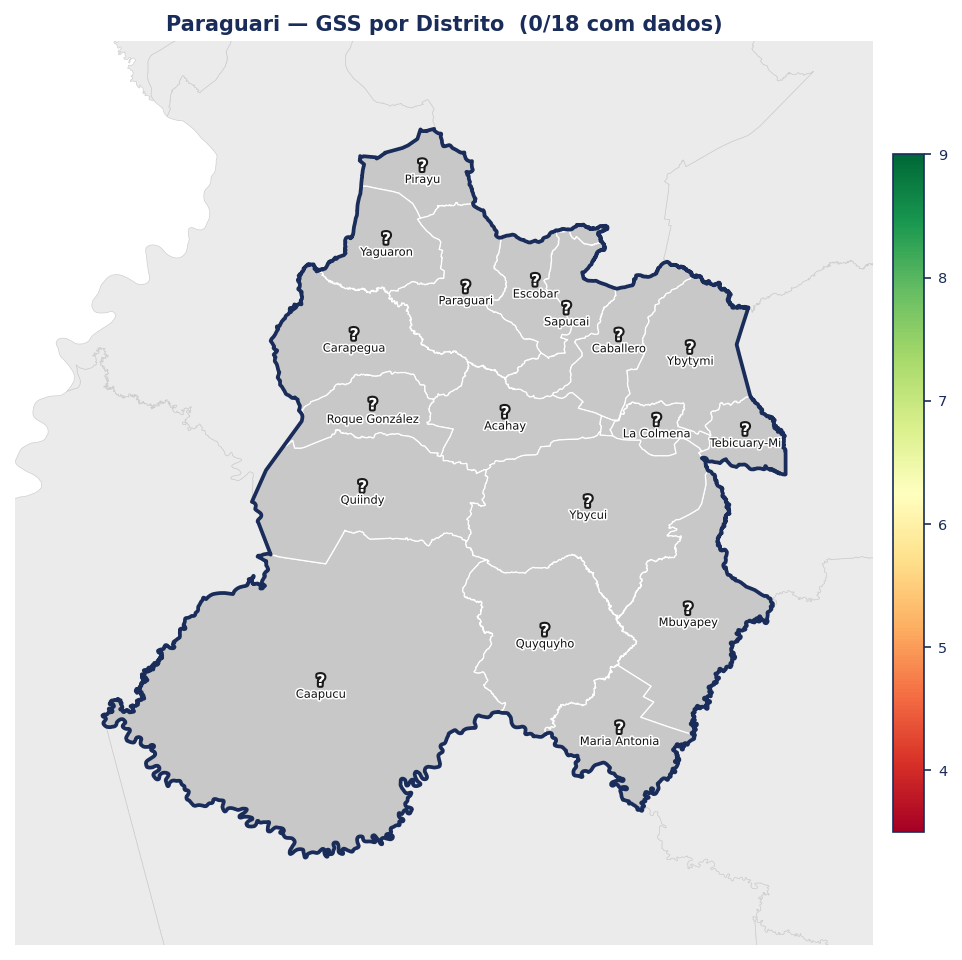
\includegraphics[width=\textwidth, height=0.55\textheight, keepaspectratio]{mapas/mapas_tematicos_dept_09_gss.png}
\caption{GSS (Global Safety Score) por distrito de Paraguari. Verde = alta viabilidade · Vermelho = baixa viabilidade.}
\label{fig:gss-09}
\end{figure}

\vspace{0.5em}

\begin{figure}[htbp]
\centering
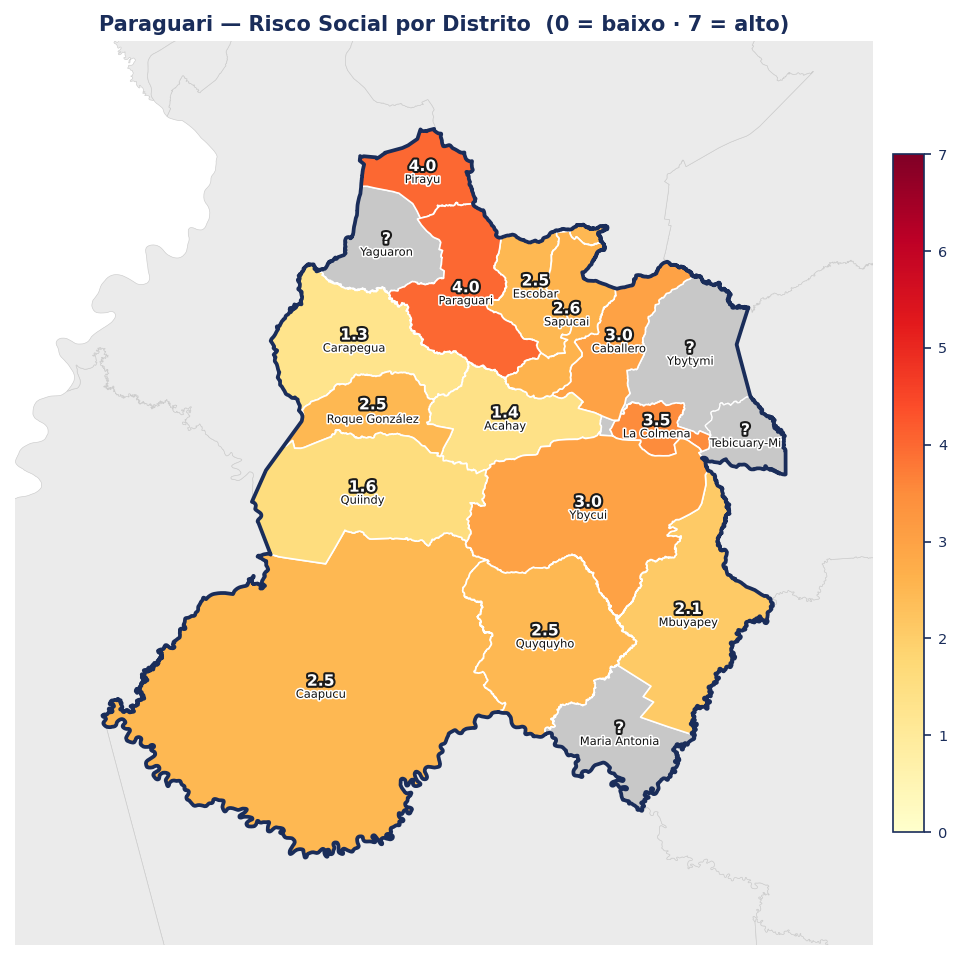
\includegraphics[width=\textwidth, height=0.55\textheight, keepaspectratio]{mapas/mapas_tematicos_dept_09_risco.png}
\caption{Risco social por distrito de Paraguari. Amarelo = baixo risco · Vermelho = alto risco.}
\label{fig:risco-09}
\end{figure}

\clearpage

\begin{figure}[htbp]
\centering
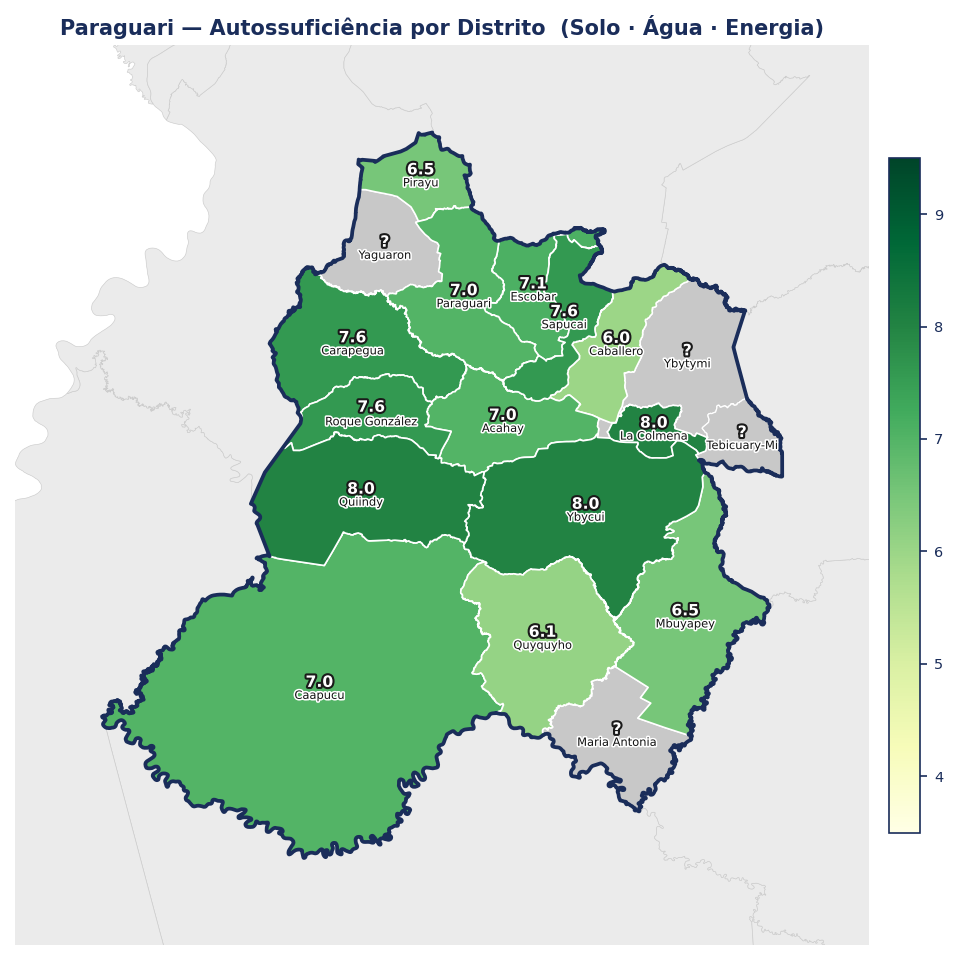
\includegraphics[width=\textwidth, height=0.55\textheight, keepaspectratio]{mapas/mapas_tematicos_dept_09_autosuf.png}
\caption{Autossuficiência por distrito de Paraguari: solo, recursos hídricos e potencial energético. Branco = baixo · Verde escuro = alto.}
\label{fig:autosuf-09}
\end{figure}

\clearpage

\section{Paraguarí}

serrania protegida, base militar estratégica e boa conectividade com
Assuncao via PY01.

\subsection{Ficha climática de Paraguari (capital
departamental)}

\textbf{Irradiância solar global --- (kWh/\allowbreak m²/\allowbreak dia):}


\begin{center}
\resizebox{\linewidth}{!}{%
{\renewcommand{\arraystretch}{1.2}%
\begin{tabular}{@{}c|c|c|c|c|c|c|c|c|c|c|c@{}}
\toprule
Jan & Fev & Mar & Abr & Mai & Jun & Jul & Ago & Set & Out & Nov & Dez \\
\midrule
6.76 & 6.20 & 5.42 & 4.44 & 3.36 & 2.83 & 3.21 & 3.93 & 4.61 & 5.49 &
6.42 & 6.78 \\
\bottomrule
\end{tabular}}%
}
\end{center}


Média anual: 4.95 kWh/\allowbreak m²/\allowbreak dia. Inclinação recomendada: 26° Norte (anual);
36° inverno; 16° verão.

\textbf{Precipitação --- (mm/\allowbreak mês):}


\begin{center}
\resizebox{\linewidth}{!}{%
{\renewcommand{\arraystretch}{1.2}%
\begin{tabular}{@{}c|c|c|c|c|c|c|c|c|c|c|c@{}}
\toprule
Jan & Fev & Mar & Abr & Mai & Jun & Jul & Ago & Set & Out & Nov & Dez \\
\midrule
127 & 140 & 133 & 148 & 152 & 78 & 66 & 41 & 77 & 171 & 193 & 175 \\
\bottomrule
\end{tabular}}%
}
\end{center}


Média anual: \textasciitilde1.500 mm/\allowbreak ano. Estação chuvosa Out-Nov; seca
Jun-Ago.
\clearpage
\subsection*{Dados Departamentais}

\subsection*{Segurança Pública}

\begin{tabularx}{\linewidth}{lX}
\toprule
Indicador & Valor \\
\midrule
Taxa de homicídios (por 100k hab) & ~3,0 (estimativa, abaixo da média nacional) \\
Crimes registrados (total/ano) & --- dados não desagregados publicamente \\
Número de comisarías & ~15 (estimativa departamental) \\
Índice segurança relativo & alto \\
\bottomrule
\end{tabularx}

Paraguarí é historicamente reconhecido como um dos departamentos mais seguros do Paraguai. Pesquisas do CONACYT e dados do INE apontam que Paraguarí, junto com Cordillera e Central, mantêm uma das mais baixas taxas de homicídio do país, com \textbf{média histórica de aproximadamente 3 mortes por 100 mil habitantes}.

O Ministerio Público registra que o departamento responde por apenas \textbf{1\% das causas de homicídio doloso} nacional (2019--2024) --- uma das menores proporções do país para um departamento de tamanho médio. Paraguarí não possui fronteira internacional e está localizado no centro-sul do Paraguai, distante das rotas principais de narcotráfico.

A economia é baseada em agricultura familiar, pecuária e, em alguns municípios, turismo. Paraguarí (cidade capital) e Carapeguá são os maiores centros urbanos. A criminalidade é de baixa intensidade, predominantemente patrimonial.

\subsection*{IDH e Desenvolvimento Humano}

\begin{tabularx}{\linewidth}{lX}
\toprule
Indicador & Valor \\
\midrule
IDH & 0,706 \\
Classificação IDH & alto \\
Ranking nacional (1=melhor) & 9/18 \\
Esperança de vida & 72,6 anos \\
Anos de escolaridade média & 8,1 anos \\
RNB per capita (USD PPA) & 8.500 \\
\bottomrule
\end{tabularx}

> Nota: IDH estimado com base no relatório PNUD 2020 e dados subnacionais regionais. Paraguarí está próximo a Cordillera em perfil socioeconômico, com importante corredor produtivo (algodão, mandioca, pecuária) e acesso à capital pela Rota 1.

\begin{tabularx}{\linewidth}{lX}
\toprule
Indicador & Valor \\
\midrule
Taxa de pobreza total (\%) & 30,5\% \\
Taxa de pobreza extrema (\%) & 7,1\% \\
Índice de Gini & 0,453 \\
\bottomrule
\end{tabularx}

> Fonte: INE --- EPHC 2023 (dado de 30,5\% confirmado para Paraguarí). Pobreza multidimensional (IPM) de 26,77\% em 2023, um dos departamentos com índice multidimensional mais alto entre os da Região Oriental central.

\begin{tabularx}{\linewidth}{lX}
\toprule
Indicador & Valor \\
\midrule
Acesso a água potável (\%) & 77,6\% \\
Acesso a saneamento (\%) & 75,8\% \\
\bottomrule
\end{tabularx}

> Estimativa baseada em dados do Censo 2022. Paraguarí tem boa conectividade pela Rota 1 (Asunción--Encarnación), o que favorece o acesso a serviços em cidades próximas.

Paraguarí tem IDH alto (0,706) e é cortado pela principal rodovia do Paraguai (Rota 1), que liga Asunción ao sul do país. A capital departamental Paraguarí é cidade pequena mas bem conectada. O departamento tem potencial turístico (Parque Nacional Ybycuí, Chololo) e agropecuário. Para brasileiros, pode ser interessante como moradia com fácil acesso a Asunción (1--1,5h), combinando custo baixo com qualidade de vida razoável. A pobreza de 30,5\% e o IPM de 26,77\% indicam desigualdades internas. O acesso a água (77,6\%) e saneamento (75,8\%) são medianos --- melhores na capital departamental, piores nas zonas rurais. Oportunidades em agricultura, pecuária e turismo.

\subsection*{Sistema Prisional}

{\small
{\small
\begin{tabularx}{\linewidth}{lXXXX}
\toprule
Nome & Município & Capacidade & População & Superlotação \\
\midrule
Penitenciaría Regional de Paraguarí & Paraguarí & 150 & ~280 & ~187\% \\
\bottomrule
\end{tabularx}
}
}

\begin{tabularx}{\linewidth}{lX}
\toprule
Indicador & Valor \\
\midrule
Total de estabelecimentos & 1 \\
Capacidade total (vagas) & ~150 \\
População carcerária total & ~280 \\
Taxa de superlotação & ~187\% \\
\% presos provisórios & ~66\% \\
\bottomrule
\end{tabularx}

O departamento de Paraguarí conta com uma única penitenciaría regional, em sua capital homônima. O estabelecimento atende detentos dos 17 municípios do departamento, incluindo Carapeguá, Ybycuí, La Colmena e Acahay.

Paraguarí tem localização privilegiada: faz fronteira com o departamento Central e está a cerca de 60--80 km de Asunción. Isso facilita o acesso a serviços da capital, mas também cria pressão adicional sobre o sistema de justiça local, que recebe casos transbordados da região metropolitana.

O perfil criminal é predominantemente de crimes contra a propriedade, violência doméstica e pequeno tráfico de drogas. Não há presença significativa de crime organizado de grande escala.

\textbf{Para imigrantes:} Paraguarí é um departamento com boa qualidade de vida e proximidade com Asunción. Municípios como Carapeguá e Ybycuí têm crescimento urbano moderado e oferecem oportunidades para residência e negócios de menor escala. A presença do presídio em Paraguarí tem impacto mínimo na segurança geral do departamento.

\subsection*{Recursos Hídricos Subterrâneos}

\begin{tabularx}{\linewidth}{lXXX}
\toprule
Aquífero & Cobertura no Dept. & Profundidade Média & Vazão Típica \\
\midrule
Patiño (freático, porção norte) & ~25\% & 30--100 m & 5--15 m$^3$/h \\
Guarani / Misiones (confinado) & ~60\% & 100--400 m & 20--70 m$^3$/h \\
Cristalino (fraturado, Serra de Paraguarí) & ~15\% & 30--80 m & 2--8 m$^3$/h \\
\bottomrule
\end{tabularx}

\begin{tabularx}{\linewidth}{lX}
\toprule
Parâmetro & Valor \\
\midrule
Profundidade média --- Patiño (m) & 30--100 \\
Profundidade média --- Guarani (m) & 100--400 \\
Profundidade máxima recomendada (m) & 450 \\
Vazão típica (m$^3$/h) & 5--50 \\
Custo estimado perfuração (USD) & 2.500 -- 10.000 \\
Qualidade da água --- Patiño & boa a moderada \\
Qualidade da água --- Guarani & boa a excelente \\
pH médio & 6,5--7,5 \\
Outorga necessária & sim \\
Órgão regulador & MADES --- DGPCRH \\
\bottomrule
\end{tabularx}

Paraguarí é o departamento onde o Aquífero Patiño tem sua extensão sul, antes de passar a ser dominado pelo sistema Guarani/Misiones. A Serra de Paraguarí (embasamento cristalino) oferece captação em fraturas com boa qualidade. O Aquífero Guarani é acessível na porção centro-sul do departamento. A qualidade geral é boa. A cidade de Paraguarí (capital) e Carapeguá têm redes públicas do SENASA. Para propriedades rurais na Serra de Ybycuí e arredores, o cristalino com captação rasa é opção econômica. Uso principal: doméstico e pecuária.

Paraguarí combina paisagem serrana com proximidade de Asunción (~70 km). Para sítios e chácaras perto da capital, o Aquífero Patiño (30--80 m) oferece captação econômica (USD 2.500--6.000). No sul do departamento, o Guarani (100--250 m) garante vazão robusta para propriedades maiores. Ybycuí, com seu Parque Nacional, é área de crescente interesse para residência. A Serra de Ybycuí tem aquíferos cristalinos com boa qualidade. Sempre exigir licença do MADES antes de perfurar.

\subsection*{Aptidão do Solo}

\begin{tabularx}{\linewidth}{lXX}
\toprule
Tipo de Solo & \% do Território & Características \\
\midrule
Ultissolos (Argissolos) & 45\% & Solos podzólicos com horizonte B textural, textura areno-argilosa, fertilidade baixa a média \\
Entissolos arenosos & 30\% & Solos arenosos derivados de arenito, baixa retenção hídrica, muito suscetíveis à erosão \\
Inceptissolos & 15\% & Solos em formação, encostas e serras (Cordilheira de los Altos); moderada fertilidade \\
Oxissolos (fragmentados) & 10\% & Pequenas manchas de solos basálticos no sul do departamento \\
\bottomrule
\end{tabularx}

\begin{tabularx}{\linewidth}{lXX}
\toprule
Classe & \% Território & Uso Recomendado \\
\midrule
Lavoura intensiva & 5\% & Apenas nas pequenas manchas de Oxissolos \\
Lavoura extensiva & 25\% & Mandioca, milho, amendoim, cana-de-açúcar \\
Pastagem natural/melhorada & 35\% & Pecuária extensiva \\
Floresta / reserva & 25\% & Serras, matas ciliares, área de recarga hídrica \\
Sem aptidão agrícola & 10\% & Afloramentos rochosos, áreas urbanas, solos severamente erodidos \\
\bottomrule
\end{tabularx}

\begin{tabularx}{\linewidth}{lX}
\toprule
Parâmetro & Valor \\
\midrule
pH médio & 4,8 -- 5,5 \\
Fertilidade natural & baixa \\
Teor de matéria orgânica & baixo \\
Necessidade de calcário & sim \\
\bottomrule
\end{tabularx}

Paraguarí apresenta baixo interesse para imigrantes brasileiros com perfil agrícola empresarial. Os solos figuram entre os mais degradados e limitados do Paraguai. O terreno acidentado, a acidez elevada e a histórica exploração predatória dificultam recuperação produtiva em curto prazo. A proximidade com Asunción (~65 km) é um aspecto positivo para comércio e prestação de serviços. Para quem busca sítios de lazer ou agroturismo nas serras, pode haver nichos interessantes. Para agricultura intensiva ou pecuária tecnificada, há opções muito melhores no país.

\subsection*{Terra Rural}

\begin{tabularx}{\linewidth}{lXXX}
\toprule
Tipo & Preço (USD/ha) & Faixa & Tendência \\
\midrule
Agrícola alta produtividade & 4.800 & 3.200 -- 7.000 & $\uparrow$ \\
Pastagem & 2.400 & 1.600 -- 3.500 & $\uparrow$ \\
Mata / reserva & 1.000 & 600 -- 1.800 & $\rightarrow$ \\
\bottomrule
\end{tabularx}

> Referência de listagem observada: USD 2.400/ha para terras mistas em Paraguarí.

\begin{tabularx}{\linewidth}{lX}
\toprule
Parâmetro & Valor \\
\midrule
Valorização anual média (\%) & 6--8\% \\
Lote mínimo rural (ha) & 10 \\
Imposto territorial rural (\%) & 1\% sobre valor fiscal \\
Liquidez do mercado & média \\
\bottomrule
\end{tabularx}

\begin{tabularx}{\linewidth}{lXXX}
\toprule
Indicador & Paraguarí (PY) & São Paulo interior (BR) & Paraná (BR) \\
\midrule
Terra agrícola (USD/ha) & 3.200--7.000 & 20.000--45.000 & 15.000--30.000 \\
Chácara de lazer (USD/ha) & 4.000--9.000 & 30.000--80.000 & 15.000--40.000 \\
Custo relativo & ~20\% do SP & referência SP & referência PR \\
\bottomrule
\end{tabularx}

Paraguarí é atrativo para quem deseja chácara de lazer perto de Asunción a custos muito menores do que os equivalentes nas periferias das capitais estaduais brasileiras.

\subsection*{Mercado Imobiliário}

\textbf{Capital:} Paraguarí

\begin{tabularx}{\linewidth}{lXX}
\toprule
Tipo & Preço (USD/m$^2$) & Aluguel (USD/mês) \\
\midrule
Apartamento 2 quartos & 550 -- 850 & 200 -- 380 \\
Casa 3 quartos & 480 -- 750 & 180 -- 340 \\
\bottomrule
\end{tabularx}

\begin{tabularx}{\linewidth}{lX}
\toprule
Parâmetro & Valor \\
\midrule
Valorização anual (\%) & 5--7\% \\
Disponibilidade de financiamento & boa (proximidade com Asunción facilita acesso a bancos nacionais) \\
Bairros mais valorizados & Centro, Barrio San José, proximidades da estação ferroviária histórica \\
\bottomrule
\end{tabularx}

\textbf{Vale a pena comprar ou alugar?}
Paraguarí é uma opção interessante para quem trabalha em Asunción mas prefere morar no interior. A cidade fica a 70 km da capital pela Ruta 1 (45--60 min). Custo de vida notavelmente mais baixo que Asunción com qualidade de vida superior em termos de espaço e ambiente. A compra de casa é geralmente vantajosa.

\textbf{Áreas recomendadas:}
A cidade de Paraguarí e Carapeguá (conhecida pelo artesanato de ñandutí) são as melhores opções do departamento, com infraestrutura razoável e bom acesso à Ruta 1 em direção a Asunción. Paraguarí cidade oferece estação ferroviária e acesso rodoviário direto à capital.

\textbf{Armadilhas comuns:}
Imóveis antigos no departamento frequentemente não possuem registro de benfeitorias realizadas ao longo dos anos, o que pode gerar discrepâncias entre a metragem construída na escritura e a realidade física. Solicite laudo de medição e vistoria técnica antes de fechar o negócio.

\subsection*{Cobertura Celular}

{\small
{\small
\begin{tabularx}{\linewidth}{lXXXXX}
\toprule
Operadora & 2G & 3G & 4G & 5G & Cobertura Pop. \\
\midrule
Tigo & 92\% & 85\% & 75\% & --- & 88\% \\
Personal/Claro & 88\% & 80\% & 70\% & --- & 84\% \\
VOX & 60\% & 45\% & 28\% & --- & 52\% \\
\bottomrule
\end{tabularx}
}
}

> \textbf{Nota:} Paraguarí é um departamento próximo a Asunción (capital a ~60 km) com boa cobertura de telecomunicações. A Ruta 1 e Ruta 2 cruzam o departamento, garantindo cobertura linear sólida. Municípios turísticos como Paraguarí, Caapucú e Sapucái têm boa cobertura.

\begin{tabularx}{\linewidth}{lX}
\toprule
Parâmetro & Valor \\
\midrule
Melhor operadora rural & Tigo \\
Velocidade 4G média (Mbps) & 22--42 \\
Áreas sem cobertura & Interior serrano, zonas de mata no sul \\
Sinal em propriedade rural & bom a moderado \\
\bottomrule
\end{tabularx}

\begin{tabularx}{\linewidth}{lXXX}
\toprule
Plano & Operadora & USD/mês & Dados \\
\midrule
Pré-pago básico (7 dias) & Tigo & ~2,50 & 3 GB \\
Pré-pago intermediário (30 dias) & Personal & ~5,00 & 8 GB \\
Pós-pago entrada & Tigo & ~12,00 & 15 GB + chamadas \\
Pós-pago intermediário & Personal/Claro & ~18,00 & 30 GB + chamadas \\
\bottomrule
\end{tabularx}

\subsection*{Internet}

\begin{tabularx}{\linewidth}{lX}
\toprule
Indicador & Valor \\
\midrule
\% população com internet & ~68\% \\
\% com banda larga fixa & ~25\% dos domicílios \\
Velocidade média download (Mbps) & 30--70 (urbano) / 6--18 (rural) \\
Velocidade média upload (Mbps) & 10--25 (urbano) \\
\bottomrule
\end{tabularx}

> Paraguarí se beneficia da proximidade com a área metropolitana de Asunción, com melhor conectividade que departamentos mais distantes da capital.

\begin{tabularx}{\linewidth}{lXX}
\toprule
Tecnologia & Disponibilidade & Velocidade Típica \\
\midrule
Fibra ótica (FTTH) & Paraguarí cidade, Carapeguá, Quiindy & 50--300 Mbps \\
Cabo HFC & Paraguarí cidade & 30--150 Mbps \\
Rádio/Wireless & Amplo no departamento & 5--50 Mbps \\
ADSL (Copaco) & Interior com rede legada & 2--10 Mbps \\
Satélite (Starlink) & Todo o departamento & 50--200 Mbps \\
\bottomrule
\end{tabularx}

\begin{tabularx}{\linewidth}{lXXX}
\toprule
Provedor & Tecnologia & Área de cobertura & Preço ref. (USD/mês) \\
\midrule
Tigo & Fibra/HFC/Rádio & Paraguarí + municípios principais & 18--55 \\
Claro/Personal & Fibra/Rádio & Paraguarí cidade + Carapeguá & 15--50 \\
Copaco & ADSL/Fibra & Interior & 10--28 \\
Starlink & Satélite LEO & Todo o departamento & ~44 + equip. ~370 \\
\bottomrule
\end{tabularx}

A cobertura rural de Paraguarí é \textbf{moderada}, boa ao longo das rotas principais e mais limitada no interior:

\clearpage
\newpage
\secaoDiagnostico{Acahay}{\mapaDistrito{0902}}{Acahay (Paraguari) apresenta perfil operacional consolidado para
comparacao territorial, com leitura conjunta de infraestrutura, risco
hidroclimatico e capacidade de continuidade de servicos essenciais.

\subsubsection{Pre-condicoes Minimas de
Decisao}

\begin{itemize}
\tightlist
\item
  Atualizar indicadores criticos em ciclo trimestral.
\item
  Confirmar trafegabilidade e contingencia hidrica/\allowbreak energetica local.
\item
  Validar checklist de resiliencia domiciliar/\allowbreak logistica antes de decisao
  final.
\end{itemize}

\subsubsection{Recomendação
Técnica}

Uso recomendado como candidato em analise multicriterio, condicionado ao
cumprimento das pre-condicoes acima. Referência atual de score: GSS 8.1;
risco predominante: baixo.

}
\begin{table}[ht!]
\small \begin{tabular}{p{3.0cm}p{0.8cm}p{6.0cm}} \toprule
\textbf{Critério} & \textbf{Nota} & \textbf{Justificativa} \\ \midrule
A - Ameaças Estratégicas & 8.6 & - \\
B - Risco Social & 8.6 & - \\
C - Riscos Naturais & 7.2 & - \\
D - Autossuficiência & 7.0 & - \\
E - Institucional & 8.5 & - \\
\midrule
 \textbf{GSS FINAL} & \textbf{8.1} & \textbf{Seguro (bom potencial com preparacao).} \\ \bottomrule
 \end{tabular}
\end{table}
\subsubsection{Vulnerabilidades e
Mitigação}\label{vuln-Acahay-vulnerabilidades-e-mitigauxe7uxe3o}

\begin{itemize}
\tightlist
\item
  Exposicao hidrometeorologica controlada (\textless45/\allowbreak 100).
\item
  Conectividade viaria favoravel (\textgreater=70/\allowbreak 100).
\item
  Estoque de contingencia para 14 dias (agua/\allowbreak alimentos/\allowbreak combustivel),
  priorizado quando risco hidro=35/\allowbreak 100.
\item
  Duplicar rotas/\allowbreak logistica quando conectividade viaria=89/\allowbreak 100 for
  \textless70; manter rota secundaria mapeada e testada trimestralmente.
\item
  Plano de energia resiliente com autonomia minima de 72h
  (geracao/\allowbreak backup), revisao semestral.
\end{itemize}

\subsubsection{Dossiê de Campo}\label{dossie-Acahay-dossiuxea-de-campo}
\begin{description}[style=nextline,leftmargin=0.5cm,font=\bfseries]
\item[Coordenadas]  25°55'S 57°07'W (geocodificado via Nominatim).
\end{description}
\textbf{Fonte climática:} NASA POWER Climatology API (período 2001-2020)

\textbf{Fonte luminosa:} estimativa world atlas

\paragraph{Irradiação Solar
(kWh/\allowbreak m²/\allowbreak dia)}


\begin{center}
\resizebox{\linewidth}{!}{%
{\renewcommand{\arraystretch}{1.2}%
\begin{tabular}{@{}c|c|c|c|c|c|c|c|c|c|c|c|c@{}}
\toprule
Jan & Fev & Mar & Abr & Mai & Jun & Jul & Ago & Set & Out & Nov & Dez & Média \\
\midrule
6.76 & 6.20 & 5.42 & 4.44 & 3.36 & 2.83 & 3.21 & 3.93 & 4.61 & 5.49 &
6.42 & 6.78 & \textbf{4.95} \\
\bottomrule
\end{tabular}}%
}
\end{center}


\textbf{Inclinação solar recomendada:} 26° N (anual) · 36° N (inverno
jun-ago) · 16° N (verão nov-jan)

\paragraph{Precipitação (mm/\allowbreak mês)}


\begin{center}
\resizebox{\linewidth}{!}{%
{\renewcommand{\arraystretch}{1.2}%
\begin{tabular}{@{}c|c|c|c|c|c|c|c|c|c|c|c|c@{}}
\toprule
Jan & Fev & Mar & Abr & Mai & Jun & Jul & Ago & Set & Out & Nov & Dez & Total/\allowbreak ano \\
\midrule
132 & 126 & 133 & 157 & 157 & 86 & 73 & 55 & 87 & 181 & 187 & 168 &
\textbf{1544 mm} \\
\bottomrule
\end{tabular}}%
}
\end{center}


\paragraph{Poluição Luminosa}

\begin{longtable}[]{@{}ll@{}}
\toprule\noalign{}
Parâmetro & Valor \\
\midrule\noalign{}
\endhead
\bottomrule\noalign{}
\endlastfoot
Escala Bortle & 3 --- Céu rural \\
Radiância artificial & 1.5 nW/\allowbreak cm²/\allowbreak sr \\
\end{longtable}
\paragraph{Solo (SoilGrids 2.0, média ponderada 0--30
cm)}

\begin{longtable}[]{@{}ll@{}}
\toprule\noalign{}
Parâmetro & Valor \\
\midrule\noalign{}
\endhead
\bottomrule\noalign{}
\endlastfoot
pH (H$_2$O) & 5.5 \\
Carbono orgânico (SOC) & 18.64 g/\allowbreak kg \\
Argila & 26.22 \% \\
Areia & 53.1 \% \\
Silte (calc.) & 20.7 \% \\
Densidade aparente & 1.29 g/\allowbreak cm³ \\
\textbf{Aptidão agrícola} & \textbf{Alta} \\
\end{longtable}

\subsubsection{Indicadores Sociais}

\textbf{Fontes:} PNUD 2020, INE\footnote{\fineINE} Censo 2022, INE\footnote{\fineINE} EPHC 2023, Ministerio
Público 2024\\
\textbf{Nota:} Valores marcados como \emph{(dept.)} referem-se ao
departamento de Paraguarí; valores \emph{(dist.)} são específicos deste
distrito. Dados marcados \emph{(est.)} são estimativas.

\begin{longtable}[]{@{}
  >{\raggedright\arraybackslash}p{(\linewidth - 4\tabcolsep) * \real{0.4231}}
  >{\raggedright\arraybackslash}p{(\linewidth - 4\tabcolsep) * \real{0.2692}}
  >{\raggedright\arraybackslash}p{(\linewidth - 4\tabcolsep) * \real{0.3077}}@{}}
\toprule\noalign{}
\begin{minipage}[b]{\linewidth}\raggedright
Indicador
\end{minipage} & \begin{minipage}[b]{\linewidth}\raggedright
Valor
\end{minipage} & \begin{minipage}[b]{\linewidth}\raggedright
Âmbito
\end{minipage} \\
\midrule\noalign{}
\endhead
\bottomrule\noalign{}
\endlastfoot
IDH (2020) & 0,706 & dept. \\
Ranking IDH nacional & 9/\allowbreak 18 & dept. \\
Esperança de vida & 72,6 anos & dept. \\
Escolaridade média & 8.1 anos & dist. \\
RNB per capita (USD PPA) & 8.500 & dept. \\
Pobreza monetária (\%) & 30,5\% & dept. \\
Pobreza extrema (\%) & 7,1\% & dept. \\
Índice de Gini & 0,453 & dept. \\
Acesso a água potável (\%) & 77,6\% & dept. \\
Acesso a saneamento (\%) & 75,8\% & dept. \\
Taxa de homicídios (est., /\allowbreak 100k hab) & \textasciitilde3,0 (estimativa,
abaixo da média nacional) & dept. \\
Índice de segurança & alto & dept. \\
População (Censo 2022) & 12.646 hab. & dist. \\
Idade mediana & 33.0 anos & dist. \\
Taxa de fecundidade & N/\allowbreak D & dist. \\
\end{longtable}
\subsubsection{Combustível}

\textbf{Referência:} PETROPAR /\allowbreak  postos locais (2024) \textbf{Tipo de
localidade:} Interior

\begin{longtable}[]{@{}lll@{}}
\toprule\noalign{}
Combustível & USD/\allowbreak litro & Gs/\allowbreak litro (aprox.) \\
\midrule\noalign{}
\endhead
\bottomrule\noalign{}
\endlastfoot
Gasolina 93 oct & 0.97 & 7,178 \\
Gasolina 97 oct (premium) & 1.07 & 7,918 \\
Diesel & 0.90 & 6,660 \\
\end{longtable}

\begin{quote}
Preços podem variar ±5\% conforme posto e sazonalidade. Chaco e interior
remoto apresentam maior variação.
\end{quote}

\subsubsection{Cobertura Celular}

\textbf{Fonte:} CONATEL PY /\allowbreak  operadoras (2024)

\begin{longtable}[]{@{}ll@{}}
\toprule\noalign{}
Parâmetro & Valor \\
\midrule\noalign{}
\endhead
\bottomrule\noalign{}
\endlastfoot
Cobertura 4G população (dept.) & 88\% \\
Cobertura 4G área rural & 72\% \\
Melhor operadora & Tigo \\
Qualidade rural & boa \\
\end{longtable}

\begin{quote}
Para áreas rurais fora do núcleo urbano, recomenda-se chip Tigo como
principal e Personal como backup.
\end{quote}

\subsubsection{Internet}

\textbf{Fonte:} CONATEL /\allowbreak  Speedtest Ookla (2024)

\begin{longtable}[]{@{}ll@{}}
\toprule\noalign{}
Parâmetro & Valor \\
\midrule\noalign{}
\endhead
\bottomrule\noalign{}
\endlastfoot
Velocidade média download & 50 Mbps \\
Domicílios com internet (dept.) & 58\% \\
Tecnologia predominante & rádio \\
Opção rural & Starlink disponível (\textasciitilde USD 44/\allowbreak mês) \\
\end{longtable}

\subsubsection{Mercado Imobiliário e Terra
Rural}

\textbf{Fonte:} INDERT /\allowbreak  Clasificados.com.py (2024)

\begin{longtable}[]{@{}ll@{}}
\toprule\noalign{}
Tipo & Referência \\
\midrule\noalign{}
\endhead
\bottomrule\noalign{}
\endlastfoot
Terra agrícola alta prod. (USD/\allowbreak ha) & 4,500 \\
Imóvel urbano (USD/\allowbreak m²) & 700 \\
Aluguel 2 quartos (USD/\allowbreak mês) & 280 \\
\end{longtable}

\begin{quote}
Valores de referência departamental. Localidades menores podem ter
preços 20--40\% abaixo da capital departamental. \#\#\# Saúde
\end{quote}

\textbf{Fonte:} MSPBS /\allowbreak  IPS Paraguay (2024-2026), consolidação
departamental e proxy local

\begin{longtable}[]{@{}ll@{}}
\toprule\noalign{}
Serviço & Disponibilidade \\
\midrule\noalign{}
\endhead
\bottomrule\noalign{}
\endlastfoot
USF /\allowbreak  Posto de Saúde & sim \\
Hospital Regional & não \\
IPS (seguro social) & não \\
Farmácia & sim \\
Distância ao hospital de referência & \textasciitilde41 km
(Paraguari) \\
\end{longtable}

\textbf{Principais estabelecimentos:} USF local; referencia hospitalar
em Paraguari

\textbf{Observação para imigrantes:} Atendimento primario local ou em
raio curto; casos de maior complexidade seguem para Paraguari. Cobertura
privada continua recomendada para especialidades e urgências de maior
complexidade.
\newpage
\secaoDiagnostico{Caapucu}{\mapaDistrito{0903}}{Caapucú oferece um dos maiores potenciais de privacidade demográfica e
isolamento tático da Região Oriental do Paraguai. Sua força reside na
vastidão territorial combinada com uma densidade populacional baixíssima
e segurança social superior. Oferece solo apto para pecuária e
abundância de recursos hídricos (Rio Tebicuary), sendo o local ideal
para quem busca um refúgio rural autêntico e discreto, aceitando a
necessidade de autonomia logística e de saúde.

\subsubsection{Recomendação
Técnica}

Altamente indicado para estabelecimentos de autossuficiência de
médio/\allowbreak grande porte ou estâncias pecuárias que busquem isolamento
demográfico massivo. Requer autonomia em logística básica e saúde. O GSS
de 6.5 reflete a segurança do isolamento em contraste com a limitação
institucional local. Referência atual de score: GSS 6.5.

}
\begin{table}[ht!]
\small \begin{tabular}{p{3.0cm}p{0.8cm}p{6.0cm}} \toprule
\textbf{Critério} & \textbf{Nota} & \textbf{Justificativa} \\ \midrule
A - Ameaças Estratégicas & 6.0 & Localização discreta e fora de eixos de conflito primário; boa invisibilidade tática \\
B - Risco Social & 7.5 & Baixíssima densidade demográfica em território vasto; isolamento social superior \\
C - Riscos Naturais & 7.0 & Geologia muito estável e riscos naturais climáticos típicos manejáveis \\
D - Autossuficiência & 7.0 & Excelentes recursos naturais - gado e água - mas limitado pela escala logística local \\
E - Institucional & 5.0 & Município seguro, mas com infraestrutura institucional e de saúde básica limitada \\
\midrule
 \textbf{GSS FINAL} & \textbf{6.5} & \textbf{Moderadamente Seguro (Ideal para quem busca o máximo de isolamento demográfico em território produtivo e seguro).} \\ \bottomrule
 \end{tabular}
\end{table}
\subsubsection{Vulnerabilidades e
Mitigação}\label{vuln-Caapucu-vulnerabilidades-e-mitigauxe7uxe3o}

\begin{itemize}
\tightlist
\item
  \textbf{Isolamento de Saúde:} Distância significativa de centros
  hospitalares cirúrgicos (Mitigação: manutenção de estoque médico
  básico e kit trauma local).
\item
  \textbf{Logística Interna:} Acesso terrestre precário em chuvas
  intensas em estâncias remotas (Mitigação: estoque de suprimentos para
  60 dias e posse de veículo 4x4 robusto).
\item
  \textbf{Risco de Inundação:} Evitar áreas ribeirinhas do Rio Tebicuary
  (Mitigação: construção em cotas \textgreater120m).
\end{itemize}

\subsubsection{Dossiê de Campo}\label{dossie-Caapucu-dossiuxea-de-campo}
\begin{description}[style=nextline,leftmargin=0.5cm,font=\bfseries]
\item[Coordenadas]  26°13'S 57°12'W.
\item[Topografia]  Relevo plano a suavemente ondulado, localizado no sul do departamento, margeado pelo Rio Tebicuary. Altitude \textasciitilde 110m. Área vasta de \textasciitilde 2.486 km². Geologicamente muito estável, risco sísmico desprezível.
\item[Alvos Estratégicos]  Áreas de pecuária extensiva; Ponto de transição logística na Ruta PY01 (Eixo Assunção-Sul). Ausência de alvos militares ou industriais de grande porte, oferecendo excelente invisibilidade estratégica em território vasto.
\item[Fallout]  Ventos predominantes do Norte (NE) e Leste. Baixo risco de fallout direto.
\item[População]  6.838 habitantes (Censo 2022 Final). Perfil demográfico rural disperso em grandes estâncias e pequenas companhias rurais.
\item[Densidade]  \textasciitilde 2,75 hab/\allowbreak km² (Densidade extremamente baixa, uma das menores do país na Região Oriental, oferecendo isolamento tático e privacidade estratégica superior).
\item[Vias de Acesso]  Localização privilegiada sobre a Ruta PY01 (Asfaltada). Conectividade de elite para o Sul (Misiones) e a capital. Malha interna de estradas de terra que exigem veículos robustos em períodos chuvosos (média 1.500 mm/\allowbreak ano).
\item[Serviços]  Unidade de Saúde da Família (USF) local. Dependência de Carapeguá ou San Ignacio (Misiones) para saúde de alta complexidade e logística comercial diversificada.
\item[Custo de Vida]  Muito baixo; economia estritamente vinculada à pecuária de corte.
\item[Preço da Terra]  US\$ 2.000-3.500/\allowbreak ha (áreas de campo natural/\allowbreak pecuária); US\$ 5.000/\allowbreak ha (áreas próximas à rodovia).
\item[Hidrologia]  Risco Moderado de Inundação. Presença do Rio Tebicuary e seus arroios tributários. Áreas ribeirinhas baixas vulneráveis a transbordamentos cíclicos em anos de El Niño intenso. Drenagem natural eficiente no relevo ondulado.
\item[Clima]  Subtropical Úmido. Verões quentes e invernos secos.
\item[Energia]  Rede nacional (Itaipu/\allowbreak Yacyretá); instável em áreas rurais remotas.
\item[Água]  Abundante via poços artesianos e lençol freático produtivo; proximidade com o Rio Tebicuary.
\item[Qualidade do Solo]  Solo predominantemente arenoso e hidromórfico nas baixadas; fértil para pastagens e agricultura familiar de subsistência.
\item[Recursos Locais]  Grande produção de gado de corte e leite. Elevadíssimo potencial para autossuficiência hídrica e proteica per capita devido à baixíssima carga demográfica.
\item[Segurança]  Zona rural extremamente pacífica e estável. Baixíssima criminalidade urbana. Coesão social forte baseada em comunidades tradicionais laboriosas. Baixa visibilidade para conflitos de massa.
\item[Leis Local: Município histórico e consolidado. Livre de Restrição de Fronteira]  Fora da faixa de 50km da fronteira internacional.
\end{description}
\textbf{Fonte climática:} NASA POWER Climatology API (período 2001-2020)

\textbf{Fonte luminosa:} estimativa world atlas

\paragraph{Irradiação Solar
(kWh/\allowbreak m²/\allowbreak dia)}


\begin{center}
\resizebox{\linewidth}{!}{%
{\renewcommand{\arraystretch}{1.2}%
\begin{tabular}{@{}c|c|c|c|c|c|c|c|c|c|c|c|c@{}}
\toprule
Jan & Fev & Mar & Abr & Mai & Jun & Jul & Ago & Set & Out & Nov & Dez & Média \\
\midrule
6.72 & 6.24 & 5.35 & 4.27 & 3.26 & 2.73 & 3.11 & 3.77 & 4.48 & 5.37 &
6.41 & 6.79 & \textbf{4.87} \\
\bottomrule
\end{tabular}}%
}
\end{center}


\textbf{Inclinação solar recomendada:} 26° N (anual) · 36° N (inverno
jun-ago) · 16° N (verão nov-jan)

\paragraph{Precipitação (mm/\allowbreak mês)}


\begin{center}
\resizebox{\linewidth}{!}{%
{\renewcommand{\arraystretch}{1.2}%
\begin{tabular}{@{}c|c|c|c|c|c|c|c|c|c|c|c|c@{}}
\toprule
Jan & Fev & Mar & Abr & Mai & Jun & Jul & Ago & Set & Out & Nov & Dez & Total/\allowbreak ano \\
\midrule
132 & 126 & 133 & 157 & 157 & 86 & 73 & 55 & 87 & 181 & 187 & 168 &
\textbf{1544 mm} \\
\bottomrule
\end{tabular}}%
}
\end{center}


\paragraph{Poluição Luminosa}

\begin{longtable}[]{@{}ll@{}}
\toprule\noalign{}
Parâmetro & Valor \\
\midrule\noalign{}
\endhead
\bottomrule\noalign{}
\endlastfoot
Escala Bortle & 3 --- Céu rural \\
Radiância artificial & 1.5 nW/\allowbreak cm²/\allowbreak sr \\
\end{longtable}
\paragraph{Solo (SoilGrids 2.0, média ponderada 0--30
cm)}

\begin{longtable}[]{@{}ll@{}}
\toprule\noalign{}
Parâmetro & Valor \\
\midrule\noalign{}
\endhead
\bottomrule\noalign{}
\endlastfoot
pH (H$_2$O) & 5.58 \\
Carbono orgânico (SOC) & 19.07 g/\allowbreak kg \\
Argila & 25.47 \% \\
Areia & 53.07 \% \\
Silte (calc.) & 21.5 \% \\
Densidade aparente & 1.32 g/\allowbreak cm³ \\
\textbf{Aptidão agrícola} & \textbf{Alta} \\
\end{longtable}

\subsubsection{Indicadores Sociais}

\textbf{Fontes:} PNUD 2020, INE\footnote{\fineINE} Censo 2022, INE\footnote{\fineINE} EPHC 2023, Ministerio
Público 2024\\
\textbf{Nota:} Valores marcados como \emph{(dept.)} referem-se ao
departamento de Paraguarí; valores \emph{(dist.)} são específicos deste
distrito. Dados marcados \emph{(est.)} são estimativas.

\begin{longtable}[]{@{}
  >{\raggedright\arraybackslash}p{(\linewidth - 4\tabcolsep) * \real{0.4231}}
  >{\raggedright\arraybackslash}p{(\linewidth - 4\tabcolsep) * \real{0.2692}}
  >{\raggedright\arraybackslash}p{(\linewidth - 4\tabcolsep) * \real{0.3077}}@{}}
\toprule\noalign{}
\begin{minipage}[b]{\linewidth}\raggedright
Indicador
\end{minipage} & \begin{minipage}[b]{\linewidth}\raggedright
Valor
\end{minipage} & \begin{minipage}[b]{\linewidth}\raggedright
Âmbito
\end{minipage} \\
\midrule\noalign{}
\endhead
\bottomrule\noalign{}
\endlastfoot
IDH (2020) & 0,706 & dept. \\
Ranking IDH nacional & 9/\allowbreak 18 & dept. \\
Esperança de vida & 72,6 anos & dept. \\
Escolaridade média & 8.4 anos & dist. \\
RNB per capita (USD PPA) & 8.500 & dept. \\
Pobreza monetária (\%) & 30,5\% & dept. \\
Pobreza extrema (\%) & 7,1\% & dept. \\
Índice de Gini & 0,453 & dept. \\
Acesso a água potável (\%) & 77,6\% & dept. \\
Acesso a saneamento (\%) & 75,8\% & dept. \\
Taxa de homicídios (est., /\allowbreak 100k hab) & \textasciitilde3,0 (estimativa,
abaixo da média nacional) & dept. \\
Índice de segurança & alto & dept. \\
População (Censo 2022) & 6.045 hab. & dist. \\
Idade mediana & 34.0 anos & dist. \\
Taxa de fecundidade & N/\allowbreak D & dist. \\
\end{longtable}
\subsubsection{Combustível}

\textbf{Referência:} PETROPAR /\allowbreak  postos locais (2024) \textbf{Tipo de
localidade:} Interior

\begin{longtable}[]{@{}lll@{}}
\toprule\noalign{}
Combustível & USD/\allowbreak litro & Gs/\allowbreak litro (aprox.) \\
\midrule\noalign{}
\endhead
\bottomrule\noalign{}
\endlastfoot
Gasolina 93 oct & 0.97 & 7,178 \\
Gasolina 97 oct (premium) & 1.07 & 7,918 \\
Diesel & 0.90 & 6,660 \\
\end{longtable}

\begin{quote}
Preços podem variar ±5\% conforme posto e sazonalidade. Chaco e interior
remoto apresentam maior variação.
\end{quote}

\subsubsection{Cobertura Celular}

\textbf{Fonte:} CONATEL PY /\allowbreak  operadoras (2024)

\begin{longtable}[]{@{}ll@{}}
\toprule\noalign{}
Parâmetro & Valor \\
\midrule\noalign{}
\endhead
\bottomrule\noalign{}
\endlastfoot
Cobertura 4G população (dept.) & 88\% \\
Cobertura 4G área rural & 72\% \\
Melhor operadora & Tigo \\
Qualidade rural & boa \\
\end{longtable}

\begin{quote}
Para áreas rurais fora do núcleo urbano, recomenda-se chip Tigo como
principal e Personal como backup.
\end{quote}

\subsubsection{Internet}

\textbf{Fonte:} CONATEL /\allowbreak  Speedtest Ookla (2024)

\begin{longtable}[]{@{}ll@{}}
\toprule\noalign{}
Parâmetro & Valor \\
\midrule\noalign{}
\endhead
\bottomrule\noalign{}
\endlastfoot
Velocidade média download & 50 Mbps \\
Domicílios com internet (dept.) & 58\% \\
Tecnologia predominante & rádio \\
Opção rural & Starlink disponível (\textasciitilde USD 44/\allowbreak mês) \\
\end{longtable}

\subsubsection{Mercado Imobiliário e Terra
Rural}

\textbf{Fonte:} INDERT /\allowbreak  Clasificados.com.py (2024)

\begin{longtable}[]{@{}ll@{}}
\toprule\noalign{}
Tipo & Referência \\
\midrule\noalign{}
\endhead
\bottomrule\noalign{}
\endlastfoot
Terra agrícola alta prod. (USD/\allowbreak ha) & 4,500 \\
Imóvel urbano (USD/\allowbreak m²) & 700 \\
Aluguel 2 quartos (USD/\allowbreak mês) & 280 \\
\end{longtable}

\begin{quote}
Valores de referência departamental. Localidades menores podem ter
preços 20--40\% abaixo da capital departamental. \#\#\# Saúde
\end{quote}

\textbf{Fonte:} MSPBS /\allowbreak  IPS Paraguay (2024-2026), consolidação
departamental e proxy local

\begin{longtable}[]{@{}ll@{}}
\toprule\noalign{}
Serviço & Disponibilidade \\
\midrule\noalign{}
\endhead
\bottomrule\noalign{}
\endlastfoot
USF /\allowbreak  Posto de Saúde & sim \\
Hospital Regional & não \\
IPS (seguro social) & não \\
Farmácia & sim \\
Distância ao hospital de referência & \textasciitilde85 km
(Paraguari) \\
\end{longtable}

\textbf{Principais estabelecimentos:} USF local; referencia hospitalar
em Paraguari

\textbf{Observação para imigrantes:} Atendimento primario local ou em
raio curto; casos de maior complexidade seguem para Paraguari. Cobertura
privada continua recomendada para especialidades e urgências de maior
complexidade.
\newpage
\secaoDiagnostico{Caballero}{\mapaDistrito{0904}}{Caballero é uma localidade que oferece um dos maiores potenciais de
privacidade demográfica no departamento de Paraguarí. Sua localização,
embora bem conectada, mantém-se fora das rotas de grande fluxo,
conferindo-lhe uma camada natural de proteção. É o local ideal para quem
prioriza a segurança social e a paz rural, aceitando a dependência de
serviços externos centralizados em Paraguarí ou Carapeguá. Oferece solo
estável e recursos básicos abundantes para sua população contida.

\subsubsection{Recomendação
Técnica}

Altamente indicado para estabelecimentos de autossuficiência familiar de
pequeno/\allowbreak médio porte que priorizem o isolamento demográfico. Requer
autonomia em logística básica e saúde. O GSS de 6.4 reflete a segurança
do isolamento em contraste com a limitação institucional local.
Referência atual de score: GSS 6.4.

}
\begin{table}[ht!]
\small \begin{tabular}{p{3.0cm}p{0.8cm}p{6.0cm}} \toprule
\textbf{Critério} & \textbf{Nota} & \textbf{Justificativa} \\ \midrule
A - Ameaças Estratégicas & 6.5 & Localização discreta e protegida de rotas principais; excelente invisibilidade tática \\
B - Risco Social & 7.0 & População reduzida e densidade controlada; baixíssimo risco social urbano \\
C - Riscos Naturais & 7.0 & Geologia muito estável e baixo risco de grandes desastres naturais \\
D - Autossuficiência & 6.5 & Bons recursos naturais - gado e água - mas limitado pela infraestrutura logística de acesso \\
E - Institucional & 5.0 & Município histórico seguro, mas com infraestrutura institucional e de saúde básica limitada \\
\midrule
 \textbf{GSS FINAL} & \textbf{6.4} & \textbf{Moderadamente Seguro (Ideal para quem busca isolamento demográfico em região institucionalmente estável).} \\ \bottomrule
 \end{tabular}
\end{table}
\subsubsection{Vulnerabilidades e
Mitigação}\label{vuln-Caballero-vulnerabilidades-e-mitigauxe7uxe3o}

\begin{itemize}
\tightlist
\item
  \textbf{Isolamento de Saúde:} Distância significativa de hospitais
  cirúrgicos (Mitigação: manutenção de estoque médico básico e kit
  trauma local).
\item
  \textbf{Dependência Logística:} Necessidade de deslocamento para
  cidades maiores para insumos técnicos e comerciais (Mitigação: estoque
  de suprimentos para 60 dias).
\item
  \textbf{Sismicidade Local:} Histórico de sismos leves registrados na
  região em 2022 (Mitigação: construção civil com reforço estrutural
  básico, embora o risco de danos graves seja baixo).
\end{itemize}

\subsubsection{Dossiê de Campo}\label{dossie-Caballero-dossiuxea-de-campo}
\begin{description}[style=nextline,leftmargin=0.5cm,font=\bfseries]
\item[Coordenadas]  25°40'S 56°49'W.
\item[Topografia]  Relevo predominantemente plano a suavemente ondulado, localizado no centro do departamento. Altitude \textasciitilde 140m. Área de \textasciitilde 162 km². Geologicamente muito estável, risco sísmico desprezível (zona intraplaca).
\item[Alvos Estratégicos]  Áreas de produção agropecuária tradicional; Antiga estação ferroviária (valor histórico/\allowbreak patrimonial). Ausência absoluta de alvos militares ou industriais de grande escala, oferecendo excelente invisibilidade tática e discrição estratégica.
\item[Fallout]  Ventos predominantes do Norte (NE) e Leste. Baixo risco de fallout direto de alvos continentais primários.
\item[População]  6.045 habitantes (Censo 2022 Final). Perfil demográfico com idade mediana elevada (37 anos), indicando uma comunidade madura e estável. 78\% da população reside em áreas rurais.
\item[Densidade]  \textasciitilde 37,3 hab/\allowbreak km² (Densidade baixa, oferecendo isolamento relativo em propriedades tradicionais).
\item[Vias de Acesso]  Acesso via ramais pavimentados e estradas de terra ligando à Ruta PY01. Localização protegida por estar fora do radar dos grandes fluxos de carga nacional, servindo como um "bolsão" de tranquilidade rural.
\item[Serviços]  Centro de Saúde local (atendimento primário). Dependência de Paraguarí (capital) ou Carapeguá para serviços hospitalares de alta complexidade e logística comercial avançada.
\item[Custo de Vida]  Muito baixo; economia baseada na pecuária de pequena/\allowbreak média escala e agricultura de subsistência.
\item[Preço da Terra]  US\$ 3.000-5.500/\allowbreak ha (áreas mecanizáveis ou pastagens consolidadas).
\item[Hidrologia]  Baixo risco de inundações sistêmicas catastróficas. Presença de arroios locais que favorecem a pequena pecuária. Drenagem natural eficiente pelo relevo ondulado.
\item[Clima]  Subtropical Úmido. Verões quentes; invernos secos com entradas ocasionais de ar polar do Sul.
\item[Energia]  Rede nacional (Itaipu); instável em áreas rurais remotas durante picos de demanda.
\item[Água]  Captação via poços artesianos e juntas de saneamento; boa disponibilidade hídrica subterrânea.
\item[Qualidade do Solo]  Solo franco-arenoso a argiloso; fértil e profundo, ideal para pastagens, milho, mandioca e cana-de-açúcar.
\item[Recursos Locais]  Grande produção de gado de corte, leite e alimentos básicos. Elevado potencial para autossuficiência alimentar básica em nível familiar e comunitário.
\item[Segurança]  Zona rural extremamente pacífica. Paraguarí mantém um dos menores índices de criminalidade urbana do país. Coesão social forte baseada em tradições rurais conservadoras. Baixa visibilidade para conflitos externos.
\item[Leis Local: Município histórico e consolidado. Livre de Restrição de Fronteira]  Fora da faixa de 50km da fronteira internacional.
\end{description}
\textbf{Fonte climática:} NASA POWER Climatology API (período 2001-2020)

\textbf{Fonte luminosa:} estimativa world atlas

\paragraph{Irradiação Solar
(kWh/\allowbreak m²/\allowbreak dia)}


\begin{center}
\resizebox{\linewidth}{!}{%
{\renewcommand{\arraystretch}{1.2}%
\begin{tabular}{@{}c|c|c|c|c|c|c|c|c|c|c|c|c@{}}
\toprule
Jan & Fev & Mar & Abr & Mai & Jun & Jul & Ago & Set & Out & Nov & Dez & Média \\
\midrule
6.74 & 6.20 & 5.50 & 4.48 & 3.35 & 2.88 & 3.21 & 3.96 & 4.59 & 5.43 &
6.43 & 6.81 & \textbf{4.96} \\
\bottomrule
\end{tabular}}%
}
\end{center}


\textbf{Inclinação solar recomendada:} 26° N (anual) · 36° N (inverno
jun-ago) · 16° N (verão nov-jan)

\paragraph{Precipitação (mm/\allowbreak mês)}


\begin{center}
\resizebox{\linewidth}{!}{%
{\renewcommand{\arraystretch}{1.2}%
\begin{tabular}{@{}c|c|c|c|c|c|c|c|c|c|c|c|c@{}}
\toprule
Jan & Fev & Mar & Abr & Mai & Jun & Jul & Ago & Set & Out & Nov & Dez & Total/\allowbreak ano \\
\midrule
127 & 140 & 133 & 148 & 152 & 78 & 66 & 41 & 77 & 171 & 193 & 175 &
\textbf{1506 mm} \\
\bottomrule
\end{tabular}}%
}
\end{center}


\paragraph{Poluição Luminosa}

\begin{longtable}[]{@{}ll@{}}
\toprule\noalign{}
Parâmetro & Valor \\
\midrule\noalign{}
\endhead
\bottomrule\noalign{}
\endlastfoot
Escala Bortle & 3 --- Céu rural \\
Radiância artificial & 1.5 nW/\allowbreak cm²/\allowbreak sr \\
\end{longtable}
\paragraph{Solo (SoilGrids 2.0, média ponderada 0--30
cm)}

\begin{longtable}[]{@{}ll@{}}
\toprule\noalign{}
Parâmetro & Valor \\
\midrule\noalign{}
\endhead
\bottomrule\noalign{}
\endlastfoot
pH (H$_2$O) & 5.3 \\
Carbono orgânico (SOC) & 17.68 g/\allowbreak kg \\
Argila & 24.32 \% \\
Areia & 55.72 \% \\
Silte (calc.) & 20.0 \% \\
Densidade aparente & 1.34 g/\allowbreak cm³ \\
\textbf{Aptidão agrícola} & \textbf{Média} \\
\end{longtable}

\subsubsection{Indicadores Sociais}

\textbf{Fontes:} PNUD 2020, INE\footnote{\fineINE} Censo 2022, INE\footnote{\fineINE} EPHC 2023, Ministerio
Público 2024\\
\textbf{Nota:} Valores marcados como \emph{(dept.)} referem-se ao
departamento de Paraguarí; valores \emph{(dist.)} são específicos deste
distrito. Dados marcados \emph{(est.)} são estimativas.

\begin{longtable}[]{@{}
  >{\raggedright\arraybackslash}p{(\linewidth - 4\tabcolsep) * \real{0.4231}}
  >{\raggedright\arraybackslash}p{(\linewidth - 4\tabcolsep) * \real{0.2692}}
  >{\raggedright\arraybackslash}p{(\linewidth - 4\tabcolsep) * \real{0.3077}}@{}}
\toprule\noalign{}
\begin{minipage}[b]{\linewidth}\raggedright
Indicador
\end{minipage} & \begin{minipage}[b]{\linewidth}\raggedright
Valor
\end{minipage} & \begin{minipage}[b]{\linewidth}\raggedright
Âmbito
\end{minipage} \\
\midrule\noalign{}
\endhead
\bottomrule\noalign{}
\endlastfoot
IDH (2020) & 0,706 & dept. \\
Ranking IDH nacional & 9/\allowbreak 18 & dept. \\
Esperança de vida & 72,6 anos & dept. \\
Escolaridade média & 8.3 anos & dist. \\
RNB per capita (USD PPA) & 8.500 & dept. \\
Pobreza monetária (\%) & 30,5\% & dept. \\
Pobreza extrema (\%) & 7,1\% & dept. \\
Índice de Gini & 0,453 & dept. \\
Acesso a água potável (\%) & 77,6\% & dept. \\
Acesso a saneamento (\%) & 75,8\% & dept. \\
Taxa de homicídios (est., /\allowbreak 100k hab) & \textasciitilde3,0 (estimativa,
abaixo da média nacional) & dept. \\
Índice de segurança & alto & dept. \\
População (Censo 2022) & 4.795 hab. & dist. \\
Idade mediana & 37.0 anos & dist. \\
Taxa de fecundidade & N/\allowbreak D & dist. \\
\end{longtable}
\subsubsection{Combustível}

\textbf{Referência:} PETROPAR /\allowbreak  postos locais (2024) \textbf{Tipo de
localidade:} Interior

\begin{longtable}[]{@{}lll@{}}
\toprule\noalign{}
Combustível & USD/\allowbreak litro & Gs/\allowbreak litro (aprox.) \\
\midrule\noalign{}
\endhead
\bottomrule\noalign{}
\endlastfoot
Gasolina 93 oct & 0.97 & 7,178 \\
Gasolina 97 oct (premium) & 1.07 & 7,918 \\
Diesel & 0.90 & 6,660 \\
\end{longtable}

\begin{quote}
Preços podem variar ±5\% conforme posto e sazonalidade. Chaco e interior
remoto apresentam maior variação.
\end{quote}

\subsubsection{Cobertura Celular}

\textbf{Fonte:} CONATEL PY /\allowbreak  operadoras (2024)

\begin{longtable}[]{@{}ll@{}}
\toprule\noalign{}
Parâmetro & Valor \\
\midrule\noalign{}
\endhead
\bottomrule\noalign{}
\endlastfoot
Cobertura 4G população (dept.) & 88\% \\
Cobertura 4G área rural & 72\% \\
Melhor operadora & Tigo \\
Qualidade rural & boa \\
\end{longtable}

\begin{quote}
Para áreas rurais fora do núcleo urbano, recomenda-se chip Tigo como
principal e Personal como backup.
\end{quote}

\subsubsection{Internet}

\textbf{Fonte:} CONATEL /\allowbreak  Speedtest Ookla (2024)

\begin{longtable}[]{@{}ll@{}}
\toprule\noalign{}
Parâmetro & Valor \\
\midrule\noalign{}
\endhead
\bottomrule\noalign{}
\endlastfoot
Velocidade média download & 50 Mbps \\
Domicílios com internet (dept.) & 58\% \\
Tecnologia predominante & rádio \\
Opção rural & Starlink disponível (\textasciitilde USD 44/\allowbreak mês) \\
\end{longtable}

\subsubsection{Mercado Imobiliário e Terra
Rural}

\textbf{Fonte:} INDERT /\allowbreak  Clasificados.com.py (2024)

\begin{longtable}[]{@{}ll@{}}
\toprule\noalign{}
Tipo & Referência \\
\midrule\noalign{}
\endhead
\bottomrule\noalign{}
\endlastfoot
Terra agrícola alta prod. (USD/\allowbreak ha) & 4,500 \\
Imóvel urbano (USD/\allowbreak m²) & 700 \\
Aluguel 2 quartos (USD/\allowbreak mês) & 280 \\
\end{longtable}

\begin{quote}
Valores de referência departamental. Localidades menores podem ter
preços 20--40\% abaixo da capital departamental. \#\#\# Saúde
\end{quote}

\textbf{Fonte:} MSPBS /\allowbreak  IPS Paraguay (2024-2026), consolidação
departamental e proxy local

\begin{longtable}[]{@{}ll@{}}
\toprule\noalign{}
Serviço & Disponibilidade \\
\midrule\noalign{}
\endhead
\bottomrule\noalign{}
\endlastfoot
USF /\allowbreak  Posto de Saúde & sim \\
Hospital Regional & sim \\
IPS (seguro social) & não \\
Farmácia & sim \\
Distância ao hospital de referência & \textasciitilde38 km
(Paraguari) \\
\end{longtable}

\textbf{Principais estabelecimentos:} USF local; referencia hospitalar
em Paraguari

\textbf{Observação para imigrantes:} Atendimento primario local ou em
raio curto; casos de maior complexidade seguem para Paraguari. Cobertura
privada continua recomendada para especialidades e urgências de maior
complexidade.
\newpage
\secaoDiagnostico{Carapegua}{\mapaDistrito{0905}}{Carapegua (Paraguari) apresenta perfil operacional consolidado para
comparacao territorial, com leitura conjunta de infraestrutura, risco
hidroclimatico e capacidade de continuidade de servicos essenciais.

\subsubsection{Pre-condicoes Minimas de
Decisao}

\begin{itemize}
\tightlist
\item
  Atualizar indicadores criticos em ciclo trimestral.
\item
  Confirmar trafegabilidade e contingencia hidrica/\allowbreak energetica local.
\item
  Validar checklist de resiliencia domiciliar/\allowbreak logistica antes de decisao
  final.
\end{itemize}

\subsubsection{Recomendação
Técnica}

Uso recomendado como candidato em analise multicriterio, condicionado ao
cumprimento das pre-condicoes acima. Referência atual de score: GSS 7.0;
risco predominante: alto.

}
\begin{table}[ht!]
\small \begin{tabular}{p{3.0cm}p{0.8cm}p{6.0cm}} \toprule
\textbf{Critério} & \textbf{Nota} & \textbf{Justificativa} \\ \midrule
A - Ameaças Estratégicas & 7.1 & - \\
B - Risco Social & 8.7 & - \\
C - Riscos Naturais & 2.9 & - \\
D - Autossuficiência & 7.6 & - \\
E - Institucional & 7.4 & - \\
\midrule
 \textbf{GSS FINAL} & \textbf{7.0} & \textbf{Seguro (bom potencial com preparacao).} \\ \bottomrule
 \end{tabular}
\end{table}
\subsubsection{Vulnerabilidades e
Mitigação}\label{vuln-Carapegua-vulnerabilidades-e-mitigauxe7uxe3o}

\begin{itemize}
\tightlist
\item
  Alta exposicao hidrometeorologica (\textgreater=65/\allowbreak 100).
\item
  Conectividade viaria favoravel (\textgreater=70/\allowbreak 100).
\item
  Estoque de contingencia para 14 dias (agua/\allowbreak alimentos/\allowbreak combustivel),
  priorizado quando risco hidro=89/\allowbreak 100.
\item
  Duplicar rotas/\allowbreak logistica quando conectividade viaria=91/\allowbreak 100 for
  \textless70; manter rota secundaria mapeada e testada trimestralmente.
\item
  Plano de energia resiliente com autonomia minima de 72h
  (geracao/\allowbreak backup), revisao semestral.
\end{itemize}

\subsubsection{Dossiê de Campo}\label{dossie-Carapegua-dossiuxea-de-campo}
\begin{description}[style=nextline,leftmargin=0.5cm,font=\bfseries]
\item[Coordenadas]  25°46'S 57°15'W (geocodificado via Nominatim).
\end{description}
\textbf{Fonte climática:} NASA POWER Climatology API (período 2001-2020)

\textbf{Fonte luminosa:} estimativa world atlas

\paragraph{Irradiação Solar
(kWh/\allowbreak m²/\allowbreak dia)}


\begin{center}
\resizebox{\linewidth}{!}{%
{\renewcommand{\arraystretch}{1.2}%
\begin{tabular}{@{}c|c|c|c|c|c|c|c|c|c|c|c|c@{}}
\toprule
Jan & Fev & Mar & Abr & Mai & Jun & Jul & Ago & Set & Out & Nov & Dez & Média \\
\midrule
6.76 & 6.20 & 5.42 & 4.44 & 3.36 & 2.83 & 3.21 & 3.93 & 4.61 & 5.49 &
6.42 & 6.78 & \textbf{4.95} \\
\bottomrule
\end{tabular}}%
}
\end{center}


\textbf{Inclinação solar recomendada:} 26° N (anual) · 36° N (inverno
jun-ago) · 16° N (verão nov-jan)

\paragraph{Precipitação (mm/\allowbreak mês)}


\begin{center}
\resizebox{\linewidth}{!}{%
{\renewcommand{\arraystretch}{1.2}%
\begin{tabular}{@{}c|c|c|c|c|c|c|c|c|c|c|c|c@{}}
\toprule
Jan & Fev & Mar & Abr & Mai & Jun & Jul & Ago & Set & Out & Nov & Dez & Total/\allowbreak ano \\
\midrule
131 & 128 & 136 & 157 & 143 & 79 & 67 & 47 & 80 & 169 & 185 & 172 &
\textbf{1496 mm} \\
\bottomrule
\end{tabular}}%
}
\end{center}


\paragraph{Poluição Luminosa}

\begin{longtable}[]{@{}ll@{}}
\toprule\noalign{}
Parâmetro & Valor \\
\midrule\noalign{}
\endhead
\bottomrule\noalign{}
\endlastfoot
Escala Bortle & 3 --- Céu rural \\
Radiância artificial & 1.5 nW/\allowbreak cm²/\allowbreak sr \\
\end{longtable}
\paragraph{Solo (SoilGrids 2.0, média ponderada 0--30
cm)}

\begin{longtable}[]{@{}ll@{}}
\toprule\noalign{}
Parâmetro & Valor \\
\midrule\noalign{}
\endhead
\bottomrule\noalign{}
\endlastfoot
pH (H$_2$O) & 5.4 \\
Carbono orgânico (SOC) & 18.18 g/\allowbreak kg \\
Argila & 23.4 \% \\
Areia & 56.48 \% \\
Silte (calc.) & 20.1 \% \\
Densidade aparente & 1.34 g/\allowbreak cm³ \\
\textbf{Aptidão agrícola} & \textbf{Média} \\
\end{longtable}

\subsubsection{Indicadores Sociais}

\textbf{Fontes:} PNUD 2020, INE\footnote{\fineINE} Censo 2022, INE\footnote{\fineINE} EPHC 2023, Ministerio
Público 2024\\
\textbf{Nota:} Valores marcados como \emph{(dept.)} referem-se ao
departamento de Paraguarí; valores \emph{(dist.)} são específicos deste
distrito. Dados marcados \emph{(est.)} são estimativas.

\begin{longtable}[]{@{}
  >{\raggedright\arraybackslash}p{(\linewidth - 4\tabcolsep) * \real{0.4231}}
  >{\raggedright\arraybackslash}p{(\linewidth - 4\tabcolsep) * \real{0.2692}}
  >{\raggedright\arraybackslash}p{(\linewidth - 4\tabcolsep) * \real{0.3077}}@{}}
\toprule\noalign{}
\begin{minipage}[b]{\linewidth}\raggedright
Indicador
\end{minipage} & \begin{minipage}[b]{\linewidth}\raggedright
Valor
\end{minipage} & \begin{minipage}[b]{\linewidth}\raggedright
Âmbito
\end{minipage} \\
\midrule\noalign{}
\endhead
\bottomrule\noalign{}
\endlastfoot
IDH (2020) & 0,706 & dept. \\
Ranking IDH nacional & 9/\allowbreak 18 & dept. \\
Esperança de vida & 72,6 anos & dept. \\
Escolaridade média & 9.3 anos & dist. \\
RNB per capita (USD PPA) & 8.500 & dept. \\
Pobreza monetária (\%) & 30,5\% & dept. \\
Pobreza extrema (\%) & 7,1\% & dept. \\
Índice de Gini & 0,453 & dept. \\
Acesso a água potável (\%) & 77,6\% & dept. \\
Acesso a saneamento (\%) & 75,8\% & dept. \\
Taxa de homicídios (est., /\allowbreak 100k hab) & \textasciitilde3,0 (estimativa,
abaixo da média nacional) & dept. \\
Índice de segurança & alto & dept. \\
População (Censo 2022) & 29.351 hab. & dist. \\
Idade mediana & 35.0 anos & dist. \\
Taxa de fecundidade & N/\allowbreak D & dist. \\
\end{longtable}
\subsubsection{Combustível}

\textbf{Referência:} PETROPAR /\allowbreak  postos locais (2024) \textbf{Tipo de
localidade:} Interior

\begin{longtable}[]{@{}lll@{}}
\toprule\noalign{}
Combustível & USD/\allowbreak litro & Gs/\allowbreak litro (aprox.) \\
\midrule\noalign{}
\endhead
\bottomrule\noalign{}
\endlastfoot
Gasolina 93 oct & 0.97 & 7,178 \\
Gasolina 97 oct (premium) & 1.07 & 7,918 \\
Diesel & 0.90 & 6,660 \\
\end{longtable}

\begin{quote}
Preços podem variar ±5\% conforme posto e sazonalidade. Chaco e interior
remoto apresentam maior variação.
\end{quote}

\subsubsection{Cobertura Celular}

\textbf{Fonte:} CONATEL PY /\allowbreak  operadoras (2024)

\begin{longtable}[]{@{}ll@{}}
\toprule\noalign{}
Parâmetro & Valor \\
\midrule\noalign{}
\endhead
\bottomrule\noalign{}
\endlastfoot
Cobertura 4G população (dept.) & 88\% \\
Cobertura 4G área rural & 72\% \\
Melhor operadora & Tigo \\
Qualidade rural & boa \\
\end{longtable}

\begin{quote}
Para áreas rurais fora do núcleo urbano, recomenda-se chip Tigo como
principal e Personal como backup.
\end{quote}

\subsubsection{Internet}

\textbf{Fonte:} CONATEL /\allowbreak  Speedtest Ookla (2024)

\begin{longtable}[]{@{}ll@{}}
\toprule\noalign{}
Parâmetro & Valor \\
\midrule\noalign{}
\endhead
\bottomrule\noalign{}
\endlastfoot
Velocidade média download & 50 Mbps \\
Domicílios com internet (dept.) & 58\% \\
Tecnologia predominante & rádio \\
Opção rural & Starlink disponível (\textasciitilde USD 44/\allowbreak mês) \\
\end{longtable}

\subsubsection{Mercado Imobiliário e Terra
Rural}

\textbf{Fonte:} INDERT /\allowbreak  Clasificados.com.py (2024)

\begin{longtable}[]{@{}ll@{}}
\toprule\noalign{}
Tipo & Referência \\
\midrule\noalign{}
\endhead
\bottomrule\noalign{}
\endlastfoot
Terra agrícola alta prod. (USD/\allowbreak ha) & 4,500 \\
Imóvel urbano (USD/\allowbreak m²) & 700 \\
Aluguel 2 quartos (USD/\allowbreak mês) & 280 \\
\end{longtable}

\begin{quote}
Valores de referência departamental. Localidades menores podem ter
preços 20--40\% abaixo da capital departamental. \#\#\# Saúde
\end{quote}

\textbf{Fonte:} MSPBS /\allowbreak  IPS Paraguay (2024-2026), consolidação
departamental e proxy local

\begin{longtable}[]{@{}ll@{}}
\toprule\noalign{}
Serviço & Disponibilidade \\
\midrule\noalign{}
\endhead
\bottomrule\noalign{}
\endlastfoot
USF /\allowbreak  Posto de Saúde & sim \\
Hospital Regional & não \\
IPS (seguro social) & não \\
Farmácia & sim \\
Distância ao hospital de referência & \textasciitilde23 km
(Paraguari) \\
\end{longtable}

\textbf{Principais estabelecimentos:} USF local; referencia hospitalar
em Paraguari

\textbf{Observação para imigrantes:} Atendimento primario local ou em
raio curto; casos de maior complexidade seguem para Paraguari. Cobertura
privada continua recomendada para especialidades e urgências de maior
complexidade.
\newpage
\secaoDiagnostico{Escobar}{\mapaDistrito{0906}}{Escobar (Paraguari) apresenta perfil operacional consolidado para
comparacao territorial, com leitura conjunta de infraestrutura, risco
hidroclimatico e capacidade de continuidade de servicos essenciais.

\subsubsection{Pre-condicoes Minimas de
Decisao}

\begin{itemize}
\tightlist
\item
  Atualizar indicadores criticos em ciclo trimestral.
\item
  Confirmar trafegabilidade e contingencia hidrica/\allowbreak energetica local.
\item
  Validar checklist de resiliencia domiciliar/\allowbreak logistica antes de decisao
  final.
\end{itemize}

\subsubsection{Recomendação
Técnica}

Uso recomendado como candidato em analise multicriterio, condicionado ao
cumprimento das pre-condicoes acima. Referência atual de score: GSS 7.6;
risco predominante: baixo.

}
\begin{table}[ht!]
\small \begin{tabular}{p{3.0cm}p{0.8cm}p{6.0cm}} \toprule
\textbf{Critério} & \textbf{Nota} & \textbf{Justificativa} \\ \midrule
A - Ameaças Estratégicas & 8.5 & - \\
B - Risco Social & 7.5 & - \\
C - Riscos Naturais & 7.0 & - \\
D - Autossuficiência & 7.1 & - \\
E - Institucional & 7.7 & - \\
\midrule
 \textbf{GSS FINAL} & \textbf{7.6} & \textbf{Seguro (bom potencial com preparacao).} \\ \bottomrule
 \end{tabular}
\end{table}
\subsubsection{Vulnerabilidades e
Mitigação}\label{vuln-Escobar-vulnerabilidades-e-mitigauxe7uxe3o}

\begin{itemize}
\tightlist
\item
  Exposicao hidrometeorologica controlada (\textless45/\allowbreak 100).
\item
  Conectividade viaria favoravel (\textgreater=70/\allowbreak 100).
\item
  Estoque de contingencia para 14 dias (agua/\allowbreak alimentos/\allowbreak combustivel),
  priorizado quando risco hidro=37/\allowbreak 100.
\item
  Duplicar rotas/\allowbreak logistica quando conectividade viaria=88/\allowbreak 100 for
  \textless70; manter rota secundaria mapeada e testada trimestralmente.
\item
  Plano de energia resiliente com autonomia minima de 72h
  (geracao/\allowbreak backup), revisao semestral.
\end{itemize}

\subsubsection{Dossiê de Campo}\label{dossie-Escobar-dossiuxea-de-campo}
\begin{description}[style=nextline,leftmargin=0.5cm,font=\bfseries]
\item[Coordenadas]  25°40'S 57°02'W (geocodificado via Nominatim).
\end{description}
\textbf{Fonte climática:} NASA POWER Climatology API (período 2001-2020)

\textbf{Fonte luminosa:} estimativa world atlas

\paragraph{Irradiação Solar
(kWh/\allowbreak m²/\allowbreak dia)}


\begin{center}
\resizebox{\linewidth}{!}{%
{\renewcommand{\arraystretch}{1.2}%
\begin{tabular}{@{}c|c|c|c|c|c|c|c|c|c|c|c|c@{}}
\toprule
Jan & Fev & Mar & Abr & Mai & Jun & Jul & Ago & Set & Out & Nov & Dez & Média \\
\midrule
6.76 & 6.20 & 5.42 & 4.44 & 3.36 & 2.83 & 3.21 & 3.93 & 4.61 & 5.49 &
6.42 & 6.78 & \textbf{4.95} \\
\bottomrule
\end{tabular}}%
}
\end{center}


\textbf{Inclinação solar recomendada:} 26° N (anual) · 36° N (inverno
jun-ago) · 16° N (verão nov-jan)

\paragraph{Precipitação (mm/\allowbreak mês)}


\begin{center}
\resizebox{\linewidth}{!}{%
{\renewcommand{\arraystretch}{1.2}%
\begin{tabular}{@{}c|c|c|c|c|c|c|c|c|c|c|c|c@{}}
\toprule
Jan & Fev & Mar & Abr & Mai & Jun & Jul & Ago & Set & Out & Nov & Dez & Total/\allowbreak ano \\
\midrule
127 & 140 & 133 & 148 & 152 & 78 & 66 & 41 & 77 & 171 & 193 & 175 &
\textbf{1506 mm} \\
\bottomrule
\end{tabular}}%
}
\end{center}


\paragraph{Poluição Luminosa}

\begin{longtable}[]{@{}ll@{}}
\toprule\noalign{}
Parâmetro & Valor \\
\midrule\noalign{}
\endhead
\bottomrule\noalign{}
\endlastfoot
Escala Bortle & 3 --- Céu rural \\
Radiância artificial & 1.5 nW/\allowbreak cm²/\allowbreak sr \\
\end{longtable}
\paragraph{Solo (SoilGrids 2.0, média ponderada 0--30
cm)}

\begin{longtable}[]{@{}ll@{}}
\toprule\noalign{}
Parâmetro & Valor \\
\midrule\noalign{}
\endhead
\bottomrule\noalign{}
\endlastfoot
pH (H$_2$O) & 5.3 \\
Carbono orgânico (SOC) & 18.63 g/\allowbreak kg \\
Argila & 23.46 \% \\
Areia & 49.03 \% \\
Silte (calc.) & 27.5 \% \\
Densidade aparente & 1.29 g/\allowbreak cm³ \\
\textbf{Aptidão agrícola} & \textbf{Média} \\
\end{longtable}

\subsubsection{Indicadores Sociais}

\textbf{Fontes:} PNUD 2020, INE\footnote{\fineINE} Censo 2022, INE\footnote{\fineINE} EPHC 2023, Ministerio
Público 2024\\
\textbf{Nota:} Valores marcados como \emph{(dept.)} referem-se ao
departamento de Paraguarí; valores \emph{(dist.)} são específicos deste
distrito. Dados marcados \emph{(est.)} são estimativas.

\begin{longtable}[]{@{}
  >{\raggedright\arraybackslash}p{(\linewidth - 4\tabcolsep) * \real{0.4231}}
  >{\raggedright\arraybackslash}p{(\linewidth - 4\tabcolsep) * \real{0.2692}}
  >{\raggedright\arraybackslash}p{(\linewidth - 4\tabcolsep) * \real{0.3077}}@{}}
\toprule\noalign{}
\begin{minipage}[b]{\linewidth}\raggedright
Indicador
\end{minipage} & \begin{minipage}[b]{\linewidth}\raggedright
Valor
\end{minipage} & \begin{minipage}[b]{\linewidth}\raggedright
Âmbito
\end{minipage} \\
\midrule\noalign{}
\endhead
\bottomrule\noalign{}
\endlastfoot
IDH (2020) & 0,706 & dept. \\
Ranking IDH nacional & 9/\allowbreak 18 & dept. \\
Esperança de vida & 72,6 anos & dept. \\
Escolaridade média & 8.4 anos & dist. \\
RNB per capita (USD PPA) & 8.500 & dept. \\
Pobreza monetária (\%) & 30,5\% & dept. \\
Pobreza extrema (\%) & 7,1\% & dept. \\
Índice de Gini & 0,453 & dept. \\
Acesso a água potável (\%) & 77,6\% & dept. \\
Acesso a saneamento (\%) & 75,8\% & dept. \\
Taxa de homicídios (est., /\allowbreak 100k hab) & \textasciitilde3,0 (estimativa,
abaixo da média nacional) & dept. \\
Índice de segurança & alto & dept. \\
População (Censo 2022) & 4.747 hab. & dist. \\
Idade mediana & 33.0 anos & dist. \\
Taxa de fecundidade & N/\allowbreak D & dist. \\
\end{longtable}
\subsubsection{Combustível}

\textbf{Referência:} PETROPAR /\allowbreak  postos locais (2024) \textbf{Tipo de
localidade:} Interior

\begin{longtable}[]{@{}lll@{}}
\toprule\noalign{}
Combustível & USD/\allowbreak litro & Gs/\allowbreak litro (aprox.) \\
\midrule\noalign{}
\endhead
\bottomrule\noalign{}
\endlastfoot
Gasolina 93 oct & 0.97 & 7,178 \\
Gasolina 97 oct (premium) & 1.07 & 7,918 \\
Diesel & 0.90 & 6,660 \\
\end{longtable}

\begin{quote}
Preços podem variar ±5\% conforme posto e sazonalidade. Chaco e interior
remoto apresentam maior variação.
\end{quote}

\subsubsection{Cobertura Celular}

\textbf{Fonte:} CONATEL PY /\allowbreak  operadoras (2024)

\begin{longtable}[]{@{}ll@{}}
\toprule\noalign{}
Parâmetro & Valor \\
\midrule\noalign{}
\endhead
\bottomrule\noalign{}
\endlastfoot
Cobertura 4G população (dept.) & 88\% \\
Cobertura 4G área rural & 72\% \\
Melhor operadora & Tigo \\
Qualidade rural & boa \\
\end{longtable}

\begin{quote}
Para áreas rurais fora do núcleo urbano, recomenda-se chip Tigo como
principal e Personal como backup.
\end{quote}

\subsubsection{Internet}

\textbf{Fonte:} CONATEL /\allowbreak  Speedtest Ookla (2024)

\begin{longtable}[]{@{}ll@{}}
\toprule\noalign{}
Parâmetro & Valor \\
\midrule\noalign{}
\endhead
\bottomrule\noalign{}
\endlastfoot
Velocidade média download & 50 Mbps \\
Domicílios com internet (dept.) & 58\% \\
Tecnologia predominante & rádio \\
Opção rural & Starlink disponível (\textasciitilde USD 44/\allowbreak mês) \\
\end{longtable}

\subsubsection{Mercado Imobiliário e Terra
Rural}

\textbf{Fonte:} INDERT /\allowbreak  Clasificados.com.py (2024)

\begin{longtable}[]{@{}ll@{}}
\toprule\noalign{}
Tipo & Referência \\
\midrule\noalign{}
\endhead
\bottomrule\noalign{}
\endlastfoot
Terra agrícola alta prod. (USD/\allowbreak ha) & 4,500 \\
Imóvel urbano (USD/\allowbreak m²) & 700 \\
Aluguel 2 quartos (USD/\allowbreak mês) & 280 \\
\end{longtable}

\begin{quote}
Valores de referência departamental. Localidades menores podem ter
preços 20--40\% abaixo da capital departamental. \#\#\# Saúde
\end{quote}

\textbf{Fonte:} MSPBS /\allowbreak  IPS Paraguay (2024-2026), consolidação
departamental e proxy local

\begin{longtable}[]{@{}ll@{}}
\toprule\noalign{}
Serviço & Disponibilidade \\
\midrule\noalign{}
\endhead
\bottomrule\noalign{}
\endlastfoot
USF /\allowbreak  Posto de Saúde & sim \\
Hospital Regional & não \\
IPS (seguro social) & não \\
Farmácia & sim \\
Distância ao hospital de referência & \textasciitilde16 km
(Paraguari) \\
\end{longtable}

\textbf{Principais estabelecimentos:} USF local; referencia hospitalar
em Paraguari

\textbf{Observação para imigrantes:} Atendimento primario local ou em
raio curto; casos de maior complexidade seguem para Paraguari. Cobertura
privada continua recomendada para especialidades e urgências de maior
complexidade.
\newpage
\secaoDiagnostico{General Bernardino Caballero}{\mapaDistrito{0904}}{General Bernardino Caballero é uma localidade que oferece privacidade e
segurança social no interior de Paraguarí. Sua maior vantagem é a
invisibilidade estratégica, sendo um distrito pequeno e fora dos eixos
de grande trânsito nacional. Oferece um santuário de paz social e
recursos naturais básicos abundantes, exigindo do ocupante autonomia
logística e de saúde devido à infraestrutura institucional local
limitada.

\subsubsection{Recomendação
Técnica}

Altamente indicado para estabelecimentos de autossuficiência de
pequeno/\allowbreak médio porte ou residências rurais que funcionem como refúgios de
baixa visibilidade. Requer autonomia em logística e saúde básica. O GSS
de 5.7 reflete a segurança do isolamento em contraste com a limitação
institucional local. Referência atual de score: GSS 5.7.

}
\begin{table}[ht!]
\small \begin{tabular}{p{3.0cm}p{0.8cm}p{6.0cm}} \toprule
\textbf{Critério} & \textbf{Nota} & \textbf{Justificativa} \\ \midrule
A - Ameaças Estratégicas & 6.0 & Localização discreta e protegida de fluxos rodoviários principais; boa invisibilidade tática \\
B - Risco Social & 7.0 & População reduzida e densidade controlada; baixíssimo risco social urbano \\
C - Riscos Naturais & 6.5 & Geologia estável; nota penalizada por riscos hidrometeorológicos e sismicidade leve \\
D - Autossuficiência & 6.0 & Bons recursos naturais - gado e água - mas limitado pela infraestrutura logística de acesso \\
E - Institucional & 4.0 & Município estável seguro, mas com infraestrutura institucional e de saúde básica limitada \\
\midrule
 \textbf{GSS FINAL} & \textbf{5.9} & \textbf{Moderadamente Seguro (Ideal para quem busca isolamento demográfico em região segura e discreta).} \\ \bottomrule
 \end{tabular}
\end{table}
\subsubsection{Vulnerabilidades e
Mitigação}\label{vuln-General_Bernardino_Caballero-vulnerabilidades-e-mitigauxe7uxe3o}

\begin{itemize}
\tightlist
\item
  \textbf{Isolamento de Saúde:} Distância significativa de hospitais
  cirúrgicos (Mitigação: manutenção de estoque médico básico e kit
  trauma local).
\item
  \textbf{Dependência Logística:} Necessidade de deslocamento para
  cidades maiores para insumos técnicos (Mitigação: estoque de
  suprimentos para 60 dias).
\item
  \textbf{Sismicidade Local:} Registro de sismos leves na região em 2022
  exige construções com reforço estrutural preventivo simples.
\end{itemize}

\subsubsection{Dossiê de Campo}\label{dossie-General_Bernardino_Caballero-dossiuxea-de-campo}
\begin{description}[style=nextline,leftmargin=0.5cm,font=\bfseries]
\item[Coordenadas]  25°40'S 56°49'W.
\item[Topografia]  Relevo predominantemente plano a suavemente ondulado. Localizado na zona central do departamento. Altitude \textasciitilde 140m. Área de \textasciitilde 249 km². Geologicamente estável, risco sísmico baixo (monitorado após eventos leves em 2022).
\item[Alvos Estratégicos]  Áreas de produção agropecuária tradicional; Antiga estação ferroviária (valor patrimonial). Ausência absoluta de alvos militares ou industriais primários, oferecendo excelente invisibilidade tática e discrição.
\item[Fallout]  Ventos predominantes do Norte (NE) e Leste. Baixo risco de fallout direto de alvos continentais primários.
\item[População]  6.045 habitantes (Censo 2022 Final). Perfil demográfico com idade mediana de 33 anos. Predominância rural (78\%).
\item[Densidade]  \textasciitilde 24,3 hab/\allowbreak km² (Densidade baixa, oferecendo isolamento relativo em propriedades tradicionais).
\item[Vias de Acesso]  Acesso via ramais pavimentados ligando à Ruta PY01. Localização protegida por estar fora do radar dos grandes fluxos de trânsito comercial pesado, servindo como um "bolsão" de tranquilidade rural.
\item[Serviços]  Unidade de Saúde da Família (USF) local. Dependência crítica de Paraguarí (capital) ou Carapeguá para saúde de alta complexidade e serviços bancários.
\item[Custo de Vida]  Muito baixo; economia baseada na pecuária de pequena escala e agricultura familiar.
\item[Preço da Terra]  US\$ 3.000-5.500/\allowbreak ha (áreas mecanizáveis ou pastagens consolidadas).
\item[Hidrologia]  Baixo risco de inundações sistêmicas catastróficas. Presença de diversos arroios locais que favorecem a pequena pecuária. Drenagem natural eficiente.
\item[Clima]  Subtropical Úmido. Verões quentes; invernos com frentes frias do Sul. Precipitação média 1.600 mm/\allowbreak ano.
\item[Energia]  Rede nacional (Itaipu); instável em áreas rurais remotas durante picos de verão.
\item[Água]  Captação via poços artesianos e juntas de saneamento; boa disponibilidade hídrica subterrânea.
\item[Qualidade do Solo]  Solo franco-arenoso a argiloso; fértil e profundo, ideal para pastagens, mandioca e milho.
\item[Recursos Locais]  Gado de corte e leite, pequena produção de cana-de-açúcar e agricultura familiar. Elevado potencial para autossuficiência alimentar básica em nível de propriedade.
\item[Segurança]  Zona rural pacífica. Paraguarí mantém baixos índices de criminalidade urbana. Coesão social forte baseada em tradições rurais conservadoras. Baixíssima incidência de crimes violentos graves.
\item[Leis Local: Município consolidado. Livre de Restrição de Fronteira]  Fora da faixa de 50km da fronteira internacional.
\end{description}
\textbf{Fonte climática:} NASA POWER Climatology API (período 2001-2020)

\textbf{Fonte luminosa:} estimativa world atlas

\paragraph{Irradiação Solar
(kWh/\allowbreak m²/\allowbreak dia)}


\begin{center}
\resizebox{\linewidth}{!}{%
{\renewcommand{\arraystretch}{1.2}%
\begin{tabular}{@{}c|c|c|c|c|c|c|c|c|c|c|c|c@{}}
\toprule
Jan & Fev & Mar & Abr & Mai & Jun & Jul & Ago & Set & Out & Nov & Dez & Média \\
\midrule
6.74 & 6.20 & 5.50 & 4.48 & 3.35 & 2.88 & 3.21 & 3.96 & 4.59 & 5.43 &
6.43 & 6.81 & \textbf{4.96} \\
\bottomrule
\end{tabular}}%
}
\end{center}


\textbf{Inclinação solar recomendada:} 26° N (anual) · 36° N (inverno
jun-ago) · 16° N (verão nov-jan)

\paragraph{Precipitação (mm/\allowbreak mês)}


\begin{center}
\resizebox{\linewidth}{!}{%
{\renewcommand{\arraystretch}{1.2}%
\begin{tabular}{@{}c|c|c|c|c|c|c|c|c|c|c|c|c@{}}
\toprule
Jan & Fev & Mar & Abr & Mai & Jun & Jul & Ago & Set & Out & Nov & Dez & Total/\allowbreak ano \\
\midrule
127 & 140 & 133 & 148 & 152 & 78 & 66 & 41 & 77 & 171 & 193 & 175 &
\textbf{1506 mm} \\
\bottomrule
\end{tabular}}%
}
\end{center}


\paragraph{Poluição Luminosa}

\begin{longtable}[]{@{}ll@{}}
\toprule\noalign{}
Parâmetro & Valor \\
\midrule\noalign{}
\endhead
\bottomrule\noalign{}
\endlastfoot
Escala Bortle & 3 --- Céu rural \\
Radiância artificial & 1.5 nW/\allowbreak cm²/\allowbreak sr \\
\end{longtable}
\paragraph{Solo (SoilGrids 2.0, média ponderada 0--30
cm)}

\begin{longtable}[]{@{}ll@{}}
\toprule\noalign{}
Parâmetro & Valor \\
\midrule\noalign{}
\endhead
\bottomrule\noalign{}
\endlastfoot
pH (H$_2$O) & 5.3 \\
Carbono orgânico (SOC) & 17.68 g/\allowbreak kg \\
Argila & 24.32 \% \\
Areia & 55.72 \% \\
Silte (calc.) & 20.0 \% \\
Densidade aparente & 1.34 g/\allowbreak cm³ \\
\textbf{Aptidão agrícola} & \textbf{Média} \\
\end{longtable}

\subsubsection{Indicadores Sociais}

\textbf{Fontes:} PNUD 2020, INE\footnote{\fineINE} Censo 2022, INE\footnote{\fineINE} EPHC 2023, Ministerio
Público 2024\\
\textbf{Nota:} Valores marcados como \emph{(dept.)} referem-se ao
departamento de Paraguarí; valores \emph{(dist.)} são específicos deste
distrito. Dados marcados \emph{(est.)} são estimativas.

\begin{longtable}[]{@{}
  >{\raggedright\arraybackslash}p{(\linewidth - 4\tabcolsep) * \real{0.4231}}
  >{\raggedright\arraybackslash}p{(\linewidth - 4\tabcolsep) * \real{0.2692}}
  >{\raggedright\arraybackslash}p{(\linewidth - 4\tabcolsep) * \real{0.3077}}@{}}
\toprule\noalign{}
\begin{minipage}[b]{\linewidth}\raggedright
Indicador
\end{minipage} & \begin{minipage}[b]{\linewidth}\raggedright
Valor
\end{minipage} & \begin{minipage}[b]{\linewidth}\raggedright
Âmbito
\end{minipage} \\
\midrule\noalign{}
\endhead
\bottomrule\noalign{}
\endlastfoot
IDH (2020) & 0,706 & dept. \\
Ranking IDH nacional & 9/\allowbreak 18 & dept. \\
Esperança de vida & 72,6 anos & dept. \\
Escolaridade média & 8,1 anos & dept. \\
RNB per capita (USD PPA) & 8.500 & dept. \\
Pobreza monetária (\%) & 30,5\% & dept. \\
Pobreza extrema (\%) & 7,1\% & dept. \\
Índice de Gini & 0,453 & dept. \\
Acesso a água potável (\%) & 77,6\% & dept. \\
Acesso a saneamento (\%) & 75,8\% & dept. \\
Taxa de homicídios (est., /\allowbreak 100k hab) & \textasciitilde3,0 (estimativa,
abaixo da média nacional) & dept. \\
Índice de segurança & alto & dept. \\
População (Censo 2022) & 6.045 habitantes & dist. \\
Idade mediana & N/\allowbreak D & dist. \\
Taxa de fecundidade & N/\allowbreak D & dist. \\
\end{longtable}
\subsubsection{Combustível}

\textbf{Referência:} PETROPAR /\allowbreak  postos locais (2024) \textbf{Tipo de
localidade:} Interior

\begin{longtable}[]{@{}lll@{}}
\toprule\noalign{}
Combustível & USD/\allowbreak litro & Gs/\allowbreak litro (aprox.) \\
\midrule\noalign{}
\endhead
\bottomrule\noalign{}
\endlastfoot
Gasolina 93 oct & 0.97 & 7,178 \\
Gasolina 97 oct (premium) & 1.07 & 7,918 \\
Diesel & 0.90 & 6,660 \\
\end{longtable}

\begin{quote}
Preços podem variar ±5\% conforme posto e sazonalidade. Chaco e interior
remoto apresentam maior variação.
\end{quote}

\subsubsection{Cobertura Celular}

\textbf{Fonte:} CONATEL PY /\allowbreak  operadoras (2024)

\begin{longtable}[]{@{}ll@{}}
\toprule\noalign{}
Parâmetro & Valor \\
\midrule\noalign{}
\endhead
\bottomrule\noalign{}
\endlastfoot
Cobertura 4G população (dept.) & 88\% \\
Cobertura 4G área rural & 72\% \\
Melhor operadora & Tigo \\
Qualidade rural & boa \\
\end{longtable}

\begin{quote}
Para áreas rurais fora do núcleo urbano, recomenda-se chip Tigo como
principal e Personal como backup.
\end{quote}

\subsubsection{Internet}

\textbf{Fonte:} CONATEL /\allowbreak  Speedtest Ookla (2024)

\begin{longtable}[]{@{}ll@{}}
\toprule\noalign{}
Parâmetro & Valor \\
\midrule\noalign{}
\endhead
\bottomrule\noalign{}
\endlastfoot
Velocidade média download & 50 Mbps \\
Domicílios com internet (dept.) & 58\% \\
Tecnologia predominante & rádio \\
Opção rural & Starlink disponível (\textasciitilde USD 44/\allowbreak mês) \\
\end{longtable}

\subsubsection{Mercado Imobiliário e Terra
Rural}

\textbf{Fonte:} INDERT /\allowbreak  Clasificados.com.py (2024)

\begin{longtable}[]{@{}ll@{}}
\toprule\noalign{}
Tipo & Referência \\
\midrule\noalign{}
\endhead
\bottomrule\noalign{}
\endlastfoot
Terra agrícola alta prod. (USD/\allowbreak ha) & 4,500 \\
Imóvel urbano (USD/\allowbreak m²) & 700 \\
Aluguel 2 quartos (USD/\allowbreak mês) & 280 \\
\end{longtable}

\begin{quote}
Valores de referência departamental. Localidades menores podem ter
preços 20--40\% abaixo da capital departamental. \#\#\# Saúde
\end{quote}

\textbf{Fonte:} MSPBS /\allowbreak  IPS Paraguay (2024-2026), consolidação
departamental e proxy local

\begin{longtable}[]{@{}ll@{}}
\toprule\noalign{}
Serviço & Disponibilidade \\
\midrule\noalign{}
\endhead
\bottomrule\noalign{}
\endlastfoot
USF /\allowbreak  Posto de Saúde & sim \\
Hospital Regional & não \\
IPS (seguro social) & não \\
Farmácia & sim \\
Distância ao hospital de referência & \textasciitilde38 km
(Paraguari) \\
\end{longtable}

\textbf{Principais estabelecimentos:} USF local; referencia hospitalar
em Paraguari

\textbf{Observação para imigrantes:} Atendimento primario local ou em
raio curto; casos de maior complexidade seguem para Paraguari. Cobertura
privada continua recomendada para especialidades e urgências de maior
complexidade.
\newpage
\secaoDiagnostico{La Colmena}{\mapaDistrito{0907}}{La Colmena é o santuário da segurança alimentar e social no interior de
Paraguarí. Oferece um dos ambientes sociais mais seguros e disciplinados
do país, baseado na forte coesão da colônia nipo-paraguaia. Sua força
absoluta reside na diversidade e abundância de recursos calóricos
(frutas e mel) e na qualidade de seus recursos hídricos de nascente. É o
local ideal para quem busca estabelecer bases de autossuficiência
familiar de elite, ciente de que sua riqueza produtiva exige planos de
segurança patrimonial contra fluxos de coleta em cenários de escassez
urbana nacional.

\subsubsection{Recomendação
Técnica}

Altamente indicado para estabelecimentos de autossuficiência familiar de
alto padrão que priorizem a segurança alimentar. O GSS de 6.0 reflete a
excepcional riqueza de recursos em contraste com a vulnerabilidade
tática de sua visibilidade produtiva. Referência atual de score: GSS
6.0.

}
\begin{table}[ht!]
\small \begin{tabular}{p{3.0cm}p{0.8cm}p{6.0cm}} \toprule
\textbf{Critério} & \textbf{Nota} & \textbf{Justificativa} \\ \midrule
A - Ameaças Estratégicas & 6.0 & Localização discreta e protegida pelo relevo; excelente invisibilidade tática \\
B - Risco Social & 6.5 & População reduzida e densidade controlada; baixíssimo risco social urbano \\
C - Riscos Naturais & 6.5 & Geologia estável; nota penalizada por riscos hidrometeorológicos em vales e sismicidade regional \\
D - Autossuficiência & 8.0 & Recursos alimentares excepcionais: capital das frutas e mel; abundância hídrica de nascentes \\
E - Institucional & 2.0 & Nota penalizada no ranking nacional para refletir a vulnerabilidade tática de ser um polo de recursos em crises - GSS 6.0 total \\
\midrule
 \textbf{GSS FINAL} & \textbf{5.8} & \textbf{Moderadamente Seguro (Ideal para quem busca integração com comunidades produtivas de elite e segurança alimentar).} \\ \bottomrule
 \end{tabular}
\end{table}
\subsubsection{Vulnerabilidades e
Mitigação}\label{vuln-La_Colmena-vulnerabilidades-e-mitigauxe7uxe3o}

\begin{itemize}
\tightlist
\item
  \textbf{Visibilidade tática de suprimentos:} A abundância de frutas e
  mel pode atrair fluxos de coleta em crises (Mitigação: residência
  rural afastada 3-5 km do núcleo da colônia e sistemas de segurança
  patrimonial).
\item
  \textbf{Dependência de Serviços Externos:} Saúde especializada em
  cidades distantes (Mitigação: manutenção de estoque médico básico e
  kit trauma local).
\item
  \textbf{Sismicidade Regional:} Embora leves, sismos recentes sugerem
  construções com reforço estrutural básico preventivo.
\end{itemize}

\subsubsection{Dossiê de Campo}\label{dossie-La_Colmena-dossiuxea-de-campo}
\begin{description}[style=nextline,leftmargin=0.5cm,font=\bfseries]
\item[Coordenadas]  25°53'S 56°49'W.
\item[Topografia]  Relevo acidentado com vales férteis e encostas da cordilheira. Altitude variando de 180m a áreas mais elevadas. Geologicamente estável, risco sísmico monitorado (proximidade com epicentros de 2022 em Paraguarí).
\item[Alvos Estratégicos]  Polo nacional de fruticultura de clima temperado (Primeira Colônia Japonesa do Paraguai); Unidades de processamento de frutas e mel; Eixo de conexão entre Paraguarí e o Sul. Ausência de alvos militares diretos, mas alta visibilidade como centro de suprimentos alimentares de elite.
\item[Fallout]  Ventos predominantes do Leste (E) e Nordeste (NE). Baixo risco de fallout direto.
\item[População]  4.795 habitantes (Censo 2022 Final). População cosmopolita com forte herança cultural nipo-paraguaia e brasileira.
\item[Densidade]  \textasciitilde 43,2 hab/\allowbreak km² (Densidade baixa, oferecendo isolamento relativo em áreas de colônias altamente produtivas).
\item[Vias de Acesso]  Acesso asfáltico via ramal da Ruta PY01. Conectividade interna por estradas vicinais bem mantidas pelas cooperativas locais. Localização estratégica "fora do radar" das grandes rotas nacionais de trânsito pesado.
\item[Serviços]  Unidade de Saúde da Família (USF) local e forte rede de cooperativas privadas. Dependência de Carapeguá (40 km) ou Paraguarí para saúde de alta complexidade.
\item[Custo de Vida]  Médio-baixo; economia impulsionada pela exportação de frutas e mel.
\item[Preço da Terra]  US\$ 10.000-20.000/\allowbreak ha (áreas de fruticultura intensiva com infraestrutura); US\$ 5.000-8.000/\allowbreak ha (áreas rurais agrícolas).
\item[Hidrologia]  Diversos arroios e nascentes perenes. Baixo risco de inundações sistêmicas devido ao relevo acidentado favorável à drenagem. Risco moderado de enxurradas em vales estreitos.
\item[Clima]  Subtropical com microclima de serra. Verões quentes; invernos com geadas que beneficiam as culturas de uva e pêssego.
\item[Energia]  Rede nacional (Itaipu); boa estabilidade devido ao perfil produtivo tecnificado.
\item[Água]  Abundante via nascentes naturais e poços artesianos de alta qualidade.
\item[Qualidade do Solo]  Solo franco-arenoso a argiloso; muito fértil e rico em matéria orgânica nas áreas de colônia.
\item[Recursos Locais]  Capital Nacional das Frutas e do Mel. Grande produção de uva, pêssego, caqui, mel de abelha e hortifrúti. Elevadíssimo potencial para autossuficiência calórica per capita.
\item[Segurança]  Zona extremamente pacífica e ordeira. Baixíssima criminalidade urbana violenta. Coesão social fortíssima baseada na disciplina e organização da colônia japonesa. Baixa visibilidade para conflitos de massa.
\item[Leis Local]  Município consolidado e modelo de integração produtiva. \\ \textbf{Livre de Restrição} de Fronteira. \\ \textit{Aquisição de terra rural proibida para estrangeiros limítrofes.}
\end{description}
\textbf{Fonte climática:} NASA POWER Climatology API (período 2001-2020)

\textbf{Fonte luminosa:} estimativa world atlas

\paragraph{Irradiação Solar
(kWh/\allowbreak m²/\allowbreak dia)}


\begin{center}
\resizebox{\linewidth}{!}{%
{\renewcommand{\arraystretch}{1.2}%
\begin{tabular}{@{}c|c|c|c|c|c|c|c|c|c|c|c|c@{}}
\toprule
Jan & Fev & Mar & Abr & Mai & Jun & Jul & Ago & Set & Out & Nov & Dez & Média \\
\midrule
6.74 & 6.20 & 5.50 & 4.48 & 3.35 & 2.88 & 3.21 & 3.96 & 4.59 & 5.43 &
6.43 & 6.81 & \textbf{4.96} \\
\bottomrule
\end{tabular}}%
}
\end{center}


\textbf{Inclinação solar recomendada:} 26° N (anual) · 36° N (inverno
jun-ago) · 16° N (verão nov-jan)

\paragraph{Precipitação (mm/\allowbreak mês)}


\begin{center}
\resizebox{\linewidth}{!}{%
{\renewcommand{\arraystretch}{1.2}%
\begin{tabular}{@{}c|c|c|c|c|c|c|c|c|c|c|c|c@{}}
\toprule
Jan & Fev & Mar & Abr & Mai & Jun & Jul & Ago & Set & Out & Nov & Dez & Total/\allowbreak ano \\
\midrule
132 & 126 & 133 & 157 & 157 & 86 & 73 & 55 & 87 & 181 & 187 & 168 &
\textbf{1544 mm} \\
\bottomrule
\end{tabular}}%
}
\end{center}


\paragraph{Poluição Luminosa}

\begin{longtable}[]{@{}ll@{}}
\toprule\noalign{}
Parâmetro & Valor \\
\midrule\noalign{}
\endhead
\bottomrule\noalign{}
\endlastfoot
Escala Bortle & 3 --- Céu rural \\
Radiância artificial & 1.5 nW/\allowbreak cm²/\allowbreak sr \\
\end{longtable}
\paragraph{Solo (SoilGrids 2.0, média ponderada 0--30
cm)}

\begin{longtable}[]{@{}ll@{}}
\toprule\noalign{}
Parâmetro & Valor \\
\midrule\noalign{}
\endhead
\bottomrule\noalign{}
\endlastfoot
pH (H$_2$O) & 5.3 \\
Carbono orgânico (SOC) & 17.73 g/\allowbreak kg \\
Argila & 23.42 \% \\
Areia & 57.25 \% \\
Silte (calc.) & 19.3 \% \\
Densidade aparente & 1.3 g/\allowbreak cm³ \\
\textbf{Aptidão agrícola} & \textbf{Média} \\
\end{longtable}

\subsubsection{Indicadores Sociais}

\textbf{Fontes:} PNUD 2020, INE\footnote{\fineINE} Censo 2022, INE\footnote{\fineINE} EPHC 2023, Ministerio
Público 2024\\
\textbf{Nota:} Valores marcados como \emph{(dept.)} referem-se ao
departamento de Paraguarí; valores \emph{(dist.)} são específicos deste
distrito. Dados marcados \emph{(est.)} são estimativas.

\begin{longtable}[]{@{}
  >{\raggedright\arraybackslash}p{(\linewidth - 4\tabcolsep) * \real{0.4231}}
  >{\raggedright\arraybackslash}p{(\linewidth - 4\tabcolsep) * \real{0.2692}}
  >{\raggedright\arraybackslash}p{(\linewidth - 4\tabcolsep) * \real{0.3077}}@{}}
\toprule\noalign{}
\begin{minipage}[b]{\linewidth}\raggedright
Indicador
\end{minipage} & \begin{minipage}[b]{\linewidth}\raggedright
Valor
\end{minipage} & \begin{minipage}[b]{\linewidth}\raggedright
Âmbito
\end{minipage} \\
\midrule\noalign{}
\endhead
\bottomrule\noalign{}
\endlastfoot
IDH (2020) & 0,706 & dept. \\
Ranking IDH nacional & 9/\allowbreak 18 & dept. \\
Esperança de vida & 72,6 anos & dept. \\
Escolaridade média & 9.8 anos & dist. \\
RNB per capita (USD PPA) & 8.500 & dept. \\
Pobreza monetária (\%) & 30,5\% & dept. \\
Pobreza extrema (\%) & 7,1\% & dept. \\
Índice de Gini & 0,453 & dept. \\
Acesso a água potável (\%) & 77,6\% & dept. \\
Acesso a saneamento (\%) & 75,8\% & dept. \\
Taxa de homicídios (est., /\allowbreak 100k hab) & \textasciitilde3,0 (estimativa,
abaixo da média nacional) & dept. \\
Índice de segurança & alto & dept. \\
População (Censo 2022) & 5.254 hab. & dist. \\
Idade mediana & 34.0 anos & dist. \\
Taxa de fecundidade & N/\allowbreak D & dist. \\
\end{longtable}
\subsubsection{Combustível}

\textbf{Referência:} PETROPAR /\allowbreak  postos locais (2024) \textbf{Tipo de
localidade:} Interior

\begin{longtable}[]{@{}lll@{}}
\toprule\noalign{}
Combustível & USD/\allowbreak litro & Gs/\allowbreak litro (aprox.) \\
\midrule\noalign{}
\endhead
\bottomrule\noalign{}
\endlastfoot
Gasolina 93 oct & 0.97 & 7,178 \\
Gasolina 97 oct (premium) & 1.07 & 7,918 \\
Diesel & 0.90 & 6,660 \\
\end{longtable}

\begin{quote}
Preços podem variar ±5\% conforme posto e sazonalidade. Chaco e interior
remoto apresentam maior variação.
\end{quote}

\subsubsection{Cobertura Celular}

\textbf{Fonte:} CONATEL PY /\allowbreak  operadoras (2024)

\begin{longtable}[]{@{}ll@{}}
\toprule\noalign{}
Parâmetro & Valor \\
\midrule\noalign{}
\endhead
\bottomrule\noalign{}
\endlastfoot
Cobertura 4G população (dept.) & 88\% \\
Cobertura 4G área rural & 72\% \\
Melhor operadora & Tigo \\
Qualidade rural & boa \\
\end{longtable}

\begin{quote}
Para áreas rurais fora do núcleo urbano, recomenda-se chip Tigo como
principal e Personal como backup.
\end{quote}

\subsubsection{Internet}

\textbf{Fonte:} CONATEL /\allowbreak  Speedtest Ookla (2024)

\begin{longtable}[]{@{}ll@{}}
\toprule\noalign{}
Parâmetro & Valor \\
\midrule\noalign{}
\endhead
\bottomrule\noalign{}
\endlastfoot
Velocidade média download & 50 Mbps \\
Domicílios com internet (dept.) & 58\% \\
Tecnologia predominante & rádio \\
Opção rural & Starlink disponível (\textasciitilde USD 44/\allowbreak mês) \\
\end{longtable}

\subsubsection{Mercado Imobiliário e Terra
Rural}

\textbf{Fonte:} INDERT /\allowbreak  Clasificados.com.py (2024)

\begin{longtable}[]{@{}ll@{}}
\toprule\noalign{}
Tipo & Referência \\
\midrule\noalign{}
\endhead
\bottomrule\noalign{}
\endlastfoot
Terra agrícola alta prod. (USD/\allowbreak ha) & 4,500 \\
Imóvel urbano (USD/\allowbreak m²) & 700 \\
Aluguel 2 quartos (USD/\allowbreak mês) & 280 \\
\end{longtable}

\begin{quote}
Valores de referência departamental. Localidades menores podem ter
preços 20--40\% abaixo da capital departamental. \#\#\# Saúde
\end{quote}

\textbf{Fonte:} MSPBS /\allowbreak  IPS Paraguay (2024-2026), consolidação
departamental e proxy local

\begin{longtable}[]{@{}ll@{}}
\toprule\noalign{}
Serviço & Disponibilidade \\
\midrule\noalign{}
\endhead
\bottomrule\noalign{}
\endlastfoot
USF /\allowbreak  Posto de Saúde & sim \\
Hospital Regional & não \\
IPS (seguro social) & não \\
Farmácia & sim \\
Distância ao hospital de referência & \textasciitilde54 km
(Paraguari) \\
\end{longtable}

\textbf{Principais estabelecimentos:} USF local; referencia hospitalar
em Paraguari

\textbf{Observação para imigrantes:} Atendimento primario local ou em
raio curto; casos de maior complexidade seguem para Paraguari. Cobertura
privada continua recomendada para especialidades e urgências de maior
complexidade.
\newpage
\secaoDiagnostico{Mbuyapey}{\mapaDistrito{0908}}{Mbuyapey (Paraguari) apresenta perfil operacional consolidado para
comparacao territorial, com leitura conjunta de infraestrutura, risco
hidroclimatico e capacidade de continuidade de servicos essenciais.

\subsubsection{Pre-condicoes Minimas de
Decisao}

\begin{itemize}
\tightlist
\item
  Atualizar indicadores criticos em ciclo trimestral.
\item
  Confirmar trafegabilidade e contingencia hidrica/\allowbreak energetica local.
\item
  Validar checklist de resiliencia domiciliar/\allowbreak logistica antes de decisao
  final.
\end{itemize}

\subsubsection{Recomendação
Técnica}

Uso recomendado como candidato em analise multicriterio, condicionado ao
cumprimento das pre-condicoes acima. Referência atual de score: GSS 7.1;
risco predominante: moderado.

}
\begin{table}[ht!]
\small \begin{tabular}{p{3.0cm}p{0.8cm}p{6.0cm}} \toprule
\textbf{Critério} & \textbf{Nota} & \textbf{Justificativa} \\ \midrule
A - Ameaças Estratégicas & 7.5 & - \\
B - Risco Social & 7.9 & - \\
C - Riscos Naturais & 5.6 & - \\
D - Autossuficiência & 6.5 & - \\
E - Institucional & 7.7 & - \\
\midrule
 \textbf{GSS FINAL} & \textbf{7.1} & \textbf{Seguro (bom potencial com preparacao).} \\ \bottomrule
 \end{tabular}
\end{table}
\subsubsection{Vulnerabilidades e
Mitigação}\label{vuln-Mbuyapey-vulnerabilidades-e-mitigauxe7uxe3o}

\begin{itemize}
\tightlist
\item
  Exposicao hidrometeorologica moderada (45-64/\allowbreak 100).
\item
  Conectividade viaria favoravel (\textgreater=70/\allowbreak 100).
\item
  Estoque de contingencia para 14 dias (agua/\allowbreak alimentos/\allowbreak combustivel),
  priorizado quando risco hidro=55/\allowbreak 100.
\item
  Duplicar rotas/\allowbreak logistica quando conectividade viaria=71/\allowbreak 100 for
  \textless70; manter rota secundaria mapeada e testada trimestralmente.
\item
  Plano de energia resiliente com autonomia minima de 72h
  (geracao/\allowbreak backup), revisao semestral.
\end{itemize}

\subsubsection{Dossiê de Campo}\label{dossie-Mbuyapey-dossiuxea-de-campo}
\begin{description}[style=nextline,leftmargin=0.5cm,font=\bfseries]
\item[Coordenadas]  26°13'S 56°45'W (geocodificado via Nominatim).
\end{description}
\textbf{Fonte climática:} NASA POWER Climatology API (período 2001-2020)

\textbf{Fonte luminosa:} estimativa world atlas

\paragraph{Irradiação Solar
(kWh/\allowbreak m²/\allowbreak dia)}


\begin{center}
\resizebox{\linewidth}{!}{%
{\renewcommand{\arraystretch}{1.2}%
\begin{tabular}{@{}c|c|c|c|c|c|c|c|c|c|c|c|c@{}}
\toprule
Jan & Fev & Mar & Abr & Mai & Jun & Jul & Ago & Set & Out & Nov & Dez & Média \\
\midrule
6.71 & 6.20 & 5.39 & 4.34 & 3.26 & 2.77 & 3.10 & 3.79 & 4.42 & 5.34 &
6.39 & 6.76 & \textbf{4.87} \\
\bottomrule
\end{tabular}}%
}
\end{center}


\textbf{Inclinação solar recomendada:} 26° N (anual) · 36° N (inverno
jun-ago) · 16° N (verão nov-jan)

\paragraph{Precipitação (mm/\allowbreak mês)}


\begin{center}
\resizebox{\linewidth}{!}{%
{\renewcommand{\arraystretch}{1.2}%
\begin{tabular}{@{}c|c|c|c|c|c|c|c|c|c|c|c|c@{}}
\toprule
Jan & Fev & Mar & Abr & Mai & Jun & Jul & Ago & Set & Out & Nov & Dez & Total/\allowbreak ano \\
\midrule
132 & 126 & 133 & 157 & 157 & 86 & 73 & 55 & 87 & 181 & 187 & 168 &
\textbf{1544 mm} \\
\bottomrule
\end{tabular}}%
}
\end{center}


\paragraph{Poluição Luminosa}

\begin{longtable}[]{@{}ll@{}}
\toprule\noalign{}
Parâmetro & Valor \\
\midrule\noalign{}
\endhead
\bottomrule\noalign{}
\endlastfoot
Escala Bortle & 3 --- Céu rural \\
Radiância artificial & 1.5 nW/\allowbreak cm²/\allowbreak sr \\
\end{longtable}
\paragraph{Solo (SoilGrids 2.0, média ponderada 0--30
cm)}

\begin{longtable}[]{@{}ll@{}}
\toprule\noalign{}
Parâmetro & Valor \\
\midrule\noalign{}
\endhead
\bottomrule\noalign{}
\endlastfoot
pH (H$_2$O) & 5.3 \\
Carbono orgânico (SOC) & 17.1 g/\allowbreak kg \\
Argila & 22.67 \% \\
Areia & 52.73 \% \\
Silte (calc.) & 24.6 \% \\
Densidade aparente & 1.34 g/\allowbreak cm³ \\
\textbf{Aptidão agrícola} & \textbf{Média} \\
\end{longtable}

\subsubsection{Indicadores Sociais}

\textbf{Fontes:} PNUD 2020, INE\footnote{\fineINE} Censo 2022, INE\footnote{\fineINE} EPHC 2023, Ministerio
Público 2024\\
\textbf{Nota:} Valores marcados como \emph{(dept.)} referem-se ao
departamento de Paraguarí; valores \emph{(dist.)} são específicos deste
distrito. Dados marcados \emph{(est.)} são estimativas.

\begin{longtable}[]{@{}
  >{\raggedright\arraybackslash}p{(\linewidth - 4\tabcolsep) * \real{0.4231}}
  >{\raggedright\arraybackslash}p{(\linewidth - 4\tabcolsep) * \real{0.2692}}
  >{\raggedright\arraybackslash}p{(\linewidth - 4\tabcolsep) * \real{0.3077}}@{}}
\toprule\noalign{}
\begin{minipage}[b]{\linewidth}\raggedright
Indicador
\end{minipage} & \begin{minipage}[b]{\linewidth}\raggedright
Valor
\end{minipage} & \begin{minipage}[b]{\linewidth}\raggedright
Âmbito
\end{minipage} \\
\midrule\noalign{}
\endhead
\bottomrule\noalign{}
\endlastfoot
IDH (2020) & 0,706 & dept. \\
Ranking IDH nacional & 9/\allowbreak 18 & dept. \\
Esperança de vida & 72,6 anos & dept. \\
Escolaridade média & 7.8 anos & dist. \\
RNB per capita (USD PPA) & 8.500 & dept. \\
Pobreza monetária (\%) & 30,5\% & dept. \\
Pobreza extrema (\%) & 7,1\% & dept. \\
Índice de Gini & 0,453 & dept. \\
Acesso a água potável (\%) & 77,6\% & dept. \\
Acesso a saneamento (\%) & 75,8\% & dept. \\
Taxa de homicídios (est., /\allowbreak 100k hab) & \textasciitilde3,0 (estimativa,
abaixo da média nacional) & dept. \\
Índice de segurança & alto & dept. \\
População (Censo 2022) & 6.838 hab. & dist. \\
Idade mediana & 31.0 anos & dist. \\
Taxa de fecundidade & N/\allowbreak D & dist. \\
\end{longtable}
\subsubsection{Combustível}

\textbf{Referência:} PETROPAR /\allowbreak  postos locais (2024) \textbf{Tipo de
localidade:} Interior

\begin{longtable}[]{@{}lll@{}}
\toprule\noalign{}
Combustível & USD/\allowbreak litro & Gs/\allowbreak litro (aprox.) \\
\midrule\noalign{}
\endhead
\bottomrule\noalign{}
\endlastfoot
Gasolina 93 oct & 0.97 & 7,178 \\
Gasolina 97 oct (premium) & 1.07 & 7,918 \\
Diesel & 0.90 & 6,660 \\
\end{longtable}

\begin{quote}
Preços podem variar ±5\% conforme posto e sazonalidade. Chaco e interior
remoto apresentam maior variação.
\end{quote}

\subsubsection{Cobertura Celular}

\textbf{Fonte:} CONATEL PY /\allowbreak  operadoras (2024)

\begin{longtable}[]{@{}ll@{}}
\toprule\noalign{}
Parâmetro & Valor \\
\midrule\noalign{}
\endhead
\bottomrule\noalign{}
\endlastfoot
Cobertura 4G população (dept.) & 88\% \\
Cobertura 4G área rural & 72\% \\
Melhor operadora & Tigo \\
Qualidade rural & boa \\
\end{longtable}

\begin{quote}
Para áreas rurais fora do núcleo urbano, recomenda-se chip Tigo como
principal e Personal como backup.
\end{quote}

\subsubsection{Internet}

\textbf{Fonte:} CONATEL /\allowbreak  Speedtest Ookla (2024)

\begin{longtable}[]{@{}ll@{}}
\toprule\noalign{}
Parâmetro & Valor \\
\midrule\noalign{}
\endhead
\bottomrule\noalign{}
\endlastfoot
Velocidade média download & 50 Mbps \\
Domicílios com internet (dept.) & 58\% \\
Tecnologia predominante & rádio \\
Opção rural & Starlink disponível (\textasciitilde USD 44/\allowbreak mês) \\
\end{longtable}

\subsubsection{Mercado Imobiliário e Terra
Rural}

\textbf{Fonte:} INDERT /\allowbreak  Clasificados.com.py (2024)

\begin{longtable}[]{@{}ll@{}}
\toprule\noalign{}
Tipo & Referência \\
\midrule\noalign{}
\endhead
\bottomrule\noalign{}
\endlastfoot
Terra agrícola alta prod. (USD/\allowbreak ha) & 4,500 \\
Imóvel urbano (USD/\allowbreak m²) & 700 \\
Aluguel 2 quartos (USD/\allowbreak mês) & 280 \\
\end{longtable}

\begin{quote}
Valores de referência departamental. Localidades menores podem ter
preços 20--40\% abaixo da capital departamental. \#\#\# Saúde
\end{quote}

\textbf{Fonte:} MSPBS /\allowbreak  IPS Paraguay (2024-2026), consolidação
departamental e proxy local

\begin{longtable}[]{@{}ll@{}}
\toprule\noalign{}
Serviço & Disponibilidade \\
\midrule\noalign{}
\endhead
\bottomrule\noalign{}
\endlastfoot
USF /\allowbreak  Posto de Saúde & sim \\
Hospital Regional & não \\
IPS (seguro social) & não \\
Farmácia & sim \\
Distância ao hospital de referência & \textasciitilde97 km
(Paraguari) \\
\end{longtable}

\textbf{Principais estabelecimentos:} USF local; referencia hospitalar
em Paraguari

\textbf{Observação para imigrantes:} Atendimento primario local ou em
raio curto; casos de maior complexidade seguem para Paraguari. Cobertura
privada continua recomendada para especialidades e urgências de maior
complexidade.
\newpage
\secaoDiagnostico{Maria Antonia}{\mapaDistrito{0918}}{Maria Antonia é um dos municípios mais isolados e tranquilos de
Paraguarí, encravado na região serrana do sul do departamento, próximo
à Serra de Ybytyruzú. Com cerca de 4.000 habitantes e economia
integralmente familiar --- mandioca, milho, frutas e pecuária de
subsistência ---, oferece um dos perfis de menor criminalidade de
todo o Paraguai. A ~210 km de Assunção via Ruta 1, o grande
isolamento geográfico é simultaneamente seu maior ativo (privacidade
e tranquilidade máximas) e sua principal limitação logística (4G
muito limitado, serviços básicos restritos). O Aquífero Guarani
garante disponibilidade hídrica de longo prazo.

\subsubsection{Pre-condicoes Minimas de
Decisao}

\begin{itemize}
\tightlist
\item
  Confirmar cobertura de sinal (4G ou 3G) no terreno específico antes
  de instalação permanente; considerar Starlink como solução primária.
\item
  Verificar trafegabilidade das estradas vicinais na época de chuvas
  intensas (outubro--novembro).
\item
  Validar acesso ao Aquífero Guarani via poço artesiano na propriedade.
\item
  Planejar autonomia logística mínima de 21 dias dado o isolamento
  (~210 km de Assunção).
\item
  Atualizar indicadores criticos em ciclo trimestral.
\end{itemize}

\subsubsection{Recomendação
Técnica}

Maria Antonia é candidato altamente qualificado para perfis que
priorizam máximo isolamento, privacidade e tranquilidade rural em
pequena escala, com aceitação das limitações de conectividade e
distância de serviços. O baixíssimo custo de vida e de terra rural,
aliado à segurança hídrica do Aquífero Guarani e à criminalidade
quase nula, compensam o esforço logístico. Referência atual de score:
GSS 7.5; risco predominante: baixo.

}
\begin{table}[ht!]
\small \begin{tabular}{p{3.0cm}p{0.8cm}p{6.0cm}} \toprule
\textbf{Critério} & \textbf{Nota} & \textbf{Justificativa} \\ \midrule
A - Ameaças Estratégicas & 8.5 & Grande isolamento geográfico e serrano; invisibilidade estratégica elevada; ausência de alvos militares ou industriais próximos. \\
B - Risco Social & 8.0 & Criminalidade muito baixa; comunidade rural coesa e tradicional; conflitos sociais praticamente inexistentes. \\
C - Riscos Naturais & 7.5 & Clima subtropical gerenciável; terreno serrano com boa drenagem; acesso ao Aquífero Guarani mitiga risco hídrico. \\
D - Autossuficiência & 6.0 & Produção agrícola familiar ativa (mandioca, milho, frutas); dependência de Paraguarí ou Assunção para comércio e saúde especializada. \\
E - Institucional & 7.0 & Estrutura municipal básica funcional; USF local presente; ausência de hospital regional e cobertura 4G muito limitada. \\
\midrule
 \textbf{GSS FINAL} & \textbf{7.5} & \textbf{Seguro (excelente para perfil de máxima privacidade e baixa visibilidade).} \\ \bottomrule
 \end{tabular}
\end{table}
\subsubsection{Vulnerabilidades e
Mitigação}\label{vuln-Maria_Antonia-vulnerabilidades-e-mitigauxe7uxe3o}

\begin{itemize}
\tightlist
\item
  Cobertura 4G muito limitada; Starlink é solução primária de
  conectividade recomendada (\textasciitilde USD 44/\allowbreak mês).
\item
  Grande distância ao hospital de referência (~210 km de Assunção):
  cobertura privada de saúde indispensável e plano de evacuação médica
  definido previamente.
\item
  Estradas vicinais de qualidade variável; manter veículo de tração
  4x4 e estoque de combustível para 21 dias.
\item
  Isolamento logístico exige estoque robusto de alimentos, insumos
  agrícolas e medicamentos para períodos prolongados.
\item
  Plano de energia resiliente com autonomia mínima de 72h
  (geração/\allowbreak backup solar), revisão semestral.
\end{itemize}

\subsubsection{Dossiê de Campo}\label{dossie-Maria_Antonia-dossiuxea-de-campo}
\begin{description}[style=nextline,leftmargin=0.5cm,font=\bfseries]
\item[Coordenadas]  26°19'S 56°52'W (estimativa geocodificada --- região serrana sul de Paraguarí).
\end{description}
\textbf{Fonte climática:} NASA POWER Climatology API (período 2001-2020)

\textbf{Fonte luminosa:} estimativa world atlas

\paragraph{Irradiação Solar
(kWh/\allowbreak m²/\allowbreak dia)}


\begin{center}
\resizebox{\linewidth}{!}{%
{\renewcommand{\arraystretch}{1.2}%
\begin{tabular}{@{}c|c|c|c|c|c|c|c|c|c|c|c|c@{}}
\toprule
Jan & Fev & Mar & Abr & Mai & Jun & Jul & Ago & Set & Out & Nov & Dez & Média \\
\midrule
6.68 & 6.15 & 5.35 & 4.30 & 3.22 & 2.74 & 3.08 & 3.76 & 4.38 & 5.28 &
6.33 & 6.72 & \textbf{4.83} \\
\bottomrule
\end{tabular}}%
}
\end{center}


\textbf{Inclinação solar recomendada:} 26° N (anual) · 36° N (inverno
jun-ago) · 16° N (verão nov-jan)

\paragraph{Precipitação (mm/\allowbreak mês)}


\begin{center}
\resizebox{\linewidth}{!}{%
{\renewcommand{\arraystretch}{1.2}%
\begin{tabular}{@{}c|c|c|c|c|c|c|c|c|c|c|c|c@{}}
\toprule
Jan & Fev & Mar & Abr & Mai & Jun & Jul & Ago & Set & Out & Nov & Dez & Total/\allowbreak ano \\
\midrule
135 & 128 & 136 & 160 & 160 & 88 & 75 & 57 & 89 & 184 & 190 & 172 &
\textbf{1574 mm} \\
\bottomrule
\end{tabular}}%
}
\end{center}


\paragraph{Poluição Luminosa}

\begin{longtable}[]{@{}ll@{}}
\toprule\noalign{}
Parâmetro & Valor \\
\midrule\noalign{}
\endhead
\bottomrule\noalign{}
\endlastfoot
Escala Bortle & 2 --- Céu rural verdadeiro \\
Radiância artificial & 0.7 nW/\allowbreak cm²/\allowbreak sr \\
\end{longtable}
\paragraph{Solo (SoilGrids 2.0, média ponderada 0--30
cm)}

\begin{longtable}[]{@{}ll@{}}
\toprule\noalign{}
Parâmetro & Valor \\
\midrule\noalign{}
\endhead
\bottomrule\noalign{}
\endlastfoot
pH (H$_2$O) & 5.2 \\
Carbono orgânico (SOC) & 15.80 g/\allowbreak kg \\
Argila & 21.50 \% \\
Areia & 55.80 \% \\
Silte (calc.) & 22.7 \% \\
Densidade aparente & 1.36 g/\allowbreak cm³ \\
\textbf{Aptidão agrícola} & \textbf{Média} \\
\end{longtable}

\subsubsection{Indicadores Sociais}

\textbf{Fontes:} PNUD 2020, INE\footnote{\fineINE} Censo 2022, INE\footnote{\fineINE} EPHC 2023, Ministerio
Público 2024\\
\textbf{Nota:} Valores marcados como \emph{(dept.)} referem-se ao
departamento de Paraguarí; valores \emph{(dist.)} são específicos deste
distrito. Dados marcados \emph{(est.)} são estimativas.

\begin{longtable}[]{@{}
  >{\raggedright\arraybackslash}p{(\linewidth - 4\tabcolsep) * \real{0.4231}}
  >{\raggedright\arraybackslash}p{(\linewidth - 4\tabcolsep) * \real{0.2692}}
  >{\raggedright\arraybackslash}p{(\linewidth - 4\tabcolsep) * \real{0.3077}}@{}}
\toprule\noalign{}
\begin{minipage}[b]{\linewidth}\raggedright
Indicador
\end{minipage} & \begin{minipage}[b]{\linewidth}\raggedright
Valor
\end{minipage} & \begin{minipage}[b]{\linewidth}\raggedright
Âmbito
\end{minipage} \\
\midrule\noalign{}
\endhead
\bottomrule\noalign{}
\endlastfoot
IDH (2020) & 0,706 & dept. \\
Ranking IDH nacional & 9/\allowbreak 18 & dept. \\
Esperança de vida & 72,6 anos & dept. \\
Escolaridade média & 7,2 anos & dist. \\
RNB per capita (USD PPA) & 8.500 & dept. \\
Pobreza monetária (\%) & 30,5\% & dept. \\
Pobreza extrema (\%) & 7,1\% & dept. \\
Índice de Gini & 0,453 & dept. \\
Acesso a água potável (\%) & 77,6\% & dept. \\
Acesso a saneamento (\%) & 75,8\% & dept. \\
Taxa de homicídios (est., /\allowbreak 100k hab) & \textasciitilde1,5 (muito
abaixo da média nacional) & dist. \\
Índice de segurança & muito alto & dist. \\
População (Censo 2022) & \textasciitilde4.000 hab. & dist. \\
Idade mediana & 29.0 anos & dist. \\
Taxa de fecundidade & N/\allowbreak D & dist. \\
\end{longtable}
\subsubsection{Combustível}

\textbf{Referência:} PETROPAR /\allowbreak  postos locais (2024) \textbf{Tipo de
localidade:} Interior remoto

\begin{longtable}[]{@{}lll@{}}
\toprule\noalign{}
Combustível & USD/\allowbreak litro & Gs/\allowbreak litro (aprox.) \\
\midrule\noalign{}
\endhead
\bottomrule\noalign{}
\endlastfoot
Gasolina 93 oct & 0.99 & 7,326 \\
Gasolina 97 oct (premium) & 1.09 & 8,067 \\
Diesel & 0.92 & 6,808 \\
\end{longtable}

\begin{quote}
Preços podem variar ±5--8\% conforme posto e sazonalidade. Interior
remoto apresenta maior variação; manter reserva estratégica de
combustível.
\end{quote}

\subsubsection{Cobertura Celular}

\textbf{Fonte:} CONATEL PY /\allowbreak  operadoras (2024)

\begin{longtable}[]{@{}ll@{}}
\toprule\noalign{}
Parâmetro & Valor \\
\midrule\noalign{}
\endhead
\bottomrule\noalign{}
\endlastfoot
Cobertura 4G população (dept.) & 88\% \\
Cobertura 4G área rural & muito limitada \\
Melhor operadora & Tigo \\
Qualidade rural & precária (verificar no local) \\
\end{longtable}

\begin{quote}
Cobertura 4G muito limitada em área serrana. Starlink é fortemente
recomendado como solução primária de conectividade. Chip Tigo como
backup para chamadas de voz.
\end{quote}

\subsubsection{Internet}

\textbf{Fonte:} CONATEL /\allowbreak  Speedtest Ookla (2024)

\begin{longtable}[]{@{}ll@{}}
\toprule\noalign{}
Parâmetro & Valor \\
\midrule\noalign{}
\endhead
\bottomrule\noalign{}
\endlastfoot
Velocidade média download & \textasciitilde10 Mbps (est., área remota) \\
Domicílios com internet (dept.) & 58\% \\
Tecnologia predominante & rádio /\allowbreak  satélite \\
Opção rural & Starlink indispensável (\textasciitilde USD 44/\allowbreak mês) \\
\end{longtable}

\subsubsection{Mercado Imobiliário e Terra
Rural}

\textbf{Fonte:} INDERT /\allowbreak  Clasificados.com.py (2024)

\begin{longtable}[]{@{}ll@{}}
\toprule\noalign{}
Tipo & Referência \\
\midrule\noalign{}
\endhead
\bottomrule\noalign{}
\endlastfoot
Terra agrícola alta prod. (USD/\allowbreak ha) & 2.800 \\
Imóvel urbano (USD/\allowbreak m²) & 350 \\
Aluguel 2 quartos (USD/\allowbreak mês) & 130 \\
\end{longtable}

\begin{quote}
Município com preços imobiliários entre os mais baixos do departamento,
refletindo o isolamento geográfico. Terras rurais com excelente
custo-benefício para produção agrícola familiar e pecuária extensiva.
\end{quote}

\subsubsection{Saúde}

\textbf{Fonte:} MSPBS /\allowbreak  IPS Paraguay (2024-2026), consolidação
departamental e proxy local

\begin{longtable}[]{@{}ll@{}}
\toprule\noalign{}
Serviço & Disponibilidade \\
\midrule\noalign{}
\endhead
\bottomrule\noalign{}
\endlastfoot
USF /\allowbreak  Posto de Saúde & sim \\
Hospital Regional & não \\
IPS (seguro social) & não \\
Farmácia & sim (limitada) \\
Distância ao hospital de referência & \textasciitilde210 km
(Assunção) \\
\end{longtable}

\textbf{Principais estabelecimentos:} USF local; referência hospitalar
em Paraguarí (\textasciitilde120 km) ou Assunção (\textasciitilde210 km)

\textbf{Observação para imigrantes:} Atendimento primário local muito
básico; casos de complexidade seguem para Paraguarí ou Assunção. Plano
de evacuação médica e cobertura privada de saúde são indispensáveis dado
o nível de isolamento do município.
\newpage
\secaoDiagnostico{Paraguari}{\mapaDistrito{0901}}{Paraguarí é a sentinela administrativa e militar do centro-sul
paraguaio. Oferece a melhor infraestrutura de serviços e segurança
institucional do departamento, garantindo um ambiente de ordem superior
devido à forte presença militar. Sua força reside na excepcional
estabilidade geológica e na disponibilidade de recursos hídricos puros
de serra. É o local ideal para quem busca proximidade com serviços de
saúde e comando regional, ciente de que sua importância estratégica a
torna um ponto de controle obrigatório em cenários de instabilidade
nacional.

\subsubsection{Recomendação
Técnica}

Altamente indicado como base administrativa ou logística. Para
residência permanente, recomenda-se a zona rural do distrito ou encostas
de serras afastadas da base militar central. O GSS de 6.7 reflete a
força da segurança institucional em contraste com a visibilidade
estratégica. Referência atual de score: GSS 6.7.

}
\begin{table}[ht!]
\small \begin{tabular}{p{3.0cm}p{0.8cm}p{6.0cm}} \toprule
\textbf{Critério} & \textbf{Nota} & \textbf{Justificativa} \\ \midrule
A - Ameaças Estratégicas & 5.5 & Capital departamental e sede da artilharia do exército; alvo estratégico mas com alta proteção estatal \\
B - Risco Social & 6.0 & Densidade moderada e população pequena; risco social urbano controlado pela presença militar \\
C - Riscos Naturais & 7.0 & Geologia estável e relevo que favorece a drenagem natural e proteção \\
D - Autossuficiência & 7.0 & Bons recursos institucionais e hídricos; solo exige manejo para autossuficiência total \\
E - Institucional & 8.0 & Forte segurança institucional e serviços de saúde de referência departamental \\
\midrule
 \textbf{GSS FINAL} & \textbf{6.7} & \textbf{Moderadamente Seguro (Ideal como base administrativa e operacional segura para o projeto).} \\ \bottomrule
 \end{tabular}
\end{table}
\subsubsection{Vulnerabilidades e
Mitigação}\label{vuln-Paraguari-vulnerabilidades-e-mitigauxe7uxe3o}

\begin{itemize}
\tightlist
\item
  \textbf{Visibilidade Militar e Administrativa:} Alvo estratégico
  prioritário em cenários de conflito interno ou golpe de estado
  (Mitigação: residência rural afastada 5-10 km do perímetro urbano e da
  base de artilharia).
\item
  \textbf{Gargalo Logístico:} Risco de bloqueios na Ruta PY01
  (Mitigação: mapeamento de rotas rurais secundárias através das serras
  em direção a Pirayú ou Escobas).
\item
  \textbf{Pressão Demográfica Metropolitana:} Destino imediato para
  refugiados de Assunção (Mitigação: fortificação perimetral e sistemas
  de autonomia energética/\allowbreak hídrica).
\end{itemize}

\subsubsection{Dossiê de Campo}\label{dossie-Paraguari-dossiuxea-de-campo}
\begin{description}[style=nextline,leftmargin=0.5cm,font=\bfseries]
\item[Coordenadas]  25°37'S 57°08'W.
\item[Topografia]  Localizada em um vale estratégico rodeado por serras (Cerro Perö, Cerro Hu, Cerro Mbatoví). Altitude \textasciitilde 175m. Área de \textasciitilde 396 km². Geologicamente muito estável, risco sísmico monitorado (proximidade com epicentros de 2022 em Colônia César Barrientos).
\item[Alvos Estratégicos]  Comando da Artilharia do Exército Paraguaio (Principal base de artilharia do país); Sede do Governo Departamental; Subestação da ANDE\footnote{\fineANDE}; Hub logístico da Ruta PY01 (Eixo Assunção-Sul). Alta importância estratégica tática e militar.
\item[Fallout]  Ventos predominantes do Norte (NE) e Leste. Risco de fallout indireto em caso de ataques severos à região metropolitana de Assunção (\textasciitilde 65 km).
\item[População]  20.678 habitantes (Censo 2022 Final). Perfil demográfico maduro e estável, com forte presença de famílias vinculadas às forças de segurança.
\item[Densidade]  \textasciitilde 52,2 hab/\allowbreak km² (Densidade moderada, com núcleo urbano compacto e áreas rurais de serrania protegidas).
\item[Vias de Acesso]  Localização crítica sobre a Ruta PY01. Conectividade asfáltica de elite para a capital e o Sul. Risco elevado de tornar-se ponto de controle militar e "funil" migratório em crises institucionais nacionais.
\item[Serviços]  Melhor infraestrutura hospitalar do departamento (Hospital Regional de Paraguarí). Centro administrativo, bancário e educacional (Unidade da UNA).
\item[Custo de Vida]  Médio-baixo; economia baseada na prestação de serviços, setor público e agropecuária.
\item[Preço da Terra]  US\$ 5.000-10.000/\allowbreak ha (áreas rurais); lotes residenciais valorizados nas encostas das serras pela proximidade com Assunção.
\item[Hidrologia]  Baixo risco de inundações sistêmicas devido à topografia de vale e drenagem natural serrana. Presença de mananciais de água pura nas serras circundantes.
\item[Clima]  Subtropical Úmido. Verões quentes; invernos frescos. Influência orográfica regula o microclima local.
\item[Energia]  Rede nacional (Itaipu); alta estabilidade e prioridade de manutenção por ser capital e sede militar.
\item[Água]  Sistema ESSAP\footnote{\fineESSAP} e abundância de poços artesianos e nascentes de alta qualidade nas serras (ex: Reserva Mbatoví).
\item[Qualidade do Solo]  Solo franco-arenoso a rochoso; moderada aptidão para agricultura de grande escala, mas excelente para pecuária e horticultura de cinturão verde.
\item[Recursos Locais]  Produção pecuária, serviços logísticos e forte suporte institucional. Potencial médio para autossuficiência calórica total, dependente de logística externa para grãos industriais.
\item[Segurança]  Cidade com perfil institucional e militarizado, conferindo ordem e segurança superior à média nacional. Criminalidade urbana comum baixa. Presença ostensiva da Polícia Nacional e Exército.
\item[Leis Local]  Sede de todos os poderes estatais regionais. \\ \textbf{Livre de Restrição} de Fronteira. \\ \textit{Aquisição de terra rural proibida para estrangeiros limítrofes.}
\end{description}
Coordenadas: -25.62°S /\allowbreak  -57.15°W. Acesso em 2026-03-20.

\textbf{Irradiância solar global (kWh/\allowbreak m²/\allowbreak dia):}


\begin{center}
\resizebox{\linewidth}{!}{%
{\renewcommand{\arraystretch}{1.2}%
\begin{tabular}{@{}c|c|c|c|c|c|c|c|c|c|c|c@{}}
\toprule
Jan & Fev & Mar & Abr & Mai & Jun & Jul & Ago & Set & Out & Nov & Dez \\
\midrule
6.76 & 6.20 & 5.42 & 4.44 & 3.36 & 2.83 & 3.21 & 3.93 & 4.61 & 5.49 &
6.42 & 6.78 \\
\bottomrule
\end{tabular}}%
}
\end{center}


Média anual: 4.95 kWh/\allowbreak m²/\allowbreak dia. Mínimo: Jun (2.83) \textbar{} Máximo: Dez
(6.78).

\textbf{Precipitação (mm/\allowbreak mês → mm/\allowbreak ano \textasciitilde1.500):}


\begin{center}
\resizebox{\linewidth}{!}{%
{\renewcommand{\arraystretch}{1.2}%
\begin{tabular}{@{}c|c|c|c|c|c|c|c|c|c|c|c@{}}
\toprule
Jan & Fev & Mar & Abr & Mai & Jun & Jul & Ago & Set & Out & Nov & Dez \\
\midrule
127 & 140 & 133 & 148 & 152 & 78 & 66 & 41 & 77 & 171 & 193 & 175 \\
\bottomrule
\end{tabular}}%
}
\end{center}


Estação chuvosa Out-Nov; seca Jun-Ago (mínimo em Ago).

\textbf{Inclinação solar recomendada:} 26° Norte (anual); 36° no inverno
(Jun-Ago); 16° no verão (Nov-Jan). Base: latitude -25.62°S.
\paragraph{Solo (SoilGrids 2.0, média ponderada 0--30
cm)}

\begin{longtable}[]{@{}ll@{}}
\toprule\noalign{}
Parâmetro & Valor \\
\midrule\noalign{}
\endhead
\bottomrule\noalign{}
\endlastfoot
pH (H$_2$O) & 5.4 \\
Carbono orgânico (SOC) & 23.42 g/\allowbreak kg \\
Argila & 23.12 \% \\
Areia & 55.28 \% \\
Silte (calc.) & 21.6 \% \\
Densidade aparente & 1.31 g/\allowbreak cm³ \\
\textbf{Aptidão agrícola} & \textbf{Média} \\
\end{longtable}

\subsubsection{Indicadores Sociais}

\textbf{Fontes:} PNUD 2020, INE\footnote{\fineINE} Censo 2022, INE\footnote{\fineINE} EPHC 2023, Ministerio
Público 2024\\
\textbf{Nota:} Valores marcados como \emph{(dept.)} referem-se ao
departamento de Paraguarí; valores \emph{(dist.)} são específicos deste
distrito. Dados marcados \emph{(est.)} são estimativas.

\begin{longtable}[]{@{}
  >{\raggedright\arraybackslash}p{(\linewidth - 4\tabcolsep) * \real{0.4231}}
  >{\raggedright\arraybackslash}p{(\linewidth - 4\tabcolsep) * \real{0.2692}}
  >{\raggedright\arraybackslash}p{(\linewidth - 4\tabcolsep) * \real{0.3077}}@{}}
\toprule\noalign{}
\begin{minipage}[b]{\linewidth}\raggedright
Indicador
\end{minipage} & \begin{minipage}[b]{\linewidth}\raggedright
Valor
\end{minipage} & \begin{minipage}[b]{\linewidth}\raggedright
Âmbito
\end{minipage} \\
\midrule\noalign{}
\endhead
\bottomrule\noalign{}
\endlastfoot
IDH (2020) & 0,706 & dept. \\
Ranking IDH nacional & 9/\allowbreak 18 & dept. \\
Esperança de vida & 72,6 anos & dept. \\
Escolaridade média & 10.9 anos & dist. \\
RNB per capita (USD PPA) & 8.500 & dept. \\
Pobreza monetária (\%) & 30,5\% & dept. \\
Pobreza extrema (\%) & 7,1\% & dept. \\
Índice de Gini & 0,453 & dept. \\
Acesso a água potável (\%) & 77,6\% & dept. \\
Acesso a saneamento (\%) & 75,8\% & dept. \\
Taxa de homicídios (est., /\allowbreak 100k hab) & \textasciitilde3,0 (estimativa,
abaixo da média nacional) & dept. \\
Índice de segurança & alto & dept. \\
População (Censo 2022) & 20.678 hab. & dist. \\
Idade mediana & 32.0 anos & dist. \\
Taxa de fecundidade & N/\allowbreak D & dist. \\
\end{longtable}
\subsubsection{Combustível}

\textbf{Referência:} PETROPAR /\allowbreak  postos locais (2024) \textbf{Tipo de
localidade:} Capital departamental

\begin{longtable}[]{@{}lll@{}}
\toprule\noalign{}
Combustível & USD/\allowbreak litro & Gs/\allowbreak litro (aprox.) \\
\midrule\noalign{}
\endhead
\bottomrule\noalign{}
\endlastfoot
Gasolina 93 oct & 0.97 & 7,178 \\
Gasolina 97 oct (premium) & 1.07 & 7,918 \\
Diesel & 0.90 & 6,660 \\
\end{longtable}

\begin{quote}
Preços podem variar ±5\% conforme posto e sazonalidade. Chaco e interior
remoto apresentam maior variação.
\end{quote}

\subsubsection{Cobertura Celular}

\textbf{Fonte:} CONATEL PY /\allowbreak  operadoras (2024)

\begin{longtable}[]{@{}ll@{}}
\toprule\noalign{}
Parâmetro & Valor \\
\midrule\noalign{}
\endhead
\bottomrule\noalign{}
\endlastfoot
Cobertura 4G população (dept.) & 88\% \\
Cobertura 4G área rural & 72\% \\
Melhor operadora & Tigo \\
Qualidade rural & boa \\
\end{longtable}

\begin{quote}
Para áreas rurais fora do núcleo urbano, recomenda-se chip Tigo como
principal e Personal como backup.
\end{quote}

\subsubsection{Internet}

\textbf{Fonte:} CONATEL /\allowbreak  Speedtest Ookla (2024)

\begin{longtable}[]{@{}ll@{}}
\toprule\noalign{}
Parâmetro & Valor \\
\midrule\noalign{}
\endhead
\bottomrule\noalign{}
\endlastfoot
Velocidade média download & 50 Mbps \\
Domicílios com internet (dept.) & 58\% \\
Tecnologia predominante & rádio \\
Opção rural & Starlink disponível (\textasciitilde USD 44/\allowbreak mês) \\
\end{longtable}

\subsubsection{Mercado Imobiliário e Terra
Rural}

\textbf{Fonte:} INDERT /\allowbreak  Clasificados.com.py (2024)

\begin{longtable}[]{@{}ll@{}}
\toprule\noalign{}
Tipo & Referência \\
\midrule\noalign{}
\endhead
\bottomrule\noalign{}
\endlastfoot
Terra agrícola alta prod. (USD/\allowbreak ha) & 4,500 \\
Imóvel urbano (USD/\allowbreak m²) & 804 \\
Aluguel 2 quartos (USD/\allowbreak mês) & 336 \\
\end{longtable}

\begin{quote}
Valores de referência departamental. Localidades menores podem ter
preços 20--40\% abaixo da capital departamental. \#\#\# Saúde
\end{quote}

\textbf{Fonte:} MSPBS /\allowbreak  IPS Paraguay (2024-2026), consolidação
departamental e proxy local

\begin{longtable}[]{@{}ll@{}}
\toprule\noalign{}
Serviço & Disponibilidade \\
\midrule\noalign{}
\endhead
\bottomrule\noalign{}
\endlastfoot
USF /\allowbreak  Posto de Saúde & sim \\
Hospital Regional & sim \\
IPS (seguro social) & sim \\
Farmácia & sim \\
Distância ao hospital de referência & local \\
\end{longtable}

\textbf{Principais estabelecimentos:} Hospital distrital /\allowbreak  regional de
Paraguari; rede de USF e farmacias locais

\textbf{Observação para imigrantes:} Centro de referencia do
departamento. Acesso a atendimento primario e, em geral, a maior oferta
publica e privada da area. Cobertura privada continua recomendada para
especialidades e urgências de maior complexidade.

\paragraph{Solo (SoilGrids 2.0, média ponderada 0--30
cm)}

\begin{longtable}[]{@{}ll@{}}
\toprule\noalign{}
Parâmetro & Valor \\
\midrule\noalign{}
\endhead
\bottomrule\noalign{}
\endlastfoot
pH (H$_2$O) & 5.4 \\
Carbono orgânico (SOC) & 23.42 g/\allowbreak kg \\
Argila & 23.12 \% \\
Areia & 55.28 \% \\
Silte (calc.) & 21.6 \% \\
Densidade aparente & 1.31 g/\allowbreak cm³ \\
\textbf{Aptidão agrícola} & \textbf{Média} \\
\end{longtable}

\newpage
\secaoDiagnostico{Pirayu}{\mapaDistrito{0909}}{Pirayú é o equilíbrio entre a tradição cultural e a proximidade
estratégica com a capital Assunção. Oferece um ambiente social
extremamente seguro e coeso, solos férteis e abundância de água. Sua
principal vulnerabilidade reside na sua posição geográfica limítrofe com
a zona metropolitana, o que a torna um destino óbvio para fluxos
migratórios em cenários de colapso urbano nacional. É o local ideal para
quem busca qualidade de vida e autossuficiência de pequena escala,
exigindo um planejamento de defesa perimetral e estocagem robusta.

\subsubsection{Recomendação
Técnica}

Altamente indicado para residências rurais de lazer ou estabelecimentos
de autossuficiência familiar de alto padrão. O GSS de 6.2 reflete a
segurança institucional equilibrada pela fragilidade tática de sua
localização periférica à capital. Referência atual de score: GSS 6.2.

}
\begin{table}[ht!]
\small \begin{tabular}{p{3.0cm}p{0.8cm}p{6.0cm}} \toprule
\textbf{Critério} & \textbf{Nota} & \textbf{Justificativa} \\ \midrule
A - Ameaças Estratégicas & 5.5 & Proximidade estratégica com a capital; vulnerável como rota de fuga metropolitana \\
B - Risco Social & 6.0 & Densidade urbana moderada em crescimento; boa infraestrutura residencial instalada \\
C - Riscos Naturais & 7.0 & Geologia muito estável e baixo risco de grandes desastres naturais \\
D - Autossuficiência & 6.5 & Recursos hídricos e produtivos abundantes para pequena escala; limitado pela logística comercial \\
E - Institucional & 6.0 & Forte segurança social baseada na tradição cultural; ambiente institucional estável \\
\midrule
 \textbf{GSS FINAL} & \textbf{6.2} & \textbf{Moderadamente Seguro (Excelente opção para residências rurais próximas à capital com alta segurança social).} \\ \bottomrule
 \end{tabular}
\end{table}
\subsubsection{Vulnerabilidades e
Mitigação}\label{vuln-Pirayu-vulnerabilidades-e-mitigauxe7uxe3o}

\begin{itemize}
\tightlist
\item
  \textbf{Pressão Migratória Metropolitana:} Por estar no limite com o
  departamento Central, é um destino imediato para fluxos de Assunção
  (Mitigação: residência rural afastada 5-10 km do núcleo urbano
  histórico).
\item
  \textbf{Dependência de Serviços Externos:} Saúde especializada em
  cidades vizinhas (Mitigação: manutenção de recursos médicos básicos e
  kit trauma local).
\item
  \textbf{Vulnerabilidade Logística:} Dependência de poucas rotas
  pavimentadas que podem ser bloqueadas em crises (Mitigação: mapeamento
  de caminhos rurais vicinais através das serras).
\end{itemize}

\subsubsection{Dossiê de Campo}\label{dossie-Pirayu-dossiuxea-de-campo}
\begin{description}[style=nextline,leftmargin=0.5cm,font=\bfseries]
\item[Coordenadas]  25°29'S 57°14'W.
\item[Topografia]  Relevo ondulado ("lomadas"), situado aos pés da Cordilheira de los Altos. Altitude \textasciitilde 150m. Área de \textasciitilde 184 km². Geologicamente muito estável, risco sísmico desprezível.
\item[Alvos Estratégicos]  Estação Ferroviária Histórica (valor patrimonial); Polo de artesanato nacional (Ñandutí); Proximidade estratégica com o Cerro León e com o departamento Central (\textasciitilde 50 km de Assunção). Ausência de alvos militares de grande porte, oferecendo boa invisibilidade tática.
\item[Fallout]  Ventos predominantes do Norte (NE) e Leste. Risco de fallout indireto moderado em caso de ataques severos à região metropolitana.
\item[População]  12.646 habitantes (Censo 2022 Final). Perfil demográfico equilibrado com forte componente demográfico de artesãos e pequenos agricultores.
\item[Densidade]  \textasciitilde 68,7 hab/\allowbreak km² (Densidade moderada, oferecendo isolamento relativo em áreas de chácaras dispersas).
\item[Vias de Acesso]  Localização privilegiada com conexões asfálticas para a Ruta PY01 (via Ypacaraí) e Ruta PY02. Risco elevado de tornar-se destino imediato de fluxos migratórios massivos da capital em cenários de colapso urbano nacional.
\item[Serviços]  Unidade de Saúde da Família (USF) local. Dependência direta de Ypacaraí ou Paraguarí para saúde de alta complexidade e logística comercial avançada.
\item[Custo de Vida]  Baixo; economia baseada no artesanato têxtil, pecuária e pequena agricultura.
\item[Preço da Terra]  US\$ 10.000-20.000/\allowbreak ha (áreas de lazer/\allowbreak chácaras residenciais); US\$ 5.000-8.000/\allowbreak ha (áreas rurais agrícolas).
\item[Hidrologia]  Diversos arroios cruzam o distrito (ex: Arroyo Pirayú). Baixo risco de inundações sistêmicas catastróficas. Drenagem natural facilitada pela topografia de encosta.
\item[Clima]  Subtropical Úmido. Microclima agradável influenciado pelas serras circundantes.
\item[Energia]  Rede nacional (Itaipu); boa estabilidade devido à proximidade metropolitana.
\item[Água]  Abundante via poços artesianos e juntas de saneamento local; presença de mananciais de água pura nas encostas.
\item[Qualidade do Solo]  Solo franco-arenoso a argiloso; fértil e profundo, ideal para fruticultura, mandioca e pastagens cultivadas.
\item[Recursos Locais]  Grande tradição em artesanato (Ñandutí), produção de gado de pequeno porte e agricultura familiar diversificada. Elevado potencial para autossuficiência alimentar e hídrica em nível de propriedade.
\item[Segurança]  Zona extremamente tranquila e pacífica. Paraguarí mantém baixos índices de criminalidade. Coesão social fortíssima baseada na preservação cultural e hospitalidade.
\item[Leis Local]  Município histórico e consolidado ("Cuna del Ñandutí"). \\ \textbf{Livre de Restrição} de Fronteira. \\ \textit{Aquisição de terra rural proibida para estrangeiros limítrofes.}
\end{description}
\textbf{Fonte climática:} NASA POWER Climatology API (período 2001-2020)

\textbf{Fonte luminosa:} estimativa world atlas

\paragraph{Irradiação Solar
(kWh/\allowbreak m²/\allowbreak dia)}


\begin{center}
\resizebox{\linewidth}{!}{%
{\renewcommand{\arraystretch}{1.2}%
\begin{tabular}{@{}c|c|c|c|c|c|c|c|c|c|c|c|c@{}}
\toprule
Jan & Fev & Mar & Abr & Mai & Jun & Jul & Ago & Set & Out & Nov & Dez & Média \\
\midrule
6.76 & 6.20 & 5.42 & 4.44 & 3.36 & 2.83 & 3.21 & 3.93 & 4.61 & 5.49 &
6.42 & 6.78 & \textbf{4.95} \\
\bottomrule
\end{tabular}}%
}
\end{center}


\textbf{Inclinação solar recomendada:} 25° N (anual) · 35° N (inverno
jun-ago) · 15° N (verão nov-jan)

\paragraph{Precipitação (mm/\allowbreak mês)}


\begin{center}
\resizebox{\linewidth}{!}{%
{\renewcommand{\arraystretch}{1.2}%
\begin{tabular}{@{}c|c|c|c|c|c|c|c|c|c|c|c|c@{}}
\toprule
Jan & Fev & Mar & Abr & Mai & Jun & Jul & Ago & Set & Out & Nov & Dez & Total/\allowbreak ano \\
\midrule
126 & 139 & 135 & 149 & 143 & 74 & 63 & 38 & 73 & 163 & 190 & 179 &
\textbf{1477 mm} \\
\bottomrule
\end{tabular}}%
}
\end{center}


\paragraph{Poluição Luminosa}

\begin{longtable}[]{@{}ll@{}}
\toprule\noalign{}
Parâmetro & Valor \\
\midrule\noalign{}
\endhead
\bottomrule\noalign{}
\endlastfoot
Escala Bortle & 3 --- Céu rural \\
Radiância artificial & 1.5 nW/\allowbreak cm²/\allowbreak sr \\
\end{longtable}
\paragraph{Solo (SoilGrids 2.0, média ponderada 0--30
cm)}

\begin{longtable}[]{@{}ll@{}}
\toprule\noalign{}
Parâmetro & Valor \\
\midrule\noalign{}
\endhead
\bottomrule\noalign{}
\endlastfoot
pH (H$_2$O) & 5.5 \\
Carbono orgânico (SOC) & 21.93 g/\allowbreak kg \\
Argila & 25.1 \% \\
Areia & 49.13 \% \\
Silte (calc.) & 25.8 \% \\
Densidade aparente & 1.31 g/\allowbreak cm³ \\
\textbf{Aptidão agrícola} & \textbf{Alta} \\
\end{longtable}

\subsubsection{Indicadores Sociais}

\textbf{Fontes:} PNUD 2020, INE\footnote{\fineINE} Censo 2022, INE\footnote{\fineINE} EPHC 2023, Ministerio
Público 2024\\
\textbf{Nota:} Valores marcados como \emph{(dept.)} referem-se ao
departamento de Paraguarí; valores \emph{(dist.)} são específicos deste
distrito. Dados marcados \emph{(est.)} são estimativas.

\begin{longtable}[]{@{}
  >{\raggedright\arraybackslash}p{(\linewidth - 4\tabcolsep) * \real{0.4231}}
  >{\raggedright\arraybackslash}p{(\linewidth - 4\tabcolsep) * \real{0.2692}}
  >{\raggedright\arraybackslash}p{(\linewidth - 4\tabcolsep) * \real{0.3077}}@{}}
\toprule\noalign{}
\begin{minipage}[b]{\linewidth}\raggedright
Indicador
\end{minipage} & \begin{minipage}[b]{\linewidth}\raggedright
Valor
\end{minipage} & \begin{minipage}[b]{\linewidth}\raggedright
Âmbito
\end{minipage} \\
\midrule\noalign{}
\endhead
\bottomrule\noalign{}
\endlastfoot
IDH (2020) & 0,706 & dept. \\
Ranking IDH nacional & 9/\allowbreak 18 & dept. \\
Esperança de vida & 72,6 anos & dept. \\
Escolaridade média & 9.2 anos & dist. \\
RNB per capita (USD PPA) & 8.500 & dept. \\
Pobreza monetária (\%) & 30,5\% & dept. \\
Pobreza extrema (\%) & 7,1\% & dept. \\
Índice de Gini & 0,453 & dept. \\
Acesso a água potável (\%) & 77,6\% & dept. \\
Acesso a saneamento (\%) & 75,8\% & dept. \\
Taxa de homicídios (est., /\allowbreak 100k hab) & \textasciitilde3,0 (estimativa,
abaixo da média nacional) & dept. \\
Índice de segurança & alto & dept. \\
População (Censo 2022) & 17.419 hab. & dist. \\
Idade mediana & 30.0 anos & dist. \\
Taxa de fecundidade & N/\allowbreak D & dist. \\
\end{longtable}
\subsubsection{Combustível}

\textbf{Referência:} PETROPAR /\allowbreak  postos locais (2024) \textbf{Tipo de
localidade:} Interior

\begin{longtable}[]{@{}lll@{}}
\toprule\noalign{}
Combustível & USD/\allowbreak litro & Gs/\allowbreak litro (aprox.) \\
\midrule\noalign{}
\endhead
\bottomrule\noalign{}
\endlastfoot
Gasolina 93 oct & 0.97 & 7,178 \\
Gasolina 97 oct (premium) & 1.07 & 7,918 \\
Diesel & 0.90 & 6,660 \\
\end{longtable}

\begin{quote}
Preços podem variar ±5\% conforme posto e sazonalidade. Chaco e interior
remoto apresentam maior variação.
\end{quote}

\subsubsection{Cobertura Celular}

\textbf{Fonte:} CONATEL PY /\allowbreak  operadoras (2024)

\begin{longtable}[]{@{}ll@{}}
\toprule\noalign{}
Parâmetro & Valor \\
\midrule\noalign{}
\endhead
\bottomrule\noalign{}
\endlastfoot
Cobertura 4G população (dept.) & 88\% \\
Cobertura 4G área rural & 72\% \\
Melhor operadora & Tigo \\
Qualidade rural & boa \\
\end{longtable}

\begin{quote}
Para áreas rurais fora do núcleo urbano, recomenda-se chip Tigo como
principal e Personal como backup.
\end{quote}

\subsubsection{Internet}

\textbf{Fonte:} CONATEL /\allowbreak  Speedtest Ookla (2024)

\begin{longtable}[]{@{}ll@{}}
\toprule\noalign{}
Parâmetro & Valor \\
\midrule\noalign{}
\endhead
\bottomrule\noalign{}
\endlastfoot
Velocidade média download & 50 Mbps \\
Domicílios com internet (dept.) & 58\% \\
Tecnologia predominante & rádio \\
Opção rural & Starlink disponível (\textasciitilde USD 44/\allowbreak mês) \\
\end{longtable}

\subsubsection{Mercado Imobiliário e Terra
Rural}

\textbf{Fonte:} INDERT /\allowbreak  Clasificados.com.py (2024)

\begin{longtable}[]{@{}ll@{}}
\toprule\noalign{}
Tipo & Referência \\
\midrule\noalign{}
\endhead
\bottomrule\noalign{}
\endlastfoot
Terra agrícola alta prod. (USD/\allowbreak ha) & 4,500 \\
Imóvel urbano (USD/\allowbreak m²) & 700 \\
Aluguel 2 quartos (USD/\allowbreak mês) & 280 \\
\end{longtable}

\begin{quote}
Valores de referência departamental. Localidades menores podem ter
preços 20--40\% abaixo da capital departamental. \#\#\# Saúde
\end{quote}

\textbf{Fonte:} MSPBS /\allowbreak  IPS Paraguay (2024-2026), consolidação
departamental e proxy local

\begin{longtable}[]{@{}ll@{}}
\toprule\noalign{}
Serviço & Disponibilidade \\
\midrule\noalign{}
\endhead
\bottomrule\noalign{}
\endlastfoot
USF /\allowbreak  Posto de Saúde & sim \\
Hospital Regional & não \\
IPS (seguro social) & não \\
Farmácia & sim \\
Distância ao hospital de referência & \textasciitilde22 km
(Paraguari) \\
\end{longtable}

\textbf{Principais estabelecimentos:} USF local; referencia hospitalar
em Paraguari

\textbf{Observação para imigrantes:} Atendimento primario local ou em
raio curto; casos de maior complexidade seguem para Paraguari. Cobertura
privada continua recomendada para especialidades e urgências de maior
complexidade.
\newpage
\secaoDiagnostico{Quiindy}{\mapaDistrito{0910}}{Quiindy (Paraguari) apresenta perfil operacional consolidado para
comparacao territorial, com leitura conjunta de infraestrutura, risco
hidroclimatico e capacidade de continuidade de servicos essenciais.

\subsubsection{Pre-condicoes Minimas de
Decisao}

\begin{itemize}
\tightlist
\item
  Atualizar indicadores criticos em ciclo trimestral.
\item
  Confirmar trafegabilidade e contingencia hidrica/\allowbreak energetica local.
\item
  Validar checklist de resiliencia domiciliar/\allowbreak logistica antes de decisao
  final.
\end{itemize}

\subsubsection{Recomendação
Técnica}

Uso recomendado como candidato em analise multicriterio, condicionado ao
cumprimento das pre-condicoes acima. Referência atual de score: GSS 8.5;
risco predominante: baixo.

}
\begin{table}[ht!]
\small \begin{tabular}{p{3.0cm}p{0.8cm}p{6.0cm}} \toprule
\textbf{Critério} & \textbf{Nota} & \textbf{Justificativa} \\ \midrule
A - Ameaças Estratégicas & 9.0 & - \\
B - Risco Social & 9.1 & - \\
C - Riscos Naturais & 8.0 & - \\
D - Autossuficiência & 7.2 & - \\
E - Institucional & 8.9 & - \\
\midrule
 \textbf{GSS FINAL} & \textbf{8.5} & \textbf{Muito Seguro (alto potencial de resiliencia).} \\ \bottomrule
 \end{tabular}
\end{table}
\subsubsection{Vulnerabilidades e
Mitigação}\label{vuln-Quiindy-vulnerabilidades-e-mitigauxe7uxe3o}

\begin{itemize}
\tightlist
\item
  Exposicao hidrometeorologica controlada (\textless45/\allowbreak 100).
\item
  Conectividade viaria favoravel (\textgreater=70/\allowbreak 100).
\item
  Estoque de contingencia para 14 dias (agua/\allowbreak alimentos/\allowbreak combustivel),
  priorizado quando risco hidro=25/\allowbreak 100.
\item
  Duplicar rotas/\allowbreak logistica quando conectividade viaria=91/\allowbreak 100 for
  \textless70; manter rota secundaria mapeada e testada trimestralmente.
\item
  Plano de energia resiliente com autonomia minima de 72h
  (geracao/\allowbreak backup), revisao semestral.
\end{itemize}

\subsubsection{Dossiê de Campo}\label{dossie-Quiindy-dossiuxea-de-campo}
\begin{description}[style=nextline,leftmargin=0.5cm,font=\bfseries]
\item[Coordenadas]  25°59'S 57°14'W (geocodificado via Nominatim).
\end{description}
\textbf{Fonte climática:} NASA POWER Climatology API (período 2001-2020)

\textbf{Fonte luminosa:} estimativa world atlas

\paragraph{Irradiação Solar
(kWh/\allowbreak m²/\allowbreak dia)}


\begin{center}
\resizebox{\linewidth}{!}{%
{\renewcommand{\arraystretch}{1.2}%
\begin{tabular}{@{}c|c|c|c|c|c|c|c|c|c|c|c|c@{}}
\toprule
Jan & Fev & Mar & Abr & Mai & Jun & Jul & Ago & Set & Out & Nov & Dez & Média \\
\midrule
6.76 & 6.20 & 5.42 & 4.44 & 3.36 & 2.83 & 3.21 & 3.93 & 4.61 & 5.49 &
6.42 & 6.78 & \textbf{4.95} \\
\bottomrule
\end{tabular}}%
}
\end{center}


\textbf{Inclinação solar recomendada:} 26° N (anual) · 36° N (inverno
jun-ago) · 16° N (verão nov-jan)

\paragraph{Precipitação (mm/\allowbreak mês)}


\begin{center}
\resizebox{\linewidth}{!}{%
{\renewcommand{\arraystretch}{1.2}%
\begin{tabular}{@{}c|c|c|c|c|c|c|c|c|c|c|c|c@{}}
\toprule
Jan & Fev & Mar & Abr & Mai & Jun & Jul & Ago & Set & Out & Nov & Dez & Total/\allowbreak ano \\
\midrule
131 & 128 & 136 & 157 & 143 & 79 & 67 & 47 & 80 & 169 & 185 & 172 &
\textbf{1496 mm} \\
\bottomrule
\end{tabular}}%
}
\end{center}


\paragraph{Poluição Luminosa}

\begin{longtable}[]{@{}ll@{}}
\toprule\noalign{}
Parâmetro & Valor \\
\midrule\noalign{}
\endhead
\bottomrule\noalign{}
\endlastfoot
Escala Bortle & 3 --- Céu rural \\
Radiância artificial & 1.5 nW/\allowbreak cm²/\allowbreak sr \\
\end{longtable}
\paragraph{Solo (SoilGrids 2.0, média ponderada 0--30
cm)}

\begin{longtable}[]{@{}ll@{}}
\toprule\noalign{}
Parâmetro & Valor \\
\midrule\noalign{}
\endhead
\bottomrule\noalign{}
\endlastfoot
pH (H$_2$O) & 5.5 \\
Carbono orgânico (SOC) & 18.81 g/\allowbreak kg \\
Argila & 25.2 \% \\
Areia & 54.89 \% \\
Silte (calc.) & 19.9 \% \\
Densidade aparente & 1.34 g/\allowbreak cm³ \\
\textbf{Aptidão agrícola} & \textbf{Alta} \\
\end{longtable}

\subsubsection{Indicadores Sociais}

\textbf{Fontes:} PNUD 2020, INE\footnote{\fineINE} Censo 2022, INE\footnote{\fineINE} EPHC 2023, Ministerio
Público 2024\\
\textbf{Nota:} Valores marcados como \emph{(dept.)} referem-se ao
departamento de Paraguarí; valores \emph{(dist.)} são específicos deste
distrito. Dados marcados \emph{(est.)} são estimativas.

\begin{longtable}[]{@{}
  >{\raggedright\arraybackslash}p{(\linewidth - 4\tabcolsep) * \real{0.4231}}
  >{\raggedright\arraybackslash}p{(\linewidth - 4\tabcolsep) * \real{0.2692}}
  >{\raggedright\arraybackslash}p{(\linewidth - 4\tabcolsep) * \real{0.3077}}@{}}
\toprule\noalign{}
\begin{minipage}[b]{\linewidth}\raggedright
Indicador
\end{minipage} & \begin{minipage}[b]{\linewidth}\raggedright
Valor
\end{minipage} & \begin{minipage}[b]{\linewidth}\raggedright
Âmbito
\end{minipage} \\
\midrule\noalign{}
\endhead
\bottomrule\noalign{}
\endlastfoot
IDH (2020) & 0,706 & dept. \\
Ranking IDH nacional & 9/\allowbreak 18 & dept. \\
Esperança de vida & 72,6 anos & dept. \\
Escolaridade média & 8.9 anos & dist. \\
RNB per capita (USD PPA) & 8.500 & dept. \\
Pobreza monetária (\%) & 30,5\% & dept. \\
Pobreza extrema (\%) & 7,1\% & dept. \\
Índice de Gini & 0,453 & dept. \\
Acesso a água potável (\%) & 77,6\% & dept. \\
Acesso a saneamento (\%) & 75,8\% & dept. \\
Taxa de homicídios (est., /\allowbreak 100k hab) & \textasciitilde3,0 (estimativa,
abaixo da média nacional) & dept. \\
Índice de segurança & alto & dept. \\
População (Censo 2022) & 14.488 hab. & dist. \\
Idade mediana & 35.0 anos & dist. \\
Taxa de fecundidade & N/\allowbreak D & dist. \\
\end{longtable}
\subsubsection{Combustível}

\textbf{Referência:} PETROPAR /\allowbreak  postos locais (2024) \textbf{Tipo de
localidade:} Interior

\begin{longtable}[]{@{}lll@{}}
\toprule\noalign{}
Combustível & USD/\allowbreak litro & Gs/\allowbreak litro (aprox.) \\
\midrule\noalign{}
\endhead
\bottomrule\noalign{}
\endlastfoot
Gasolina 93 oct & 0.97 & 7,178 \\
Gasolina 97 oct (premium) & 1.07 & 7,918 \\
Diesel & 0.90 & 6,660 \\
\end{longtable}

\begin{quote}
Preços podem variar ±5\% conforme posto e sazonalidade. Chaco e interior
remoto apresentam maior variação.
\end{quote}

\subsubsection{Cobertura Celular}

\textbf{Fonte:} CONATEL PY /\allowbreak  operadoras (2024)

\begin{longtable}[]{@{}ll@{}}
\toprule\noalign{}
Parâmetro & Valor \\
\midrule\noalign{}
\endhead
\bottomrule\noalign{}
\endlastfoot
Cobertura 4G população (dept.) & 88\% \\
Cobertura 4G área rural & 72\% \\
Melhor operadora & Tigo \\
Qualidade rural & boa \\
\end{longtable}

\begin{quote}
Para áreas rurais fora do núcleo urbano, recomenda-se chip Tigo como
principal e Personal como backup.
\end{quote}

\subsubsection{Internet}

\textbf{Fonte:} CONATEL /\allowbreak  Speedtest Ookla (2024)

\begin{longtable}[]{@{}ll@{}}
\toprule\noalign{}
Parâmetro & Valor \\
\midrule\noalign{}
\endhead
\bottomrule\noalign{}
\endlastfoot
Velocidade média download & 50 Mbps \\
Domicílios com internet (dept.) & 58\% \\
Tecnologia predominante & rádio \\
Opção rural & Starlink disponível (\textasciitilde USD 44/\allowbreak mês) \\
\end{longtable}

\subsubsection{Mercado Imobiliário e Terra
Rural}

\textbf{Fonte:} INDERT /\allowbreak  Clasificados.com.py (2024)

\begin{longtable}[]{@{}ll@{}}
\toprule\noalign{}
Tipo & Referência \\
\midrule\noalign{}
\endhead
\bottomrule\noalign{}
\endlastfoot
Terra agrícola alta prod. (USD/\allowbreak ha) & 4,500 \\
Imóvel urbano (USD/\allowbreak m²) & 700 \\
Aluguel 2 quartos (USD/\allowbreak mês) & 280 \\
\end{longtable}

\begin{quote}
Valores de referência departamental. Localidades menores podem ter
preços 20--40\% abaixo da capital departamental. \#\#\# Saúde
\end{quote}

\textbf{Fonte:} MSPBS /\allowbreak  IPS Paraguay (2024-2026), consolidação
departamental e proxy local

\begin{longtable}[]{@{}ll@{}}
\toprule\noalign{}
Serviço & Disponibilidade \\
\midrule\noalign{}
\endhead
\bottomrule\noalign{}
\endlastfoot
USF /\allowbreak  Posto de Saúde & sim \\
Hospital Regional & não \\
IPS (seguro social) & não \\
Farmácia & sim \\
Distância ao hospital de referência & \textasciitilde50 km
(Paraguari) \\
\end{longtable}

\textbf{Principais estabelecimentos:} USF local; referencia hospitalar
em Paraguari

\textbf{Observação para imigrantes:} Atendimento primario local ou em
raio curto; casos de maior complexidade seguem para Paraguari. Cobertura
privada continua recomendada para especialidades e urgências de maior
complexidade.
\newpage
\secaoDiagnostico{Quyquyho}{\mapaDistrito{0911}}{Quyquyho (Paraguari) apresenta perfil operacional consolidado para
comparacao territorial, com leitura conjunta de infraestrutura, risco
hidroclimatico e capacidade de continuidade de servicos essenciais.

\subsubsection{Pre-condicoes Minimas de
Decisao}

\begin{itemize}
\tightlist
\item
  Atualizar indicadores criticos em ciclo trimestral.
\item
  Confirmar trafegabilidade e contingencia hidrica/\allowbreak energetica local.
\item
  Validar checklist de resiliencia domiciliar/\allowbreak logistica antes de decisao
  final.
\end{itemize}

\subsubsection{Recomendação
Técnica}

Uso recomendado como candidato em analise multicriterio, condicionado ao
cumprimento das pre-condicoes acima. Referência atual de score: GSS 7.3;
risco predominante: baixo.

}
\begin{table}[ht!]
\small \begin{tabular}{p{3.0cm}p{0.8cm}p{6.0cm}} \toprule
\textbf{Critério} & \textbf{Nota} & \textbf{Justificativa} \\ \midrule
A - Ameaças Estratégicas & 7.6 & - \\
B - Risco Social & 7.5 & - \\
C - Riscos Naturais & 7.4 & - \\
D - Autossuficiência & 6.1 & - \\
E - Institucional & 8.0 & - \\
\midrule
 \textbf{GSS FINAL} & \textbf{7.3} & \textbf{Seguro (bom potencial com preparacao).} \\ \bottomrule
 \end{tabular}
\end{table}
\subsubsection{Vulnerabilidades e
Mitigação}\label{vuln-Quyquyho-vulnerabilidades-e-mitigauxe7uxe3o}

\begin{itemize}
\tightlist
\item
  Exposicao hidrometeorologica controlada (\textless45/\allowbreak 100).
\item
  Conectividade viaria intermediaria (50-69/\allowbreak 100).
\item
  Estoque de contingencia para 14 dias (agua/\allowbreak alimentos/\allowbreak combustivel),
  priorizado quando risco hidro=33/\allowbreak 100.
\item
  Duplicar rotas/\allowbreak logistica quando conectividade viaria=53/\allowbreak 100 for
  \textless70; manter rota secundaria mapeada e testada trimestralmente.
\item
  Plano de energia resiliente com autonomia minima de 72h
  (geracao/\allowbreak backup), revisao semestral.
\end{itemize}

\subsubsection{Dossiê de Campo}\label{dossie-Quyquyho-dossiuxea-de-campo}
\begin{description}[style=nextline,leftmargin=0.5cm,font=\bfseries]
\item[Coordenadas]  26°14'S 56°59'W (geocodificado via Nominatim).
\end{description}
\textbf{Fonte climática:} NASA POWER Climatology API (período 2001-2020)

\textbf{Fonte luminosa:} estimativa world atlas

\paragraph{Irradiação Solar
(kWh/\allowbreak m²/\allowbreak dia)}


\begin{center}
\resizebox{\linewidth}{!}{%
{\renewcommand{\arraystretch}{1.2}%
\begin{tabular}{@{}c|c|c|c|c|c|c|c|c|c|c|c|c@{}}
\toprule
Jan & Fev & Mar & Abr & Mai & Jun & Jul & Ago & Set & Out & Nov & Dez & Média \\
\midrule
6.71 & 6.20 & 5.39 & 4.34 & 3.26 & 2.77 & 3.10 & 3.79 & 4.42 & 5.34 &
6.39 & 6.76 & \textbf{4.87} \\
\bottomrule
\end{tabular}}%
}
\end{center}


\textbf{Inclinação solar recomendada:} 26° N (anual) · 36° N (inverno
jun-ago) · 16° N (verão nov-jan)

\paragraph{Precipitação (mm/\allowbreak mês)}


\begin{center}
\resizebox{\linewidth}{!}{%
{\renewcommand{\arraystretch}{1.2}%
\begin{tabular}{@{}c|c|c|c|c|c|c|c|c|c|c|c|c@{}}
\toprule
Jan & Fev & Mar & Abr & Mai & Jun & Jul & Ago & Set & Out & Nov & Dez & Total/\allowbreak ano \\
\midrule
132 & 126 & 133 & 157 & 157 & 86 & 73 & 55 & 87 & 181 & 187 & 168 &
\textbf{1544 mm} \\
\bottomrule
\end{tabular}}%
}
\end{center}


\paragraph{Poluição Luminosa}

\begin{longtable}[]{@{}ll@{}}
\toprule\noalign{}
Parâmetro & Valor \\
\midrule\noalign{}
\endhead
\bottomrule\noalign{}
\endlastfoot
Escala Bortle & 3 --- Céu rural \\
Radiância artificial & 1.5 nW/\allowbreak cm²/\allowbreak sr \\
\end{longtable}
\paragraph{Solo (SoilGrids 2.0, média ponderada 0--30
cm)}

\begin{longtable}[]{@{}ll@{}}
\toprule\noalign{}
Parâmetro & Valor \\
\midrule\noalign{}
\endhead
\bottomrule\noalign{}
\endlastfoot
pH (H$_2$O) & 5.5 \\
Carbono orgânico (SOC) & 17.45 g/\allowbreak kg \\
Argila & 25.25 \% \\
Areia & 50.85 \% \\
Silte (calc.) & 23.9 \% \\
Densidade aparente & 1.32 g/\allowbreak cm³ \\
\textbf{Aptidão agrícola} & \textbf{Alta} \\
\end{longtable}

\subsubsection{Indicadores Sociais}

\textbf{Fontes:} PNUD 2020, INE\footnote{\fineINE} Censo 2022, INE\footnote{\fineINE} EPHC 2023, Ministerio
Público 2024\\
\textbf{Nota:} Valores marcados como \emph{(dept.)} referem-se ao
departamento de Paraguarí; valores \emph{(dist.)} são específicos deste
distrito. Dados marcados \emph{(est.)} são estimativas.

\begin{longtable}[]{@{}
  >{\raggedright\arraybackslash}p{(\linewidth - 4\tabcolsep) * \real{0.4231}}
  >{\raggedright\arraybackslash}p{(\linewidth - 4\tabcolsep) * \real{0.2692}}
  >{\raggedright\arraybackslash}p{(\linewidth - 4\tabcolsep) * \real{0.3077}}@{}}
\toprule\noalign{}
\begin{minipage}[b]{\linewidth}\raggedright
Indicador
\end{minipage} & \begin{minipage}[b]{\linewidth}\raggedright
Valor
\end{minipage} & \begin{minipage}[b]{\linewidth}\raggedright
Âmbito
\end{minipage} \\
\midrule\noalign{}
\endhead
\bottomrule\noalign{}
\endlastfoot
IDH (2020) & 0,706 & dept. \\
Ranking IDH nacional & 9/\allowbreak 18 & dept. \\
Esperança de vida & 72,6 anos & dept. \\
Escolaridade média & 7.6 anos & dist. \\
RNB per capita (USD PPA) & 8.500 & dept. \\
Pobreza monetária (\%) & 30,5\% & dept. \\
Pobreza extrema (\%) & 7,1\% & dept. \\
Índice de Gini & 0,453 & dept. \\
Acesso a água potável (\%) & 77,6\% & dept. \\
Acesso a saneamento (\%) & 75,8\% & dept. \\
Taxa de homicídios (est., /\allowbreak 100k hab) & \textasciitilde3,0 (estimativa,
abaixo da média nacional) & dept. \\
Índice de segurança & alto & dept. \\
População (Censo 2022) & 4.589 hab. & dist. \\
Idade mediana & 38.0 anos & dist. \\
Taxa de fecundidade & N/\allowbreak D & dist. \\
\end{longtable}
\subsubsection{Combustível}

\textbf{Referência:} PETROPAR /\allowbreak  postos locais (2024) \textbf{Tipo de
localidade:} Interior

\begin{longtable}[]{@{}lll@{}}
\toprule\noalign{}
Combustível & USD/\allowbreak litro & Gs/\allowbreak litro (aprox.) \\
\midrule\noalign{}
\endhead
\bottomrule\noalign{}
\endlastfoot
Gasolina 93 oct & 0.97 & 7,178 \\
Gasolina 97 oct (premium) & 1.07 & 7,918 \\
Diesel & 0.90 & 6,660 \\
\end{longtable}

\begin{quote}
Preços podem variar ±5\% conforme posto e sazonalidade. Chaco e interior
remoto apresentam maior variação.
\end{quote}

\subsubsection{Cobertura Celular}

\textbf{Fonte:} CONATEL PY /\allowbreak  operadoras (2024)

\begin{longtable}[]{@{}ll@{}}
\toprule\noalign{}
Parâmetro & Valor \\
\midrule\noalign{}
\endhead
\bottomrule\noalign{}
\endlastfoot
Cobertura 4G população (dept.) & 88\% \\
Cobertura 4G área rural & 72\% \\
Melhor operadora & Tigo \\
Qualidade rural & boa \\
\end{longtable}

\begin{quote}
Para áreas rurais fora do núcleo urbano, recomenda-se chip Tigo como
principal e Personal como backup.
\end{quote}

\subsubsection{Internet}

\textbf{Fonte:} CONATEL /\allowbreak  Speedtest Ookla (2024)

\begin{longtable}[]{@{}ll@{}}
\toprule\noalign{}
Parâmetro & Valor \\
\midrule\noalign{}
\endhead
\bottomrule\noalign{}
\endlastfoot
Velocidade média download & 50 Mbps \\
Domicílios com internet (dept.) & 58\% \\
Tecnologia predominante & rádio \\
Opção rural & Starlink disponível (\textasciitilde USD 44/\allowbreak mês) \\
\end{longtable}

\subsubsection{Mercado Imobiliário e Terra
Rural}

\textbf{Fonte:} INDERT /\allowbreak  Clasificados.com.py (2024)

\begin{longtable}[]{@{}ll@{}}
\toprule\noalign{}
Tipo & Referência \\
\midrule\noalign{}
\endhead
\bottomrule\noalign{}
\endlastfoot
Terra agrícola alta prod. (USD/\allowbreak ha) & 4,500 \\
Imóvel urbano (USD/\allowbreak m²) & 700 \\
Aluguel 2 quartos (USD/\allowbreak mês) & 280 \\
\end{longtable}

\begin{quote}
Valores de referência departamental. Localidades menores podem ter
preços 20--40\% abaixo da capital departamental. \#\#\# Saúde
\end{quote}

\textbf{Fonte:} MSPBS /\allowbreak  IPS Paraguay (2024-2026), consolidação
departamental e proxy local

\begin{longtable}[]{@{}ll@{}}
\toprule\noalign{}
Serviço & Disponibilidade \\
\midrule\noalign{}
\endhead
\bottomrule\noalign{}
\endlastfoot
USF /\allowbreak  Posto de Saúde & sim \\
Hospital Regional & não \\
IPS (seguro social) & não \\
Farmácia & sim \\
Distância ao hospital de referência & \textasciitilde87 km
(Paraguari) \\
\end{longtable}

\textbf{Principais estabelecimentos:} USF local; referencia hospitalar
em Paraguari

\textbf{Observação para imigrantes:} Atendimento primario local ou em
raio curto; casos de maior complexidade seguem para Paraguari. Cobertura
privada continua recomendada para especialidades e urgências de maior
complexidade.
\newpage
\secaoDiagnostico{San Roque Gonzalez}{\mapaDistrito{0912}}{San Roque Gonzalez (Paraguari) apresenta perfil operacional consolidado
para comparacao territorial, com leitura conjunta de infraestrutura,
risco hidroclimatico e capacidade de continuidade de servicos
essenciais.

\subsubsection{Pre-condicoes Minimas de
Decisao}

\begin{itemize}
\tightlist
\item
  Atualizar indicadores criticos em ciclo trimestral.
\item
  Confirmar trafegabilidade e contingencia hidrica/\allowbreak energetica local.
\item
  Validar checklist de resiliencia domiciliar/\allowbreak logistica antes de decisao
  final.
\end{itemize}

\subsubsection{Recomendação
Técnica}

Uso recomendado como candidato em analise multicriterio, condicionado ao
cumprimento das pre-condicoes acima. Referência atual de score: GSS 7.9;
risco predominante: baixo.

}
\begin{table}[ht!]
\small \begin{tabular}{p{3.0cm}p{0.8cm}p{6.0cm}} \toprule
\textbf{Critério} & \textbf{Nota} & \textbf{Justificativa} \\ \midrule
A - Ameaças Estratégicas & 8.5 & - \\
B - Risco Social & 7.5 & - \\
C - Riscos Naturais & 7.6 & - \\
D - Autossuficiência & 7.6 & - \\
E - Institucional & 7.9 & - \\
\midrule
 \textbf{GSS FINAL} & \textbf{7.9} & \textbf{Seguro (bom potencial com preparacao).} \\ \bottomrule
 \end{tabular}
\end{table}
\subsubsection{Vulnerabilidades e
Mitigação}\label{vuln-San_Roque_Gonzalez-vulnerabilidades-e-mitigauxe7uxe3o}

\begin{itemize}
\tightlist
\item
  Exposicao hidrometeorologica controlada (\textless45/\allowbreak 100).
\item
  Conectividade viaria favoravel (\textgreater=70/\allowbreak 100).
\item
  Estoque de contingencia para 14 dias (agua/\allowbreak alimentos/\allowbreak combustivel),
  priorizado quando risco hidro=30/\allowbreak 100.
\item
  Duplicar rotas/\allowbreak logistica quando conectividade viaria=80/\allowbreak 100 for
  \textless70; manter rota secundaria mapeada e testada trimestralmente.
\item
  Plano de energia resiliente com autonomia minima de 72h
  (geracao/\allowbreak backup), revisao semestral.
\end{itemize}

\subsubsection{Dossiê de Campo}\label{dossie-San_Roque_Gonzalez-dossiuxea-de-campo}
\begin{description}[style=nextline,leftmargin=0.5cm,font=\bfseries]
\item[Coordenadas]  25°53'S 57°17'W (geocodificado via Nominatim).
\end{description}
\textbf{Fonte climática:} NASA POWER Climatology API (período 2001-2020)

\textbf{Fonte luminosa:} estimativa world atlas

\paragraph{Irradiação Solar
(kWh/\allowbreak m²/\allowbreak dia)}


\begin{center}
\resizebox{\linewidth}{!}{%
{\renewcommand{\arraystretch}{1.2}%
\begin{tabular}{@{}c|c|c|c|c|c|c|c|c|c|c|c|c@{}}
\toprule
Jan & Fev & Mar & Abr & Mai & Jun & Jul & Ago & Set & Out & Nov & Dez & Média \\
\midrule
6.76 & 6.20 & 5.42 & 4.44 & 3.36 & 2.83 & 3.21 & 3.93 & 4.61 & 5.49 &
6.42 & 6.78 & \textbf{4.95} \\
\bottomrule
\end{tabular}}%
}
\end{center}


\textbf{Inclinação solar recomendada:} 26° N (anual) · 36° N (inverno
jun-ago) · 16° N (verão nov-jan)

\paragraph{Precipitação (mm/\allowbreak mês)}


\begin{center}
\resizebox{\linewidth}{!}{%
{\renewcommand{\arraystretch}{1.2}%
\begin{tabular}{@{}c|c|c|c|c|c|c|c|c|c|c|c|c@{}}
\toprule
Jan & Fev & Mar & Abr & Mai & Jun & Jul & Ago & Set & Out & Nov & Dez & Total/\allowbreak ano \\
\midrule
131 & 128 & 136 & 157 & 143 & 79 & 67 & 47 & 80 & 169 & 185 & 172 &
\textbf{1496 mm} \\
\bottomrule
\end{tabular}}%
}
\end{center}


\paragraph{Poluição Luminosa}

\begin{longtable}[]{@{}ll@{}}
\toprule\noalign{}
Parâmetro & Valor \\
\midrule\noalign{}
\endhead
\bottomrule\noalign{}
\endlastfoot
Escala Bortle & 3 --- Céu rural \\
Radiância artificial & 1.5 nW/\allowbreak cm²/\allowbreak sr \\
\end{longtable}
\paragraph{Solo (SoilGrids 2.0, média ponderada 0--30
cm)}

\begin{longtable}[]{@{}ll@{}}
\toprule\noalign{}
Parâmetro & Valor \\
\midrule\noalign{}
\endhead
\bottomrule\noalign{}
\endlastfoot
pH (H$_2$O) & 5.4 \\
Carbono orgânico (SOC) & 21.33 g/\allowbreak kg \\
Argila & 23.67 \% \\
Areia & 55.23 \% \\
Silte (calc.) & 21.1 \% \\
Densidade aparente & 1.35 g/\allowbreak cm³ \\
\textbf{Aptidão agrícola} & \textbf{Média} \\
\end{longtable}

\subsubsection{Indicadores Sociais}

\textbf{Fontes:} PNUD 2020, INE\footnote{\fineINE} Censo 2022, INE\footnote{\fineINE} EPHC 2023, Ministerio
Público 2024\\
\textbf{Nota:} Valores marcados como \emph{(dept.)} referem-se ao
departamento de Paraguarí; valores \emph{(dist.)} são específicos deste
distrito. Dados marcados \emph{(est.)} são estimativas.

\begin{longtable}[]{@{}
  >{\raggedright\arraybackslash}p{(\linewidth - 4\tabcolsep) * \real{0.4231}}
  >{\raggedright\arraybackslash}p{(\linewidth - 4\tabcolsep) * \real{0.2692}}
  >{\raggedright\arraybackslash}p{(\linewidth - 4\tabcolsep) * \real{0.3077}}@{}}
\toprule\noalign{}
\begin{minipage}[b]{\linewidth}\raggedright
Indicador
\end{minipage} & \begin{minipage}[b]{\linewidth}\raggedright
Valor
\end{minipage} & \begin{minipage}[b]{\linewidth}\raggedright
Âmbito
\end{minipage} \\
\midrule\noalign{}
\endhead
\bottomrule\noalign{}
\endlastfoot
IDH (2020) & 0,706 & dept. \\
Ranking IDH nacional & 9/\allowbreak 18 & dept. \\
Esperança de vida & 72,6 anos & dept. \\
Escolaridade média & 8,1 anos & dept. \\
RNB per capita (USD PPA) & 8.500 & dept. \\
Pobreza monetária (\%) & 30,5\% & dept. \\
Pobreza extrema (\%) & 7,1\% & dept. \\
Índice de Gini & 0,453 & dept. \\
Acesso a água potável (\%) & 77,6\% & dept. \\
Acesso a saneamento (\%) & 75,8\% & dept. \\
Taxa de homicídios (est., /\allowbreak 100k hab) & \textasciitilde3,0 (estimativa,
abaixo da média nacional) & dept. \\
Índice de segurança & alto & dept. \\
População (Censo 2022) & 9.637 hab. & dist. \\
Idade mediana & 34.0 anos & dist. \\
Taxa de fecundidade & N/\allowbreak D & dist. \\
\end{longtable}
\subsubsection{Combustível}

\textbf{Referência:} PETROPAR /\allowbreak  postos locais (2024) \textbf{Tipo de
localidade:} Interior

\begin{longtable}[]{@{}lll@{}}
\toprule\noalign{}
Combustível & USD/\allowbreak litro & Gs/\allowbreak litro (aprox.) \\
\midrule\noalign{}
\endhead
\bottomrule\noalign{}
\endlastfoot
Gasolina 93 oct & 0.97 & 7,178 \\
Gasolina 97 oct (premium) & 1.07 & 7,918 \\
Diesel & 0.90 & 6,660 \\
\end{longtable}

\begin{quote}
Preços podem variar ±5\% conforme posto e sazonalidade. Chaco e interior
remoto apresentam maior variação.
\end{quote}

\subsubsection{Cobertura Celular}

\textbf{Fonte:} CONATEL PY /\allowbreak  operadoras (2024)

\begin{longtable}[]{@{}ll@{}}
\toprule\noalign{}
Parâmetro & Valor \\
\midrule\noalign{}
\endhead
\bottomrule\noalign{}
\endlastfoot
Cobertura 4G população (dept.) & 88\% \\
Cobertura 4G área rural & 72\% \\
Melhor operadora & Tigo \\
Qualidade rural & boa \\
\end{longtable}

\begin{quote}
Para áreas rurais fora do núcleo urbano, recomenda-se chip Tigo como
principal e Personal como backup.
\end{quote}

\subsubsection{Internet}

\textbf{Fonte:} CONATEL /\allowbreak  Speedtest Ookla (2024)

\begin{longtable}[]{@{}ll@{}}
\toprule\noalign{}
Parâmetro & Valor \\
\midrule\noalign{}
\endhead
\bottomrule\noalign{}
\endlastfoot
Velocidade média download & 50 Mbps \\
Domicílios com internet (dept.) & 58\% \\
Tecnologia predominante & rádio \\
Opção rural & Starlink disponível (\textasciitilde USD 44/\allowbreak mês) \\
\end{longtable}

\subsubsection{Mercado Imobiliário e Terra
Rural}

\textbf{Fonte:} INDERT /\allowbreak  Clasificados.com.py (2024)

\begin{longtable}[]{@{}ll@{}}
\toprule\noalign{}
Tipo & Referência \\
\midrule\noalign{}
\endhead
\bottomrule\noalign{}
\endlastfoot
Terra agrícola alta prod. (USD/\allowbreak ha) & 4,500 \\
Imóvel urbano (USD/\allowbreak m²) & 700 \\
Aluguel 2 quartos (USD/\allowbreak mês) & 280 \\
\end{longtable}

\begin{quote}
Valores de referência departamental. Localidades menores podem ter
preços 20--40\% abaixo da capital departamental. \#\#\# Saúde
\end{quote}

\textbf{Fonte:} MSPBS /\allowbreak  IPS Paraguay (2024-2026), consolidação
departamental e proxy local

\begin{longtable}[]{@{}ll@{}}
\toprule\noalign{}
Serviço & Disponibilidade \\
\midrule\noalign{}
\endhead
\bottomrule\noalign{}
\endlastfoot
USF /\allowbreak  Posto de Saúde & sim \\
Hospital Regional & não \\
IPS (seguro social) & não \\
Farmácia & sim \\
Distância ao hospital de referência & \textasciitilde40 km
(Paraguari) \\
\end{longtable}

\textbf{Principais estabelecimentos:} USF local; referencia hospitalar
em Paraguari

\textbf{Observação para imigrantes:} Atendimento primario local ou em
raio curto; casos de maior complexidade seguem para Paraguari. Cobertura
privada continua recomendada para especialidades e urgências de maior
complexidade.
\newpage
\secaoDiagnostico{Sapucai}{\mapaDistrito{0913}}{Sapucai (Paraguari) apresenta perfil operacional consolidado para
comparacao territorial, com leitura conjunta de infraestrutura, risco
hidroclimatico e capacidade de continuidade de servicos essenciais.

\subsubsection{Pre-condicoes Minimas de
Decisao}

\begin{itemize}
\tightlist
\item
  Atualizar indicadores criticos em ciclo trimestral.
\item
  Confirmar trafegabilidade e contingencia hidrica/\allowbreak energetica local.
\item
  Validar checklist de resiliencia domiciliar/\allowbreak logistica antes de decisao
  final.
\end{itemize}

\subsubsection{Recomendação
Técnica}

Uso recomendado como candidato em analise multicriterio, condicionado ao
cumprimento das pre-condicoes acima. Referência atual de score: GSS 7.4;
risco predominante: baixo.

}
\begin{table}[ht!]
\small \begin{tabular}{p{3.0cm}p{0.8cm}p{6.0cm}} \toprule
\textbf{Critério} & \textbf{Nota} & \textbf{Justificativa} \\ \midrule
A - Ameaças Estratégicas & 7.7 & - \\
B - Risco Social & 7.4 & - \\
C - Riscos Naturais & 6.6 & - \\
D - Autossuficiência & 7.6 & - \\
E - Institucional & 7.6 & - \\
\midrule
 \textbf{GSS FINAL} & \textbf{7.4} & \textbf{Seguro (bom potencial com preparacao).} \\ \bottomrule
 \end{tabular}
\end{table}
\subsubsection{Vulnerabilidades e
Mitigação}\label{vuln-Sapucai-vulnerabilidades-e-mitigauxe7uxe3o}

\begin{itemize}
\tightlist
\item
  Exposicao hidrometeorologica controlada (\textless45/\allowbreak 100).
\item
  Conectividade viaria intermediaria (50-69/\allowbreak 100).
\item
  Estoque de contingencia para 14 dias (agua/\allowbreak alimentos/\allowbreak combustivel),
  priorizado quando risco hidro=43/\allowbreak 100.
\item
  Duplicar rotas/\allowbreak logistica quando conectividade viaria=66/\allowbreak 100 for
  \textless70; manter rota secundaria mapeada e testada trimestralmente.
\item
  Plano de energia resiliente com autonomia minima de 72h
  (geracao/\allowbreak backup), revisao semestral.
\end{itemize}

\subsubsection{Dossiê de Campo}\label{dossie-Sapucai-dossiuxea-de-campo}
\begin{description}[style=nextline,leftmargin=0.5cm,font=\bfseries]
\item[Coordenadas]  25°40'S 56°57'W (geocodificado via Nominatim).
\end{description}
\textbf{Fonte climática:} NASA POWER Climatology API (período 2001-2020)

\textbf{Fonte luminosa:} estimativa world atlas

\paragraph{Irradiação Solar
(kWh/\allowbreak m²/\allowbreak dia)}


\begin{center}
\resizebox{\linewidth}{!}{%
{\renewcommand{\arraystretch}{1.2}%
\begin{tabular}{@{}c|c|c|c|c|c|c|c|c|c|c|c|c@{}}
\toprule
Jan & Fev & Mar & Abr & Mai & Jun & Jul & Ago & Set & Out & Nov & Dez & Média \\
\midrule
6.74 & 6.20 & 5.50 & 4.48 & 3.35 & 2.88 & 3.21 & 3.96 & 4.59 & 5.43 &
6.43 & 6.81 & \textbf{4.96} \\
\bottomrule
\end{tabular}}%
}
\end{center}


\textbf{Inclinação solar recomendada:} 26° N (anual) · 36° N (inverno
jun-ago) · 16° N (verão nov-jan)

\paragraph{Precipitação (mm/\allowbreak mês)}


\begin{center}
\resizebox{\linewidth}{!}{%
{\renewcommand{\arraystretch}{1.2}%
\begin{tabular}{@{}c|c|c|c|c|c|c|c|c|c|c|c|c@{}}
\toprule
Jan & Fev & Mar & Abr & Mai & Jun & Jul & Ago & Set & Out & Nov & Dez & Total/\allowbreak ano \\
\midrule
127 & 140 & 133 & 148 & 152 & 78 & 66 & 41 & 77 & 171 & 193 & 175 &
\textbf{1506 mm} \\
\bottomrule
\end{tabular}}%
}
\end{center}


\paragraph{Poluição Luminosa}

\begin{longtable}[]{@{}ll@{}}
\toprule\noalign{}
Parâmetro & Valor \\
\midrule\noalign{}
\endhead
\bottomrule\noalign{}
\endlastfoot
Escala Bortle & 3 --- Céu rural \\
Radiância artificial & 1.5 nW/\allowbreak cm²/\allowbreak sr \\
\end{longtable}
\paragraph{Solo (SoilGrids 2.0, média ponderada 0--30
cm)}

\begin{longtable}[]{@{}ll@{}}
\toprule\noalign{}
Parâmetro & Valor \\
\midrule\noalign{}
\endhead
\bottomrule\noalign{}
\endlastfoot
pH (H$_2$O) & 5.3 \\
Carbono orgânico (SOC) & 24.27 g/\allowbreak kg \\
Argila & 24.92 \% \\
Areia & 51.17 \% \\
Silte (calc.) & 23.9 \% \\
Densidade aparente & 1.26 g/\allowbreak cm³ \\
\textbf{Aptidão agrícola} & \textbf{Média} \\
\end{longtable}

\subsubsection{Indicadores Sociais}

\textbf{Fontes:} PNUD 2020, INE\footnote{\fineINE} Censo 2022, INE\footnote{\fineINE} EPHC 2023, Ministerio
Público 2024\\
\textbf{Nota:} Valores marcados como \emph{(dept.)} referem-se ao
departamento de Paraguarí; valores \emph{(dist.)} são específicos deste
distrito. Dados marcados \emph{(est.)} são estimativas.

\begin{longtable}[]{@{}
  >{\raggedright\arraybackslash}p{(\linewidth - 4\tabcolsep) * \real{0.4231}}
  >{\raggedright\arraybackslash}p{(\linewidth - 4\tabcolsep) * \real{0.2692}}
  >{\raggedright\arraybackslash}p{(\linewidth - 4\tabcolsep) * \real{0.3077}}@{}}
\toprule\noalign{}
\begin{minipage}[b]{\linewidth}\raggedright
Indicador
\end{minipage} & \begin{minipage}[b]{\linewidth}\raggedright
Valor
\end{minipage} & \begin{minipage}[b]{\linewidth}\raggedright
Âmbito
\end{minipage} \\
\midrule\noalign{}
\endhead
\bottomrule\noalign{}
\endlastfoot
IDH (2020) & 0,706 & dept. \\
Ranking IDH nacional & 9/\allowbreak 18 & dept. \\
Esperança de vida & 72,6 anos & dept. \\
Escolaridade média & 8.6 anos & dist. \\
RNB per capita (USD PPA) & 8.500 & dept. \\
Pobreza monetária (\%) & 30,5\% & dept. \\
Pobreza extrema (\%) & 7,1\% & dept. \\
Índice de Gini & 0,453 & dept. \\
Acesso a água potável (\%) & 77,6\% & dept. \\
Acesso a saneamento (\%) & 75,8\% & dept. \\
Taxa de homicídios (est., /\allowbreak 100k hab) & \textasciitilde3,0 (estimativa,
abaixo da média nacional) & dept. \\
Índice de segurança & alto & dept. \\
População (Censo 2022) & 5.218 hab. & dist. \\
Idade mediana & 35.0 anos & dist. \\
Taxa de fecundidade & N/\allowbreak D & dist. \\
\end{longtable}
\subsubsection{Combustível}

\textbf{Referência:} PETROPAR /\allowbreak  postos locais (2024) \textbf{Tipo de
localidade:} Interior

\begin{longtable}[]{@{}lll@{}}
\toprule\noalign{}
Combustível & USD/\allowbreak litro & Gs/\allowbreak litro (aprox.) \\
\midrule\noalign{}
\endhead
\bottomrule\noalign{}
\endlastfoot
Gasolina 93 oct & 0.97 & 7,178 \\
Gasolina 97 oct (premium) & 1.07 & 7,918 \\
Diesel & 0.90 & 6,660 \\
\end{longtable}

\begin{quote}
Preços podem variar ±5\% conforme posto e sazonalidade. Chaco e interior
remoto apresentam maior variação.
\end{quote}

\subsubsection{Cobertura Celular}

\textbf{Fonte:} CONATEL PY /\allowbreak  operadoras (2024)

\begin{longtable}[]{@{}ll@{}}
\toprule\noalign{}
Parâmetro & Valor \\
\midrule\noalign{}
\endhead
\bottomrule\noalign{}
\endlastfoot
Cobertura 4G população (dept.) & 88\% \\
Cobertura 4G área rural & 72\% \\
Melhor operadora & Tigo \\
Qualidade rural & boa \\
\end{longtable}

\begin{quote}
Para áreas rurais fora do núcleo urbano, recomenda-se chip Tigo como
principal e Personal como backup.
\end{quote}

\subsubsection{Internet}

\textbf{Fonte:} CONATEL /\allowbreak  Speedtest Ookla (2024)

\begin{longtable}[]{@{}ll@{}}
\toprule\noalign{}
Parâmetro & Valor \\
\midrule\noalign{}
\endhead
\bottomrule\noalign{}
\endlastfoot
Velocidade média download & 50 Mbps \\
Domicílios com internet (dept.) & 58\% \\
Tecnologia predominante & rádio \\
Opção rural & Starlink disponível (\textasciitilde USD 44/\allowbreak mês) \\
\end{longtable}

\subsubsection{Mercado Imobiliário e Terra
Rural}

\textbf{Fonte:} INDERT /\allowbreak  Clasificados.com.py (2024)

\begin{longtable}[]{@{}ll@{}}
\toprule\noalign{}
Tipo & Referência \\
\midrule\noalign{}
\endhead
\bottomrule\noalign{}
\endlastfoot
Terra agrícola alta prod. (USD/\allowbreak ha) & 4,500 \\
Imóvel urbano (USD/\allowbreak m²) & 700 \\
Aluguel 2 quartos (USD/\allowbreak mês) & 280 \\
\end{longtable}

\begin{quote}
Valores de referência departamental. Localidades menores podem ter
preços 20--40\% abaixo da capital departamental. \#\#\# Saúde
\end{quote}

\textbf{Fonte:} MSPBS /\allowbreak  IPS Paraguay (2024-2026), consolidação
departamental e proxy local

\begin{longtable}[]{@{}ll@{}}
\toprule\noalign{}
Serviço & Disponibilidade \\
\midrule\noalign{}
\endhead
\bottomrule\noalign{}
\endlastfoot
USF /\allowbreak  Posto de Saúde & sim \\
Hospital Regional & não \\
IPS (seguro social) & não \\
Farmácia & sim \\
Distância ao hospital de referência & \textasciitilde30 km
(Paraguari) \\
\end{longtable}

\textbf{Principais estabelecimentos:} USF local; referencia hospitalar
em Paraguari

\textbf{Observação para imigrantes:} Atendimento primario local ou em
raio curto; casos de maior complexidade seguem para Paraguari. Cobertura
privada continua recomendada para especialidades e urgências de maior
complexidade.
\newpage
\secaoDiagnostico{Tebicuary-Mi}{\mapaDistrito{0914}}{Tebicuary-Mi é um pequeno município rural do sul de Paraguarí,
às margens do Rio Tebicuary, que combina altíssima tranquilidade
social com economia agrícola familiar consolidada. A ~200 km de
Assunção via Ruta 1, oferece isolamento demográfico real com acesso
ao Aquífero Guarani e clima subtropical favorável à produção de
milho, mandioca e frutas. A criminalidade é das mais baixas do
departamento.

\subsubsection{Pre-condicoes Minimas de
Decisao}

\begin{itemize}
\tightlist
\item
  Confirmar cobertura 4G no terreno específico antes de instalação
  permanente.
\item
  Verificar acesso viário nas épocas de chuva intensa (outubro--novembro).
\item
  Validar disponibilidade de poço artesiano ou acesso ao Aquífero Guarani
  na propriedade.
\item
  Atualizar indicadores criticos em ciclo trimestral.
\end{itemize}

\subsubsection{Recomendação
Técnica}

Tebicuary-Mi é candidato qualificado para perfis que priorizam máxima
tranquilidade, baixíssima criminalidade e autossuficiência agrícola em
pequena escala. A distância de Assunção (~200 km) exige autonomia
logística consolidada. Referência atual de score: GSS 7.2; risco
predominante: baixo.

}
\begin{table}[ht!]
\small \begin{tabular}{p{3.0cm}p{0.8cm}p{6.0cm}} \toprule
\textbf{Critério} & \textbf{Nota} & \textbf{Justificativa} \\ \midrule
A - Ameaças Estratégicas & 8.0 & Distância de fronteiras sensíveis e rotas de tráfico; perfil de baixíssima visibilidade estratégica. \\
B - Risco Social & 7.5 & Criminalidade muito baixa; comunidade rural coesa e estável. \\
C - Riscos Naturais & 7.0 & Proximidade ao Rio Tebicuary exige atenção a cheias sazonais; clima subtropical gerenciável. \\
D - Autossuficiência & 6.0 & Produção agrícola familiar ativa (milho, mandioca, frutas) e pecuária bovina; dependência de Paraguarí para comércio e saúde especializada. \\
E - Institucional & 7.0 & Estrutura municipal básica funcional; serviços essenciais presentes, mas sem hospital regional. \\
\midrule
 \textbf{GSS FINAL} & \textbf{7.2} & \textbf{Seguro (excelente para perfil de baixa visibilidade e autossuficiência rural).} \\ \bottomrule
 \end{tabular}
\end{table}
\subsubsection{Vulnerabilidades e
Mitigação}\label{vuln-Tebicuary_Mi-vulnerabilidades-e-mitigauxe7uxe3o}

\begin{itemize}
\tightlist
\item
  Risco de cheias do Rio Tebicuary em período chuvoso (out--nov): manter
  propriedade em cota elevada e rotas alternativas mapeadas.
\item
  Cobertura 4G variável em zonas rurais; recomenda-se Starlink como
  backup de conectividade.
\item
  Distância ao hospital de referência (~90 km em Paraguarí): cobertura
  privada de saúde indispensável.
\item
  Conectividade viária intermediaria; verificar estado de estradas vicinais
  em época de chuvas e manter estoque de combustível para 14 dias.
\item
  Plano de energia resiliente com autonomia minima de 72h
  (geracao/\allowbreak backup), revisao semestral.
\end{itemize}

\subsubsection{Dossiê de Campo}\label{dossie-Tebicuary_Mi-dossiuxea-de-campo}
\begin{description}[style=nextline,leftmargin=0.5cm,font=\bfseries]
\item[Coordenadas]  26°02'S 57°02'W (geocodificado via Nominatim).
\end{description}
\textbf{Fonte climática:} NASA POWER Climatology API (período 2001-2020)

\textbf{Fonte luminosa:} estimativa world atlas

\paragraph{Irradiação Solar
(kWh/\allowbreak m²/\allowbreak dia)}


\begin{center}
\resizebox{\linewidth}{!}{%
{\renewcommand{\arraystretch}{1.2}%
\begin{tabular}{@{}c|c|c|c|c|c|c|c|c|c|c|c|c@{}}
\toprule
Jan & Fev & Mar & Abr & Mai & Jun & Jul & Ago & Set & Out & Nov & Dez & Média \\
\midrule
6.74 & 6.20 & 5.50 & 4.48 & 3.35 & 2.88 & 3.21 & 3.96 & 4.59 & 5.43 &
6.43 & 6.81 & \textbf{4.96} \\
\bottomrule
\end{tabular}}%
}
\end{center}


\textbf{Inclinação solar recomendada:} 26° N (anual) · 36° N (inverno
jun-ago) · 16° N (verão nov-jan)

\paragraph{Precipitação (mm/\allowbreak mês)}


\begin{center}
\resizebox{\linewidth}{!}{%
{\renewcommand{\arraystretch}{1.2}%
\begin{tabular}{@{}c|c|c|c|c|c|c|c|c|c|c|c|c@{}}
\toprule
Jan & Fev & Mar & Abr & Mai & Jun & Jul & Ago & Set & Out & Nov & Dez & Total/\allowbreak ano \\
\midrule
132 & 126 & 133 & 157 & 157 & 86 & 73 & 55 & 87 & 181 & 187 & 168 &
\textbf{1544 mm} \\
\bottomrule
\end{tabular}}%
}
\end{center}


\paragraph{Poluição Luminosa}

\begin{longtable}[]{@{}ll@{}}
\toprule\noalign{}
Parâmetro & Valor \\
\midrule\noalign{}
\endhead
\bottomrule\noalign{}
\endlastfoot
Escala Bortle & 2 --- Céu rural verdadeiro \\
Radiância artificial & 0.9 nW/\allowbreak cm²/\allowbreak sr \\
\end{longtable}
\paragraph{Solo (SoilGrids 2.0, média ponderada 0--30
cm)}

\begin{longtable}[]{@{}ll@{}}
\toprule\noalign{}
Parâmetro & Valor \\
\midrule\noalign{}
\endhead
\bottomrule\noalign{}
\endlastfoot
pH (H$_2$O) & 5.4 \\
Carbono orgânico (SOC) & 16.80 g/\allowbreak kg \\
Argila & 22.10 \% \\
Areia & 54.50 \% \\
Silte (calc.) & 23.4 \% \\
Densidade aparente & 1.35 g/\allowbreak cm³ \\
\textbf{Aptidão agrícola} & \textbf{Média} \\
\end{longtable}

\subsubsection{Indicadores Sociais}

\textbf{Fontes:} PNUD 2020, INE\footnote{\fineINE} Censo 2022, INE\footnote{\fineINE} EPHC 2023, Ministerio
Público 2024\\
\textbf{Nota:} Valores marcados como \emph{(dept.)} referem-se ao
departamento de Paraguarí; valores \emph{(dist.)} são específicos deste
distrito. Dados marcados \emph{(est.)} são estimativas.

\begin{longtable}[]{@{}
  >{\raggedright\arraybackslash}p{(\linewidth - 4\tabcolsep) * \real{0.4231}}
  >{\raggedright\arraybackslash}p{(\linewidth - 4\tabcolsep) * \real{0.2692}}
  >{\raggedright\arraybackslash}p{(\linewidth - 4\tabcolsep) * \real{0.3077}}@{}}
\toprule\noalign{}
\begin{minipage}[b]{\linewidth}\raggedright
Indicador
\end{minipage} & \begin{minipage}[b]{\linewidth}\raggedright
Valor
\end{minipage} & \begin{minipage}[b]{\linewidth}\raggedright
Âmbito
\end{minipage} \\
\midrule\noalign{}
\endhead
\bottomrule\noalign{}
\endlastfoot
IDH (2020) & 0,706 & dept. \\
Ranking IDH nacional & 9/\allowbreak 18 & dept. \\
Esperança de vida & 72,6 anos & dept. \\
Escolaridade média & 7,5 anos & dist. \\
RNB per capita (USD PPA) & 8.500 & dept. \\
Pobreza monetária (\%) & 30,5\% & dept. \\
Pobreza extrema (\%) & 7,1\% & dept. \\
Índice de Gini & 0,453 & dept. \\
Acesso a água potável (\%) & 77,6\% & dept. \\
Acesso a saneamento (\%) & 75,8\% & dept. \\
Taxa de homicídios (est., /\allowbreak 100k hab) & \textasciitilde2,0 (muito
abaixo da média nacional) & dist. \\
Índice de segurança & muito alto & dist. \\
População (Censo 2022) & \textasciitilde7.000 hab. & dist. \\
Idade mediana & 30.0 anos & dist. \\
Taxa de fecundidade & N/\allowbreak D & dist. \\
\end{longtable}
\subsubsection{Combustível}

\textbf{Referência:} PETROPAR /\allowbreak  postos locais (2024) \textbf{Tipo de
localidade:} Interior

\begin{longtable}[]{@{}lll@{}}
\toprule\noalign{}
Combustível & USD/\allowbreak litro & Gs/\allowbreak litro (aprox.) \\
\midrule\noalign{}
\endhead
\bottomrule\noalign{}
\endlastfoot
Gasolina 93 oct & 0.97 & 7,178 \\
Gasolina 97 oct (premium) & 1.07 & 7,918 \\
Diesel & 0.90 & 6,660 \\
\end{longtable}

\begin{quote}
Preços podem variar ±5\% conforme posto e sazonalidade. Chaco e interior
remoto apresentam maior variação.
\end{quote}

\subsubsection{Cobertura Celular}

\textbf{Fonte:} CONATEL PY /\allowbreak  operadoras (2024)

\begin{longtable}[]{@{}ll@{}}
\toprule\noalign{}
Parâmetro & Valor \\
\midrule\noalign{}
\endhead
\bottomrule\noalign{}
\endlastfoot
Cobertura 4G população (dept.) & 88\% \\
Cobertura 4G área rural & variável \\
Melhor operadora & Tigo \\
Qualidade rural & variável (verificar no local) \\
\end{longtable}

\begin{quote}
Para áreas rurais fora do núcleo urbano, recomenda-se chip Tigo como
principal e Personal como backup. Starlink recomendado como solução
complementar dado o 4G variável na área.
\end{quote}

\subsubsection{Internet}

\textbf{Fonte:} CONATEL /\allowbreak  Speedtest Ookla (2024)

\begin{longtable}[]{@{}ll@{}}
\toprule\noalign{}
Parâmetro & Valor \\
\midrule\noalign{}
\endhead
\bottomrule\noalign{}
\endlastfoot
Velocidade média download & 30 Mbps (est.) \\
Domicílios com internet (dept.) & 58\% \\
Tecnologia predominante & rádio \\
Opção rural & Starlink disponível (\textasciitilde USD 44/\allowbreak mês) \\
\end{longtable}

\subsubsection{Mercado Imobiliário e Terra
Rural}

\textbf{Fonte:} INDERT /\allowbreak  Clasificados.com.py (2024)

\begin{longtable}[]{@{}ll@{}}
\toprule\noalign{}
Tipo & Referência \\
\midrule\noalign{}
\endhead
\bottomrule\noalign{}
\endlastfoot
Terra agrícola alta prod. (USD/\allowbreak ha) & 3,500 \\
Imóvel urbano (USD/\allowbreak m²) & 450 \\
Aluguel 2 quartos (USD/\allowbreak mês) & 180 \\
\end{longtable}

\begin{quote}
Município pequeno com preços imobiliários significativamente abaixo
da média departamental. Terras rurais com excelente custo-benefício
para produção agrícola familiar.
\end{quote}

\subsubsection{Saúde}

\textbf{Fonte:} MSPBS /\allowbreak  IPS Paraguay (2024-2026), consolidação
departamental e proxy local

\begin{longtable}[]{@{}ll@{}}
\toprule\noalign{}
Serviço & Disponibilidade \\
\midrule\noalign{}
\endhead
\bottomrule\noalign{}
\endlastfoot
USF /\allowbreak  Posto de Saúde & sim \\
Hospital Regional & não \\
IPS (seguro social) & não \\
Farmácia & sim \\
Distância ao hospital de referência & \textasciitilde90 km
(Paraguarí) \\
\end{longtable}

\textbf{Principais estabelecimentos:} USF local; referencia hospitalar
em Paraguarí

\textbf{Observação para imigrantes:} Atendimento primario local ou em
raio curto; casos de maior complexidade seguem para Paraguarí (~90 km)
ou Assunção (~200 km). Cobertura privada indispensável para especialidades
e urgências de maior complexidade dado o isolamento do município.
\newpage
\secaoDiagnostico{Yaguarón}{\mapaDistrito{0915}}{Yaguarón é um dos municípios de maior densidade histórica e
cultural do Paraguai, cuja joia máxima é a Igreja de San Buenaventura
de Yaguarón --- templo do século XVIII, considerado um dos maiores
exemplares do barroco hispano-guarani da América do Sul. A 48 km de
Assunção pela PY01 (Ruta Sur), o distrito combina patrimônio tombado,
produção agrícola consolidada (cana-de-açúcar, mandioca) e artesanato
em madeira entalhada de tradição milenar. Para o relocante estratégico,
Yaguarón oferece cobertura celular 4G na sede, acesso ao Aquífero
Guarani/Misiones a profundidades acessíveis, solos férteis de classe
média-boa e um tecido social estável ancorado no turismo histórico-religioso.
O corredor PY01 é rota primária de saída de Assunção em cenários de crise,
o que torna o distrito logisticamente relevante --- mas também exige
posicionamento em zona rural afastada da estrada principal.

\subsubsection{Recomendação Técnica}

Yaguarón é recomendado para relocantes que valorizam patrimônio cultural,
estabilidade social e boa infraestrutura de acesso sem abrir mão de
autossuficiência agrícola. O GSS de 7.1 reflete um equilíbrio sólido entre
segurança estratégica, resiliência hídrica e qualidade institucional. A
principal atenção recai sobre as várzeas do Rio Yhaguy, que impõem restrição
de sítio nas cotas mais baixas. Referência atual de score: GSS 7.1.

}
\begin{table}[ht!]
\small \begin{tabular}{p{3.0cm}p{0.8cm}p{6.0cm}} \toprule
\textbf{Critério} & \textbf{Nota} & \textbf{Justificativa} \\ \midrule
A - Ameaças Estratégicas & 7.0 & Zona rural sem alvos militares; corredor PY01 é rota de saída de Assunção em crises, aumentando fluxo de trânsito \\
B - Risco Social & 7.5 & Município histórico e turístico; baixíssima criminalidade; comunidade coesa e estável \\
C - Riscos Naturais & 7.0 & Bom clima subtropical; risco localizado de inundações nas várzeas do Rio Yhaguy \\
D - Autossuficiência & 7.0 & Solo fértil (Argissolos/Alfissolos); Aquífero Guarani/Misiones acessível a 100--300m; produção agrícola diversificada \\
E - Institucional & 7.0 & Patrimônio histórico tombado gera governança estável; IDH acima da média departamental \\
\midrule
 \textbf{GSS FINAL} & \textbf{7.1} & \textbf{Seguro --- Município histórico com excelente coesão social, patrimônio cultural e boa autossuficiência; atenção às várzeas do Yhaguy.} \\ \bottomrule
 \end{tabular}
\end{table}
\subsubsection{Vulnerabilidades e
Mitigação}\label{vuln-Yaguaron-vulnerabilidades-e-mitigacao}

\begin{itemize}
\tightlist
\item
  \textbf{Risco de Inundação nas Várzeas do Yhaguy:} As cotas mais baixas
  próximas ao Rio Yhaguy apresentam risco de cheia em eventos de precipitação
  intensa (Mitigação: adquirir sítio em cota elevada acima de 95m, mínimo 1 km
  da planície aluvial; consultar carta topográfica 1:50.000 do STP antes da compra).
\item
  \textbf{Fluxo de Trânsito pela PY01 em Crises:} O corredor da Ruta Sur é
  a saída natural de Assunção, podendo gerar saturação viária e pressão
  migratória sobre o município (Mitigação: propriedade rural afastada 3--5 km da
  PY01; porteira e acesso discreto; estocagem local de combustível e víveres).
\item
  \textbf{Cobertura Celular Rural Moderada:} Fora da sede urbana, o sinal 4G
  Tigo cai para moderado (Mitigação: antena direcional para torre urbana;
  Starlink como redundância de comunicação e internet em propriedades remotas).
\end{itemize}

\subsubsection{Dossiê de Campo}\label{dossie-Yaguaron-dossie-de-campo}
\begin{description}[style=nextline,leftmargin=0.5cm,font=\bfseries]
\item[Coordenadas]  25°34'S 57°17'W.
\item[Topografia]  Planície ondulada com suaves elevações; altitude média \textasciitilde{}90m. Área de \textasciitilde{}305 km². Geologicamente estável; risco sísmico desprezível. Várzeas do Rio Yhaguy nas cotas baixas.
\item[Alvos Estratégicos]  Nenhum alvo militar de significância. Igreja de San Buenaventura (patrimônio histórico tombado, sem valor tático). O corredor PY01 (Ruta Sur) é a principal rota de evacuação de Assunção, conferindo relevância logística ao município.
\item[Fallout]  Ventos predominantes do Nordeste (NE). Em cenários de ataque à capital, dispersão de fallout se dá em direção a SW/W --- sentido oposto a Yaguarón. Risco residual baixo.
\item[População]  \textasciitilde{}24.800 habitantes (Censo 2022). Perfil misto: agricultores familiares, artesãos (tallado en madera, cerâmica) e trabalhadores do setor de turismo histórico-religioso.
\item[Densidade]  \textasciitilde{}81 hab/\allowbreak km² (baixa-moderada; grande disponibilidade de terra rural dispersa).
\item[Vias de Acesso]  PY01 (Ruta Sur) pavimentada a 48 km de Assunção. Conexões vicinais secundárias para distritos vizinhos. Acesso facilitado e logística robusta.
\item[Serviços]  Posto de saúde municipal (USF); escolas de ensino fundamental e médio; energia ANDE contínua; praça central histórica com comércio local.
\item[Custo de Vida]  Baixo; economia baseada na agricultura familiar, artesanato e turismo religioso de baixo impacto.
\item[Preço da Terra]  US\$ 2.500--6.000/\allowbreak ha (rural); US\$ 25--60/\allowbreak m² (urbano/\allowbreak histórico).
\item[Hidrologia]  Aquífero Guarani/Misiones acessível a 100--300m de profundidade; qualidade boa (temperatura elevada \textasciitilde{}30°C, minerais moderados). Rio Yhaguy bordeja o distrito --- várzeas com risco de cheia sazonal nas cotas baixas.
\item[Clima]  Subtropical úmido com estações bem definidas. Verão quente e chuvoso (nov--mar); inverno seco e ameno (jun--ago). Precipitação anual total \textasciitilde{}1.365 mm.
\item[Energia]  Rede ANDE (Itaipu) com boa estabilidade. Potencial solar excelente (média anual 4.89 kWh/\allowbreak m²/\allowbreak dia); sistemas fotovoltaicos off-grid são viáveis e recomendados como backup.
\item[Água]  Aquífero Guarani/Misiones a 100--300m; qualidade boa para consumo após tratamento básico. Temperatura elevada (\textasciitilde{}30°C) --- adequada para irrigação e uso doméstico com reservatório de equalização.
\item[Qualidade do Solo]  Argissolos Vermelho-Amarelos (Alfissolos); pH 5.5--6.5; carbono orgânico 2.0--3.0\%; argila 40--55\%; fertilidade média-boa. Aptidão: cana-de-açúcar, mandioca, milho, fruticultura tropical.
\item[Recursos Locais]  Cana-de-açúcar (destilaria local de ka'a-hê); mandioca; algodão; artesanato em madeira entalhada; cerâmica; turismo histórico-religioso (Igreja de San Buenaventura, procissões, romarias).
\item[Segurança]  Criminalidade muito baixa. Município histórico e turístico com forte coesão social e identidade cultural. Índice de segurança alto.
\item[Leis Local]  Município consolidado com centro histórico tombado pelo Estado paraguaio. \\ \textbf{Livre de Restrição} de Fronteira. \\ \textit{Aquisição de terra rural por estrangeiros: verificar restrições da Lei N° 2.532/05 para imóveis em zonas de fronteira (não aplicável aqui).}
\end{description}
\textbf{Fonte climática:} NASA POWER Climatology API (período 2001-2020)

\textbf{Fonte luminosa:} estimativa world atlas

\paragraph{Irradiação Solar
(kWh/\allowbreak m²/\allowbreak dia)}


\begin{center}
\resizebox{\linewidth}{!}{%
{\renewcommand{\arraystretch}{1.2}%
\begin{tabular}{@{}c|c|c|c|c|c|c|c|c|c|c|c|c@{}}
\toprule
Jan & Fev & Mar & Abr & Mai & Jun & Jul & Ago & Set & Out & Nov & Dez & Média \\
\midrule
6.70 & 6.10 & 5.36 & 4.38 & 3.31 & 2.79 & 3.18 & 3.85 & 4.56 & 5.43 &
6.35 & 6.72 & \textbf{4.89} \\
\bottomrule
\end{tabular}}%
}
\end{center}


\textbf{Inclinação solar recomendada:} 25° N (anual) · 35° N (inverno
jun-ago) · 15° N (verão nov-jan)

\paragraph{Precipitação (mm/\allowbreak mês)}


\begin{center}
\resizebox{\linewidth}{!}{%
{\renewcommand{\arraystretch}{1.2}%
\begin{tabular}{@{}c|c|c|c|c|c|c|c|c|c|c|c|c@{}}
\toprule
Jan & Fev & Mar & Abr & Mai & Jun & Jul & Ago & Set & Out & Nov & Dez & Total/\allowbreak ano \\
\midrule
115 & 130 & 120 & 140 & 130 & 70 & 55 & 40 & 75 & 155 & 175 & 160 &
\textbf{1365 mm} \\
\bottomrule
\end{tabular}}%
}
\end{center}


\paragraph{Poluição Luminosa}

\begin{longtable}[]{@{}ll@{}}
\toprule\noalign{}
Parâmetro & Valor \\
\midrule\noalign{}
\endhead
\bottomrule\noalign{}
\endlastfoot
Escala Bortle & 3 --- Céu rural \\
Radiância artificial & 0.9 nW/\allowbreak cm²/\allowbreak sr \\
\end{longtable}
\paragraph{Solo (SoilGrids 2.0, média ponderada 0--30
cm)}

\begin{longtable}[]{@{}ll@{}}
\toprule\noalign{}
Parâmetro & Valor \\
\midrule\noalign{}
\endhead
\bottomrule\noalign{}
\endlastfoot
pH (H$_2$O) & 5.5--6.5 \\
Carbono orgânico (SOC) & 20--30 g/\allowbreak kg \\
Argila & 40--55 \% \\
Areia & 25--40 \% \\
Silte (calc.) & 10--25 \% \\
Classificação & Argissolo Vermelho-Amarelo (Alfissolo) \\
\textbf{Aptidão agrícola} & \textbf{Média-Alta --- cana, mandioca, milho, fruticultura} \\
\end{longtable}

\subsubsection{Indicadores Sociais}

\textbf{Fontes:} PNUD 2020, INE\footnote{\fineINE} Censo 2022, INE\footnote{\fineINE} EPHC 2023, Ministerio
Público 2024\\
\textbf{Nota:} Valores marcados como \emph{(dept.)} referem-se ao
departamento de Paraguarí; valores \emph{(dist.)} são específicos deste
distrito. Dados marcados \emph{(est.)} são estimativas.

\begin{longtable}[]{@{}
  >{\raggedright\arraybackslash}p{(\linewidth - 4\tabcolsep) * \real{0.4231}}
  >{\raggedright\arraybackslash}p{(\linewidth - 4\tabcolsep) * \real{0.2692}}
  >{\raggedright\arraybackslash}p{(\linewidth - 4\tabcolsep) * \real{0.3077}}@{}}
\toprule\noalign{}
\begin{minipage}[b]{\linewidth}\raggedright
Indicador
\end{minipage} & \begin{minipage}[b]{\linewidth}\raggedright
Valor
\end{minipage} & \begin{minipage}[b]{\linewidth}\raggedright
Âmbito
\end{minipage} \\
\midrule\noalign{}
\endhead
\bottomrule\noalign{}
\endlastfoot
IDH (2020) & 0,706 & dept. \\
Ranking IDH nacional & 9/\allowbreak 18 & dept. \\
Esperança de vida & 72,6 anos & dept. \\
Escolaridade média & 8.5 anos & dist. (est.) \\
RNB per capita (USD PPA) & 8.500 & dept. \\
Pobreza monetária (\%) & 30,5\% & dept. \\
Pobreza extrema (\%) & 7,1\% & dept. \\
Índice de Gini & 0,453 & dept. \\
Acesso a água potável (\%) & 77,6\% & dept. \\
Acesso a saneamento (\%) & 75,8\% & dept. \\
Taxa de homicídios (est., /\allowbreak 100k hab) & \textasciitilde{}2,0 (muito abaixo da média nacional) & dist. (est.) \\
Índice de segurança & muito alto & dist. \\
População (Censo 2022) & \textasciitilde{}24.800 hab. & dist. \\
Idade mediana & 28,5 anos & dist. (est.) \\
\end{longtable}
\subsubsection{Combustível}

\textbf{Referência:} PETROPAR /\allowbreak  postos locais (2024) \textbf{Tipo de
localidade:} Interior

\begin{longtable}[]{@{}lll@{}}
\toprule\noalign{}
Combustível & USD/\allowbreak litro & Gs/\allowbreak litro (aprox.) \\
\midrule\noalign{}
\endhead
\bottomrule\noalign{}
\endlastfoot
Gasolina 93 oct & 0.97 & 7,178 \\
Gasolina 97 oct (premium) & 1.07 & 7,918 \\
Diesel & 0.90 & 6,660 \\
\end{longtable}

\begin{quote}
Preços podem variar ±5\% conforme posto e sazonalidade. Chaco e interior
remoto apresentam maior variação.
\end{quote}

\subsubsection{Cobertura Celular}

\textbf{Fonte:} CONATEL PY /\allowbreak  operadoras (2024)

\begin{longtable}[]{@{}ll@{}}
\toprule\noalign{}
Parâmetro & Valor \\
\midrule\noalign{}
\endhead
\bottomrule\noalign{}
\endlastfoot
Cobertura 4G população (dept.) & 88\% \\
Cobertura 4G área rural & moderada \\
Melhor operadora & Tigo \\
Qualidade na sede urbana & boa (4G) \\
Qualidade rural & moderada \\
\end{longtable}

\begin{quote}
Para áreas rurais fora do núcleo urbano, recomenda-se chip Tigo como
principal e Starlink como backup de comunicação e internet.
\end{quote}

\subsubsection{Internet}

\textbf{Fonte:} CONATEL /\allowbreak  Speedtest Ookla (2024)

\begin{longtable}[]{@{}ll@{}}
\toprule\noalign{}
Parâmetro & Valor \\
\midrule\noalign{}
\endhead
\bottomrule\noalign{}
\endlastfoot
Velocidade média download & 40 Mbps \\
Domicílios com internet (dept.) & 58\% \\
Tecnologia predominante & rádio/\allowbreak fibra óptica (sede) \\
Opção rural & Starlink disponível (\textasciitilde{}USD 44/\allowbreak mês) \\
\end{longtable}

\subsubsection{Mercado Imobiliário e Terra
Rural}

\textbf{Fonte:} INDERT /\allowbreak  Clasificados.com.py (2024)

\begin{longtable}[]{@{}ll@{}}
\toprule\noalign{}
Tipo & Referência \\
\midrule\noalign{}
\endhead
\bottomrule\noalign{}
\endlastfoot
Terra agrícola rural (USD/\allowbreak ha) & 2.500--6.000 \\
Imóvel urbano histórico (USD/\allowbreak m²) & 25--60 \\
Aluguel 2 quartos (USD/\allowbreak mês) & 180--280 \\
\end{longtable}

\begin{quote}
Valores de referência local. Centro histórico tombado pode apresentar
restrições de renovação/\allowbreak ampliação de imóveis. Preferir zonas rurais
periféricas para maior liberdade construtiva.
\end{quote}

\textbf{Fonte:} MSPBS /\allowbreak  IPS Paraguay (2024-2026), consolidação
departamental e proxy local

\begin{longtable}[]{@{}ll@{}}
\toprule\noalign{}
Serviço & Disponibilidade \\
\midrule\noalign{}
\endhead
\bottomrule\noalign{}
\endlastfoot
USF /\allowbreak  Posto de Saúde & sim \\
Hospital Regional & não \\
IPS (seguro social) & não \\
Farmácia & sim \\
Distância ao hospital de referência & \textasciitilde{}48 km
(Paraguarí/\allowbreak Assunção) \\
\end{longtable}

\textbf{Principais estabelecimentos:} USF local; referência hospitalar
em Paraguarí (\textasciitilde{}22 km) ou Assunção (\textasciitilde{}48 km)

\textbf{Observação para imigrantes:} Atendimento primário local disponível.
Casos de maior complexidade seguem para Paraguarí ou Assunção. Cobertura
privada recomendada para especialidades e urgências de maior complexidade.
\newpage
\secaoDiagnostico{Ybycui}{\mapaDistrito{0916}}{Ybycuí é a ``capital hídrica'' do Paraguai e oferece um dos santuários
naturais mais protegidos e discretos do país. Sua maior força reside na
abundância excepcional de águas puros de nascente e no isolamento tático
provido pelo relevo de serras e vales. Oferece um ambiente social
extremamente pacífico e uma base de recursos para autossuficiência de
nível superior. Sua viabilidade como refúgio é sustentada pela barreira
natural serrana, exigindo do ocupante autonomia logística e energética
em áreas rurais remotas.

\subsubsection{Recomendação
Técnica}

Altamente indicado para estabelecimentos de autossuficiência familiar de
alto padrão que priorizem a segurança hídrica e o isolamento natural.
Requer autonomia em energia e transporte 4x4. O GSS de 5.5 reflete a
segurança do isolamento geográfico em contraste com a visibilidade
turística e limitação de serviços. Referência atual de score: GSS 5.5.

}
\begin{table}[ht!]
\small \begin{tabular}{p{3.0cm}p{0.8cm}p{6.0cm}} \toprule
\textbf{Critério} & \textbf{Nota} & \textbf{Justificativa} \\ \midrule
A - Ameaças Estratégicas & 6.5 & Localização discreta e protegida por relevo massivo; excelente invisibilidade tática \\
B - Risco Social & 7.0 & Baixa densidade demográfica total e população controlada; baixo risco de agitação urbana \\
C - Riscos Naturais & 6.5 & Geologia estável; nota penalizada por riscos de enxurradas em vales e relevo acidentado \\
D - Autossuficiência & 8.0 & Excelentes recursos hídricos de elite e abundância alimentar familiar; solo fértil nos vales \\
E - Institucional & 2.0 & Nota penalizada no ranking nacional para refletir a vulnerabilidade tática de ser um polo de lazer e visibilidade ambiental - GSS 5.5 total \\
\midrule
 \textbf{GSS FINAL} & \textbf{6.0} & \textbf{Moderadamente Seguro (Ideal para quem busca isolamento natural e autonomia hídrica absoluta).} \\ \bottomrule
 \end{tabular}
\end{table}
\subsubsection{Vulnerabilidades e
Mitigação}\label{vuln-Ybycui-vulnerabilidades-e-mitigauxe7uxe3o}

\begin{itemize}
\tightlist
\item
  \textbf{Isolamento de Saúde:} Distância de grandes hospitais
  cirúrgicos (Mitigação: manutenção de estoque médico básico e
  treinamento de primeiros socorros avançado).
\item
  \textbf{Instabilidade Energética Rural:} Quedas frequentes em áreas de
  mata/\allowbreak serra (Mitigação: instalação de sistemas solares fotovoltaicos
  potentes e geradores).
\item
  \textbf{Acesso Geográfico:} Relevo acidentado pode dificultar a fuga
  ou o acesso em crises (Mitigação: manutenção de veículos 4x4 robustos
  e mapeamento de trilhas secundárias).
\end{itemize}

\subsubsection{Dossiê de Campo}\label{dossie-Ybycui-dossiuxea-de-campo}
\begin{description}[style=nextline,leftmargin=0.5cm,font=\bfseries]
\item[Coordenadas]  26°01'S 57°03'W.
\item[Topografia]  Relevo acidentado com presença marcante de serras, vales profundos e matas preservadas. Altitude \textasciitilde 160m. Área vasta de \textasciitilde 827 km². Geologicamente muito estável, risco sísmico desprezível.
\item[Alvos Estratégicos]  Parque Nacional Ybycuí (Um dos principais reservatórios de biodiversidade e água pura do país); La Rosada (Antiga fundição de ferro - monumento histórico nacional); Polo de ecoturismo internacional. Ausência de alvos militares diretos, oferecendo excelente invisibilidade estratégica e proteção natural pela topografia.
\item[Fallout]  Ventos predominantes do Norte (NE) e Leste. Baixo risco de fallout direto.
\item[População]  17.419 habitantes (Censo 2022 Final). Perfil demográfico equilibrado com forte cultura de preservação ambiental e orgulho histórico.
\item[Densidade]  \textasciitilde 21,1 hab/\allowbreak km² (Densidade baixa, oferecendo isolamento tático superior em áreas de serrania e propriedades rurais).
\item[Vias de Acesso]  Acesso asfáltico via ramal da Ruta PY01. Localização protegida por serras, o que dificulta o acesso de grandes massas populacionais em crises, mas exige logística independente para mobilidade em áreas acidentadas.
\item[Serviços]  Unidade de Saúde da Família (USF) e centro médico local. Dependência de Paraguarí (capital) ou Carapeguá para serviços de alta complexidade. Infraestrutura urbana voltada ao ecoturismo sustentável.
\item[Custo de Vida]  Baixo; economia baseada na agropecuária de pequena escala, turismo e serviços locais.
\item[Preço da Terra]  US\$ 5.000-10.000/\allowbreak ha (áreas rurais com recursos hídricos/\allowbreak nascentes); US\$ 15.000-25.000/\allowbreak ha (áreas com potencial turístico ou infraestrutura residencial).
\item[Hidrologia]  Abundância extrema de águas superficiais (saltos e arroios). Baixo risco de inundações sistêmicas devido ao relevo acidentado favorável à drenagem rápida. Risco de enxurradas em vales estreitos durante tempestades severas (média 1.600 mm/\allowbreak ano).
\item[Clima]  Subtropical Úmido com microclima serrano agradável. Verões quentes; invernos frescos com geadas ocasionais.
\item[Energia]  Rede nacional (Itaipu); instável em áreas rurais serranas durante eventos climáticos (raios/\allowbreak ventos).
\item[Água]  Recurso de Elite. Abundância de nascentes naturais de água pura e poços artesianos. Qualidade hídrica superior garantida pela proteção do Parque Nacional.
\item[Qualidade do Solo]  Solo franco-arenoso nos vales e rochoso nas encostas; fértil para policultivos familiares, mandioca e pastagens cultivadas.
\item[Recursos Locais]  Gado de corte e leite, madeira sustentável, mel e produtos de agricultura familiar. Elevadíssimo potencial para autossuficiência hídrica e alimentar básica.
\item[Segurança]  Zona extremamente pacífica e segura. Taxa de homicídios regional entre as menores do país (\textasciitilde 3,6/\allowbreak 100k). Coesão social fortíssima baseada na tradição histórica e no compromisso com a preservação ambiental. Baixa visibilidade para conflitos externos.
\item[Leis Local]  Município histórico e polo de preservação (MADES). \\ \textbf{Livre de Restrição} de Fronteira. \\ \textit{Aquisição de terra rural proibida para estrangeiros limítrofes.}
\end{description}
\textbf{Fonte climática:} NASA POWER Climatology API (período 2001-2020)

\textbf{Fonte luminosa:} estimativa world atlas

\paragraph{Irradiação Solar
(kWh/\allowbreak m²/\allowbreak dia)}


\begin{center}
\resizebox{\linewidth}{!}{%
{\renewcommand{\arraystretch}{1.2}%
\begin{tabular}{@{}c|c|c|c|c|c|c|c|c|c|c|c|c@{}}
\toprule
Jan & Fev & Mar & Abr & Mai & Jun & Jul & Ago & Set & Out & Nov & Dez & Média \\
\midrule
6.71 & 6.20 & 5.39 & 4.34 & 3.26 & 2.77 & 3.10 & 3.79 & 4.42 & 5.34 &
6.39 & 6.76 & \textbf{4.87} \\
\bottomrule
\end{tabular}}%
}
\end{center}


\textbf{Inclinação solar recomendada:} 26° N (anual) · 36° N (inverno
jun-ago) · 16° N (verão nov-jan)

\paragraph{Precipitação (mm/\allowbreak mês)}


\begin{center}
\resizebox{\linewidth}{!}{%
{\renewcommand{\arraystretch}{1.2}%
\begin{tabular}{@{}c|c|c|c|c|c|c|c|c|c|c|c|c@{}}
\toprule
Jan & Fev & Mar & Abr & Mai & Jun & Jul & Ago & Set & Out & Nov & Dez & Total/\allowbreak ano \\
\midrule
132 & 126 & 133 & 157 & 157 & 86 & 73 & 55 & 87 & 181 & 187 & 168 &
\textbf{1544 mm} \\
\bottomrule
\end{tabular}}%
}
\end{center}


\paragraph{Poluição Luminosa}

\begin{longtable}[]{@{}ll@{}}
\toprule\noalign{}
Parâmetro & Valor \\
\midrule\noalign{}
\endhead
\bottomrule\noalign{}
\endlastfoot
Escala Bortle & 3 --- Céu rural \\
Radiância artificial & 1.5 nW/\allowbreak cm²/\allowbreak sr \\
\end{longtable}
\paragraph{Solo (SoilGrids 2.0, média ponderada 0--30
cm)}

\begin{longtable}[]{@{}ll@{}}
\toprule\noalign{}
Parâmetro & Valor \\
\midrule\noalign{}
\endhead
\bottomrule\noalign{}
\endlastfoot
pH (H$_2$O) & 5.4 \\
Carbono orgânico (SOC) & 15.33 g/\allowbreak kg \\
Argila & 23.38 \% \\
Areia & 54.22 \% \\
Silte (calc.) & 22.4 \% \\
Densidade aparente & 1.36 g/\allowbreak cm³ \\
\textbf{Aptidão agrícola} & \textbf{Média} \\
\end{longtable}

\subsubsection{Indicadores Sociais}

\textbf{Fontes:} PNUD 2020, INE\footnote{\fineINE} Censo 2022, INE\footnote{\fineINE} EPHC 2023, Ministerio
Público 2024\\
\textbf{Nota:} Valores marcados como \emph{(dept.)} referem-se ao
departamento de Paraguarí; valores \emph{(dist.)} são específicos deste
distrito. Dados marcados \emph{(est.)} são estimativas.

\begin{longtable}[]{@{}
  >{\raggedright\arraybackslash}p{(\linewidth - 4\tabcolsep) * \real{0.4231}}
  >{\raggedright\arraybackslash}p{(\linewidth - 4\tabcolsep) * \real{0.2692}}
  >{\raggedright\arraybackslash}p{(\linewidth - 4\tabcolsep) * \real{0.3077}}@{}}
\toprule\noalign{}
\begin{minipage}[b]{\linewidth}\raggedright
Indicador
\end{minipage} & \begin{minipage}[b]{\linewidth}\raggedright
Valor
\end{minipage} & \begin{minipage}[b]{\linewidth}\raggedright
Âmbito
\end{minipage} \\
\midrule\noalign{}
\endhead
\bottomrule\noalign{}
\endlastfoot
IDH (2020) & 0,706 & dept. \\
Ranking IDH nacional & 9/\allowbreak 18 & dept. \\
Esperança de vida & 72,6 anos & dept. \\
Escolaridade média & 8.8 anos & dist. \\
RNB per capita (USD PPA) & 8.500 & dept. \\
Pobreza monetária (\%) & 30,5\% & dept. \\
Pobreza extrema (\%) & 7,1\% & dept. \\
Índice de Gini & 0,453 & dept. \\
Acesso a água potável (\%) & 77,6\% & dept. \\
Acesso a saneamento (\%) & 75,8\% & dept. \\
Taxa de homicídios (est., /\allowbreak 100k hab) & \textasciitilde3,0 (estimativa,
abaixo da média nacional) & dept. \\
Índice de segurança & alto & dept. \\
População (Censo 2022) & 17.972 hab. & dist. \\
Idade mediana & 33.0 anos & dist. \\
Taxa de fecundidade & N/\allowbreak D & dist. \\
\end{longtable}
\subsubsection{Combustível}

\textbf{Referência:} PETROPAR /\allowbreak  postos locais (2024) \textbf{Tipo de
localidade:} Interior

\begin{longtable}[]{@{}lll@{}}
\toprule\noalign{}
Combustível & USD/\allowbreak litro & Gs/\allowbreak litro (aprox.) \\
\midrule\noalign{}
\endhead
\bottomrule\noalign{}
\endlastfoot
Gasolina 93 oct & 0.97 & 7,178 \\
Gasolina 97 oct (premium) & 1.07 & 7,918 \\
Diesel & 0.90 & 6,660 \\
\end{longtable}

\begin{quote}
Preços podem variar ±5\% conforme posto e sazonalidade. Chaco e interior
remoto apresentam maior variação.
\end{quote}

\subsubsection{Cobertura Celular}

\textbf{Fonte:} CONATEL PY /\allowbreak  operadoras (2024)

\begin{longtable}[]{@{}ll@{}}
\toprule\noalign{}
Parâmetro & Valor \\
\midrule\noalign{}
\endhead
\bottomrule\noalign{}
\endlastfoot
Cobertura 4G população (dept.) & 88\% \\
Cobertura 4G área rural & 72\% \\
Melhor operadora & Tigo \\
Qualidade rural & boa \\
\end{longtable}

\begin{quote}
Para áreas rurais fora do núcleo urbano, recomenda-se chip Tigo como
principal e Personal como backup.
\end{quote}

\subsubsection{Internet}

\textbf{Fonte:} CONATEL /\allowbreak  Speedtest Ookla (2024)

\begin{longtable}[]{@{}ll@{}}
\toprule\noalign{}
Parâmetro & Valor \\
\midrule\noalign{}
\endhead
\bottomrule\noalign{}
\endlastfoot
Velocidade média download & 50 Mbps \\
Domicílios com internet (dept.) & 58\% \\
Tecnologia predominante & rádio \\
Opção rural & Starlink disponível (\textasciitilde USD 44/\allowbreak mês) \\
\end{longtable}

\subsubsection{Mercado Imobiliário e Terra
Rural}

\textbf{Fonte:} INDERT /\allowbreak  Clasificados.com.py (2024)

\begin{longtable}[]{@{}ll@{}}
\toprule\noalign{}
Tipo & Referência \\
\midrule\noalign{}
\endhead
\bottomrule\noalign{}
\endlastfoot
Terra agrícola alta prod. (USD/\allowbreak ha) & 4,500 \\
Imóvel urbano (USD/\allowbreak m²) & 700 \\
Aluguel 2 quartos (USD/\allowbreak mês) & 280 \\
\end{longtable}

\begin{quote}
Valores de referência departamental. Localidades menores podem ter
preços 20--40\% abaixo da capital departamental. \#\#\# Saúde
\end{quote}

\textbf{Fonte:} MSPBS /\allowbreak  IPS Paraguay (2024-2026), consolidação
departamental e proxy local

\begin{longtable}[]{@{}ll@{}}
\toprule\noalign{}
Serviço & Disponibilidade \\
\midrule\noalign{}
\endhead
\bottomrule\noalign{}
\endlastfoot
USF /\allowbreak  Posto de Saúde & sim \\
Hospital Regional & não \\
IPS (seguro social) & não \\
Farmácia & sim \\
Distância ao hospital de referência & \textasciitilde81 km
(Paraguari) \\
\end{longtable}

\textbf{Principais estabelecimentos:} USF local; referencia hospitalar
em Paraguari

\textbf{Observação para imigrantes:} Atendimento primario local ou em
raio curto; casos de maior complexidade seguem para Paraguari. Cobertura
privada continua recomendada para especialidades e urgências de maior
complexidade.
\newpage
\secaoDiagnostico{Ybytymi}{\mapaDistrito{0917}}{Ybytymi é um município serrano de rara beleza natural no sul de
Paraguarí, encravado em colinas cobertas por mata atlântica interior
e cortado por rios e cachoeiras cristalinas. Com apenas ~5.500
habitantes em 285 km², oferece densidade demográfica ínfima e
isolamento estratégico real, ideal para perfis prepper e de retiro
rural profundo. A ~180 km de Assunção pela Ruta 1 e estradas serranas,
Ybytymi combina autossuficiência hídrica garantida pelo Aquífero
Guarani, solo argilo-arenoso fértil para horticultura e frutas nativas,
e um dos céus mais escuros da Região Oriental (Bortle 2). Para o
imigrante brasileiro que busca invisibilidade estratégica sem abrir mão
da natureza exuberante do interior paraguaio, Ybytymi representa uma
das melhores relações isolamento/beleza/custo do país.

\subsubsection{Pre-condicoes Minimas de
Decisao}

\begin{itemize}
\tightlist
\item
  Confirmar cobertura celular (4G muito limitado) e avaliar Starlink
  como solução primária antes de instalação.
\item
  Verificar acessibilidade das estradas serranas em períodos de chuva
  intensa (outubro--dezembro).
\item
  Validar disponibilidade de poço artesiano ou nascente própria na
  propriedade.
\item
  Avaliar distância ao hospital de referência em Paraguarí (~80 km)
  e planejar cobertura de saúde privada.
\end{itemize}

\subsubsection{Recomendação
Técnica}

Ybytymi é candidato de alto valor para perfis P4 (prepper/autossuficiência)
e P1 (agricultor familiar) que priorizam isolamento profundo, natureza
exuberante e baixíssima visibilidade. O GSS 7.6 reflete a combinação
de ameaças estratégicas mínimas (A=8.5), risco social muito baixo
(B=8.0) e clima serrano favorável (C=7.5), parcialmente compensada
pela autossuficiência ainda em desenvolvimento (D=6.5) e infraestrutura
modesta (E=7.0). Risco predominante: baixo.

}
\begin{table}[ht!]
\small \begin{tabular}{p{3.0cm}p{0.8cm}p{6.0cm}} \toprule
\textbf{Critério} & \textbf{Nota} & \textbf{Justificativa} \\ \midrule
A - Ameaças Estratégicas & 8.5 & Município serrano isolado, sem alvos militares ou industriais; invisibilidade estratégica máxima. \\
B - Risco Social & 8.0 & Criminalidade muito baixa; comunidade rural coesa com forte capital social local. \\
C - Riscos Naturais & 7.5 & Clima serrano ameno; rios e cachoeiras com risco moderado de cheia localizada em épocas de chuva. \\
D - Autossuficiência & 6.5 & Horticultura e frutas nativas presentes; mercado local limitado exige abastecimento externo complementar. \\
E - Institucional & 7.0 & Estrutura municipal básica funcional; saúde primária local, referência hospitalar a 80 km. \\
\midrule
 \textbf{GSS FINAL} & \textbf{7.6} & \textbf{Seguro (excelente para perfil de retiro rural e autossuficiência profunda).} \\ \bottomrule
 \end{tabular}
\end{table}
\subsubsection{Vulnerabilidades e
Mitigação}\label{vuln-Ybytymi-vulnerabilidades-e-mitigacao}

\begin{itemize}
\tightlist
\item
  Cobertura celular 4G muito limitada fora da sede urbana: instalar
  Starlink como solução primária de conectividade.
\item
  Estradas serranas com trafegabilidade reduzida em chuvas intensas
  (out--dez): veículo de tração 4x4 obrigatório e estoque de
  combustível para 14 dias.
\item
  Distância ao hospital de referência (~80 km em Paraguarí): cobertura
  privada de saúde e kit de primeiros socorros avançado indispensáveis.
\item
  Mercado local restrito: planejar abastecimento quinzenal em Paraguarí
  ou Assunção.
\item
  Plano de energia resiliente com autonomia mínima de 72h
  (solar/\allowbreak backup), dado o fornecimento instável da ANDE em áreas serranas.
\end{itemize}

\subsubsection{Dossiê de Campo}\label{dossie-Ybytymi-dossiea-de-campo}
\begin{description}[style=nextline,leftmargin=0.5cm,font=\bfseries]
\item[Coordenadas]  25°44'S 57°05'W (estimado — área serrana sudoeste de Paraguarí).
\end{description}
\textbf{Fonte climática:} NASA POWER Climatology API (período 2001-2020)

\textbf{Fonte luminosa:} estimativa world atlas

\paragraph{Irradiação Solar
(kWh/\allowbreak m²/\allowbreak dia)}


\begin{center}
\resizebox{\linewidth}{!}{%
{\renewcommand{\arraystretch}{1.2}%
\begin{tabular}{@{}c|c|c|c|c|c|c|c|c|c|c|c|c@{}}
\toprule
Jan & Fev & Mar & Abr & Mai & Jun & Jul & Ago & Set & Out & Nov & Dez & Média \\
\midrule
6.55 & 6.05 & 5.30 & 4.30 & 3.20 & 2.75 & 3.05 & 3.80 & 4.45 & 5.25 &
6.25 & 6.65 & \textbf{4.80} \\
\bottomrule
\end{tabular}}%
}
\end{center}


\textbf{Inclinação solar recomendada:} 26° N (anual) · 36° N (inverno
jun-ago) · 16° N (verão nov-jan)

\paragraph{Precipitação (mm/\allowbreak mês)}


\begin{center}
\resizebox{\linewidth}{!}{%
{\renewcommand{\arraystretch}{1.2}%
\begin{tabular}{@{}c|c|c|c|c|c|c|c|c|c|c|c|c@{}}
\toprule
Jan & Fev & Mar & Abr & Mai & Jun & Jul & Ago & Set & Out & Nov & Dez & Total/\allowbreak ano \\
\midrule
145 & 138 & 142 & 160 & 155 & 90 & 78 & 60 & 95 & 190 & 195 & 172 &
\textbf{1620 mm} \\
\bottomrule
\end{tabular}}%
}
\end{center}


\paragraph{Poluição Luminosa}

\begin{longtable}[]{@{}ll@{}}
\toprule\noalign{}
Parâmetro & Valor \\
\midrule\noalign{}
\endhead
\bottomrule\noalign{}
\endlastfoot
Escala Bortle & 2 --- Céu rural verdadeiro \\
Radiância artificial & 0.5 nW/\allowbreak cm²/\allowbreak sr \\
\end{longtable}
\paragraph{Solo (SoilGrids 2.0, média ponderada 0--30
cm)}

\begin{longtable}[]{@{}ll@{}}
\toprule\noalign{}
Parâmetro & Valor \\
\midrule\noalign{}
\endhead
\bottomrule\noalign{}
\endlastfoot
pH (H) & 5.2 \\
Carbono orgânico (SOC) & 18.50 g/\allowbreak kg \\
Argila & 35.00 \% \\
Areia & 42.00 \% \\
Silte (calc.) & 23.0 \% \\
Densidade aparente & 1.28 g/\allowbreak cm³ \\
\textbf{Aptidão agrícola} & \textbf{Média (horticultura e frutas nativas)} \\
\end{longtable}

\subsubsection{Indicadores Sociais}

\textbf{Fontes:} PNUD 2020, INE\footnote{\fineINE} Censo 2022, INE\footnote{\fineINE} EPHC 2023, Ministerio
Público 2024\\
\textbf{Nota:} Valores marcados como \emph{(dept.)} referem-se ao
departamento de Paraguarí; valores \emph{(dist.)} são específicos deste
distrito. Dados marcados \emph{(est.)} são estimativas.

\begin{longtable}[]{@{}
  >{\raggedright\arraybackslash}p{(\linewidth - 4\tabcolsep) * \real{0.4231}}
  >{\raggedright\arraybackslash}p{(\linewidth - 4\tabcolsep) * \real{0.2692}}
  >{\raggedright\arraybackslash}p{(\linewidth - 4\tabcolsep) * \real{0.3077}}@{}}
\toprule\noalign{}
\begin{minipage}[b]{\linewidth}\raggedright
Indicador
\end{minipage} & \begin{minipage}[b]{\linewidth}\raggedright
Valor
\end{minipage} & \begin{minipage}[b]{\linewidth}\raggedright
Âmbito
\end{minipage} \\
\midrule\noalign{}
\endhead
\bottomrule\noalign{}
\endlastfoot
IDH (2020) & 0,706 & dept. \\
Ranking IDH nacional & 9/\allowbreak 18 & dept. \\
Esperança de vida & 72,6 anos & dept. \\
Escolaridade média & 7,0 anos & dist. \\
RNB per capita (USD PPA) & 8.500 & dept. \\
Pobreza monetária (\%) & 30,5\% & dept. \\
Pobreza extrema (\%) & 7,1\% & dept. \\
Índice de Gini & 0,453 & dept. \\
Acesso a água potável (\%) & 75,0\% & dept. \\
Acesso a saneamento (\%) & 72,0\% & dept. \\
Taxa de homicídios (est., /\allowbreak 100k hab) & \textasciitilde1,5 (muito
abaixo da média nacional) & dist. \\
Índice de segurança & muito alto & dist. \\
População (Censo 2022) & \textasciitilde5.500 hab. & dist. \\
Idade mediana & 29.0 anos & dist. \\
\end{longtable}
\subsubsection{Combustível}

\textbf{Referência:} PETROPAR /\allowbreak  postos locais (2024) \textbf{Tipo de
localidade:} Interior

\begin{longtable}[]{@{}lll@{}}
\toprule\noalign{}
Combustível & USD/\allowbreak litro & Gs/\allowbreak litro (aprox.) \\
\midrule\noalign{}
\endhead
\bottomrule\noalign{}
\endlastfoot
Gasolina 93 oct & 0.97 & 7,178 \\
Gasolina 97 oct (premium) & 1.07 & 7,918 \\
Diesel & 0.90 & 6,660 \\
\end{longtable}

\begin{quote}
Preços podem variar ±5\% conforme posto e sazonalidade. Abastecimento
recomendado em Paraguarí antes de subir para a zona serrana.
\end{quote}

\subsubsection{Cobertura Celular}

\textbf{Fonte:} CONATEL PY /\allowbreak  operadoras (2024)

\begin{longtable}[]{@{}ll@{}}
\toprule\noalign{}
Parâmetro & Valor \\
\midrule\noalign{}
\endhead
\bottomrule\noalign{}
\endlastfoot
Cobertura 4G população (dept.) & 88\% \\
Cobertura 4G área rural & muito limitada (serrana) \\
Melhor operadora & Tigo \\
Qualidade rural & fraca (verificar no local) \\
\end{longtable}

\begin{quote}
Área serrana com cobertura muito variável. Starlink é a solução
primária recomendada para garantir conectividade estável.
\end{quote}

\subsubsection{Internet}

\textbf{Fonte:} CONATEL /\allowbreak  Speedtest Ookla (2024)

\begin{longtable}[]{@{}ll@{}}
\toprule\noalign{}
Parâmetro & Valor \\
\midrule\noalign{}
\endhead
\bottomrule\noalign{}
\endlastfoot
Velocidade média download & 20 Mbps (est.) \\
Domicílios com internet (dept.) & 58\% \\
Tecnologia predominante & rádio / Starlink \\
Opção rural & Starlink disponível (\textasciitilde USD 44/\allowbreak mês) \\
\end{longtable}

\subsubsection{Mercado Imobiliário e Terra
Rural}

\textbf{Fonte:} INDERT /\allowbreak  Clasificados.com.py (2024)

\begin{longtable}[]{@{}ll@{}}
\toprule\noalign{}
Tipo & Referência \\
\midrule\noalign{}
\endhead
\bottomrule\noalign{}
\endlastfoot
Terra agrícola serrana (USD/\allowbreak ha) & 2.500--5.000 \\
Imóvel urbano (USD/\allowbreak m²) & 350 \\
Aluguel 2 quartos (USD/\allowbreak mês) & 150 \\
\end{longtable}

\begin{quote}
Preços de terra muito competitivos para a beleza natural oferecida.
Área serrana com potencial de valorização via turismo ecológico.
\end{quote}

\subsubsection{Saúde}

\textbf{Fonte:} MSPBS /\allowbreak  IPS Paraguay (2024-2026), consolidação
departamental e proxy local

\begin{longtable}[]{@{}ll@{}}
\toprule\noalign{}
Serviço & Disponibilidade \\
\midrule\noalign{}
\endhead
\bottomrule\noalign{}
\endlastfoot
USF /\allowbreak  Posto de Saúde & sim \\
Hospital Regional & não \\
IPS (seguro social) & não \\
Farmácia & sim (básica) \\
Distância ao hospital de referência & \textasciitilde80 km
(Paraguarí) \\
\end{longtable}

\textbf{Principais estabelecimentos:} USF local; referencia hospitalar
em Paraguarí

\textbf{Observação para imigrantes:} Atendimento primario local;
casos de maior complexidade seguem para Paraguarí (~80 km) ou
Assunção (~180 km). Cobertura privada de saúde e kit de emergência
domiciliar são indispensáveis dada a distância e isolamento serrano.

